% Created 2021-03-05 sex 19:46
% Intended LaTeX compiler: pdflatex
\documentclass{SelfArx}
  \usepackage[T1]{fontenc}
\usepackage[utf8]{inputenc}
\usepackage{booktabs}
\renewcommand{\arraystretch}{1.1} % Unclear
\usepackage{graphicx}
\usepackage{float}
\usepackage{amsmath}
\usepackage{csquotes}
\setlength{\fboxrule}{0.75pt} % Width of the border around the abstract
\definecolor{color1}{RGB}{0,0,90} % Color of the article title and sections
\definecolor{color2}{RGB}{0,20,20} % Color of the boxes behind the abstract and headings
\usepackage[portuguese, english]{babel} % Specify a different language here - english by default
\usepackage{lipsum} % Required to insert dummy text. To be removed otherwise
\usepackage[backend=biber,%
style = abnt,%
noslsn, %
isbn = false,
url = false,
extrayear, %
uniquename=init,%
giveninits, %
justify, %
sccite,%
scbib, %
sorting=nyt,
% mergedate=compact,
% natbib=true,
repeattitles, %
maxcitenames=3]{biblatex}
\AtEveryBibitem{%
\clearfield{urlyear}
\clearfield{urlmonth}
\clearfield{note}
\clearfield{issn} % Remove issn
\clearfield{doi} % Remove doi
\ifentrytype{online}{}{% Remove url except for @online
\clearfield{url}
}
}
\date{}
\title{Dados: O PIB da pandemia e cenários para 2021}
\begin{document}

\JournalInfo{Nota de Conjuntura No 16} % Journal information
\Archive{} % Additional notes (e.g. copyright, DOI, review/research article)

\Authors{Pedro Paulo Zahluth Bastos\textsuperscript{1}*, Lorena Dourado\textsuperscript{2}, Gabriel Petrini\textsuperscript{3}, Antônio Ibarra\textsuperscript{3}}} % Authors
\affiliation{\textsuperscript{1}\textit{Professor do Instituto de Economia Unicamp}} % Author affiliation
\affiliation{\textsuperscript{2}\textit{Graduanda do Instituto de Economia Unicamp}} % Author affiliation
\affiliation{\textsuperscript{3}\textit{Doutorando do Instituto de Economia  Unicamp}} % Author affiliation
\affiliation{*\textbf{E-mail}: ppzbastos@gmail.com} % Corresponding author

\Keywords{Keyword1 --- Keyword2 --- Keyword3} % Keywords - if you don't want any simply remove all the text between the curly brackets
\newcommand{\keywordname}{Palavras-chave} % Defines the keywords heading name

\Abstract{
\begin{itemize}

\item Em março, havia risco de sucessão longa de quedas trimestrais do PIB, com círculo vicioso de contração de demanda, contração do crédito, falências de empresas e ampliação do desemprego e da pobreza.
\item O risco foi contornado com política anticíclica para sustentar renda, vínculos empregatícios e, tardiamente, ampliação do crédito (apesar do repasse da depreciação cambial).
\item A continuidade da pandemia limitou a retomada da demanda e do emprego em serviços em razão do risco de contágio, reafirmando a centralidade do controle da pandemia para a recuperação da economia (não há trade-off duradouro).
\item A magnitude da política anticíclica gera um risco enorme de um segundo mergulho em razão da retomada da lei do teto do gasto e da retirada brusca dos programas emergenciais.
\item Sem política anticíclica, aumento do desemprego e da pobreza serão dramáticos ainda que as exportações se recuperem em 2021.
\end{itemize}
}
\renewcommand{\abstractname}{Sumário Executivo} % Defines the keywords heading name
\flushbottom % Makes all text pages the same height
\maketitle % Print the title and abstract box
\thispagestyle{empty} % Removes page numbering from the first page
\onecolumn

\section*{Indicadores de antecedente}
\label{sec:org2cbe987}
\subsection*{IBC-Br (acumulado 12 meses vs 12 meses anteriores)}
\label{sec:orgc68e7bf}

\begin{center}
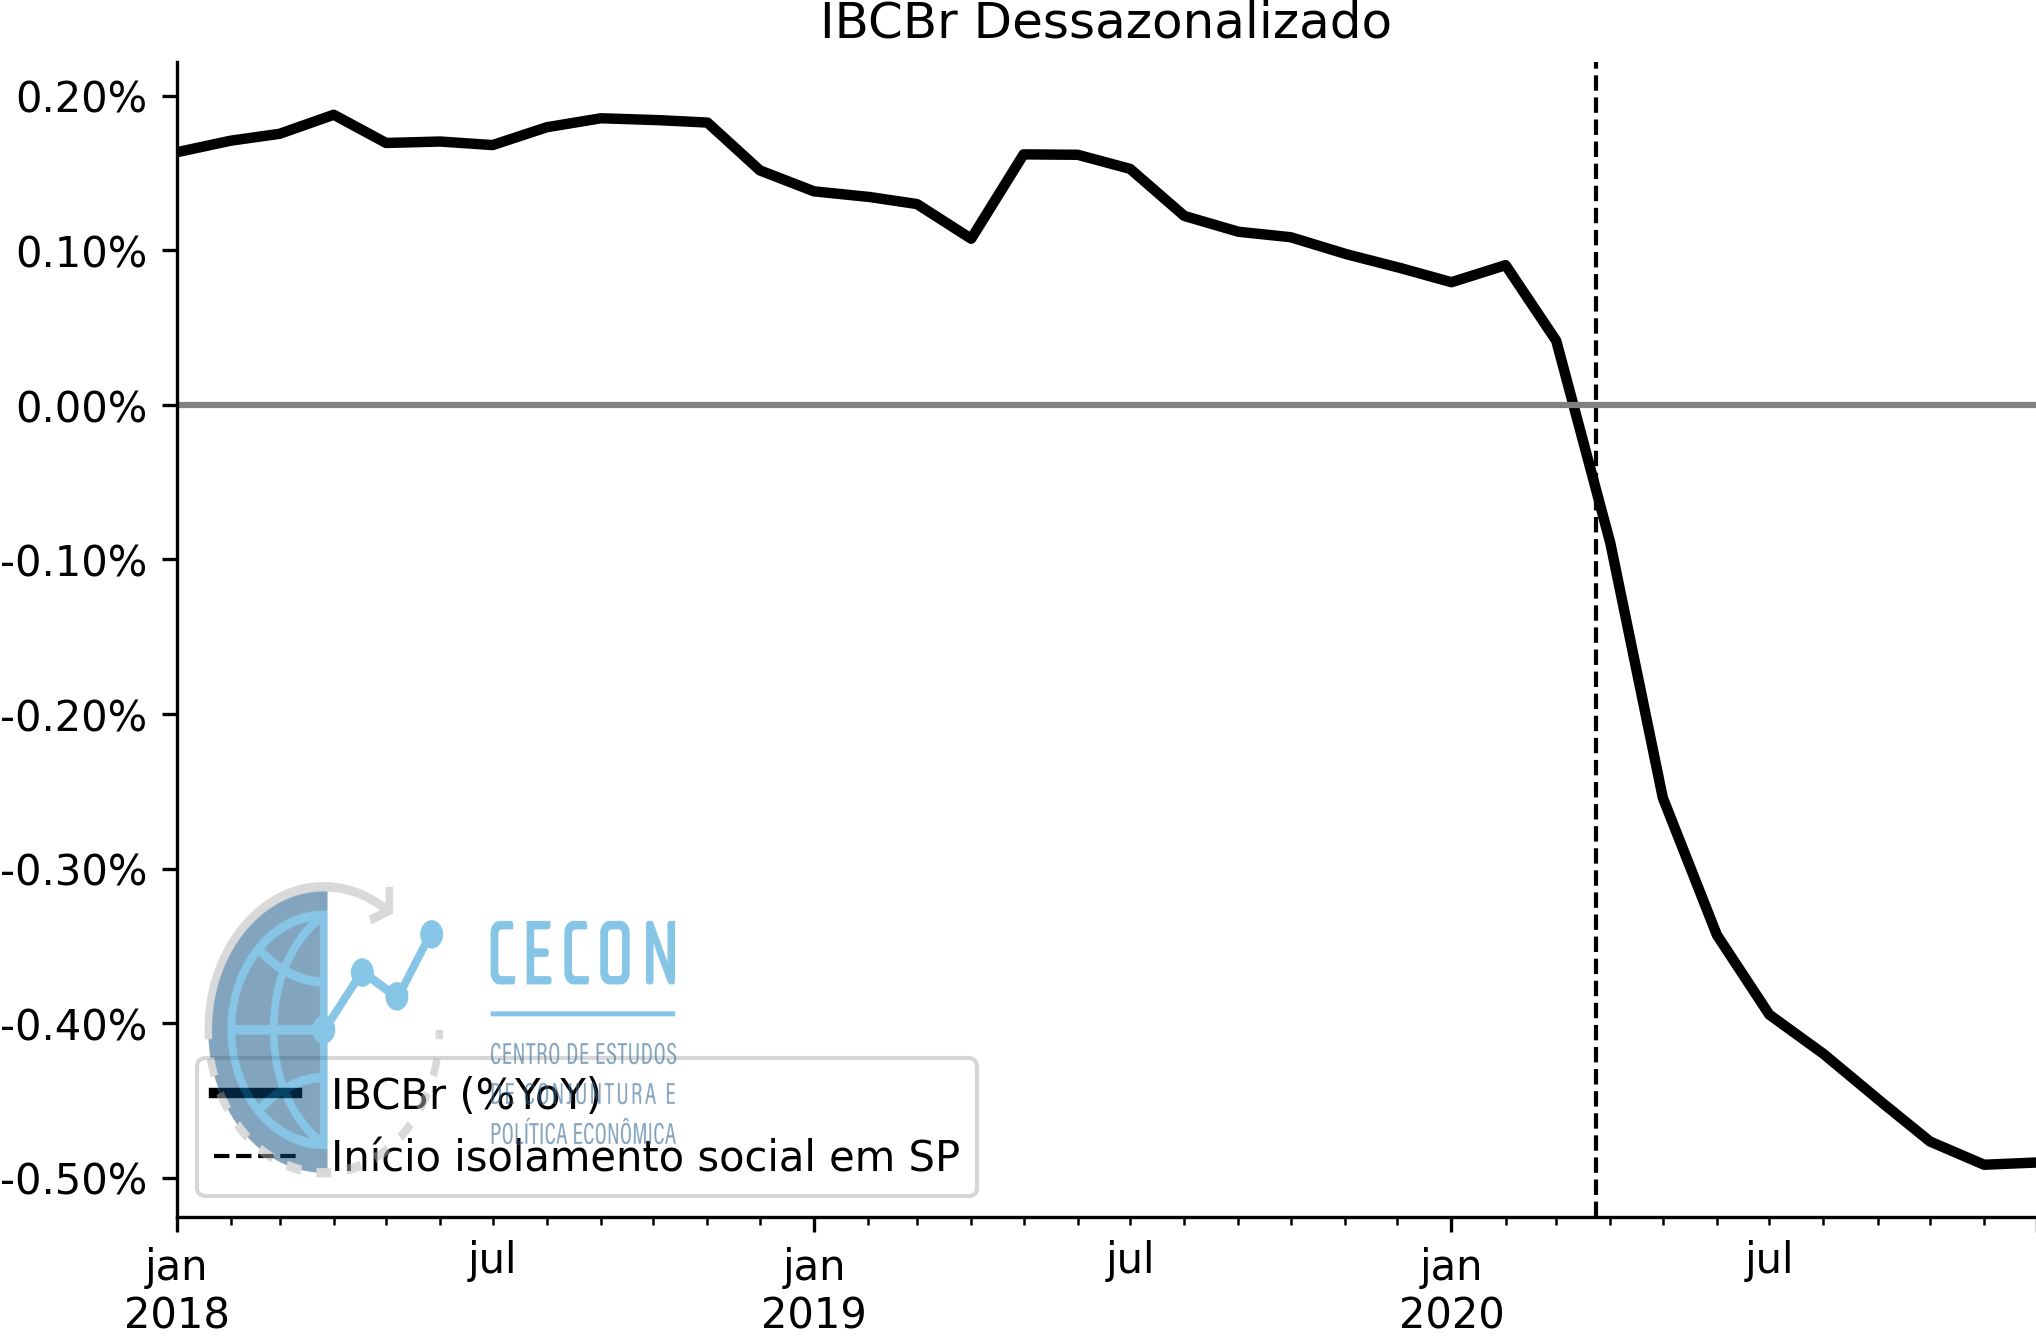
\includegraphics[width=.9\linewidth]{./figs/Antecedente/IBCBr.png}
\end{center}

\subsection*{Tráfego de veículos pesados nas estradas pedagiadas - ABCR - Dados dessazonalizados}
\label{sec:org6151547}


\begin{center}
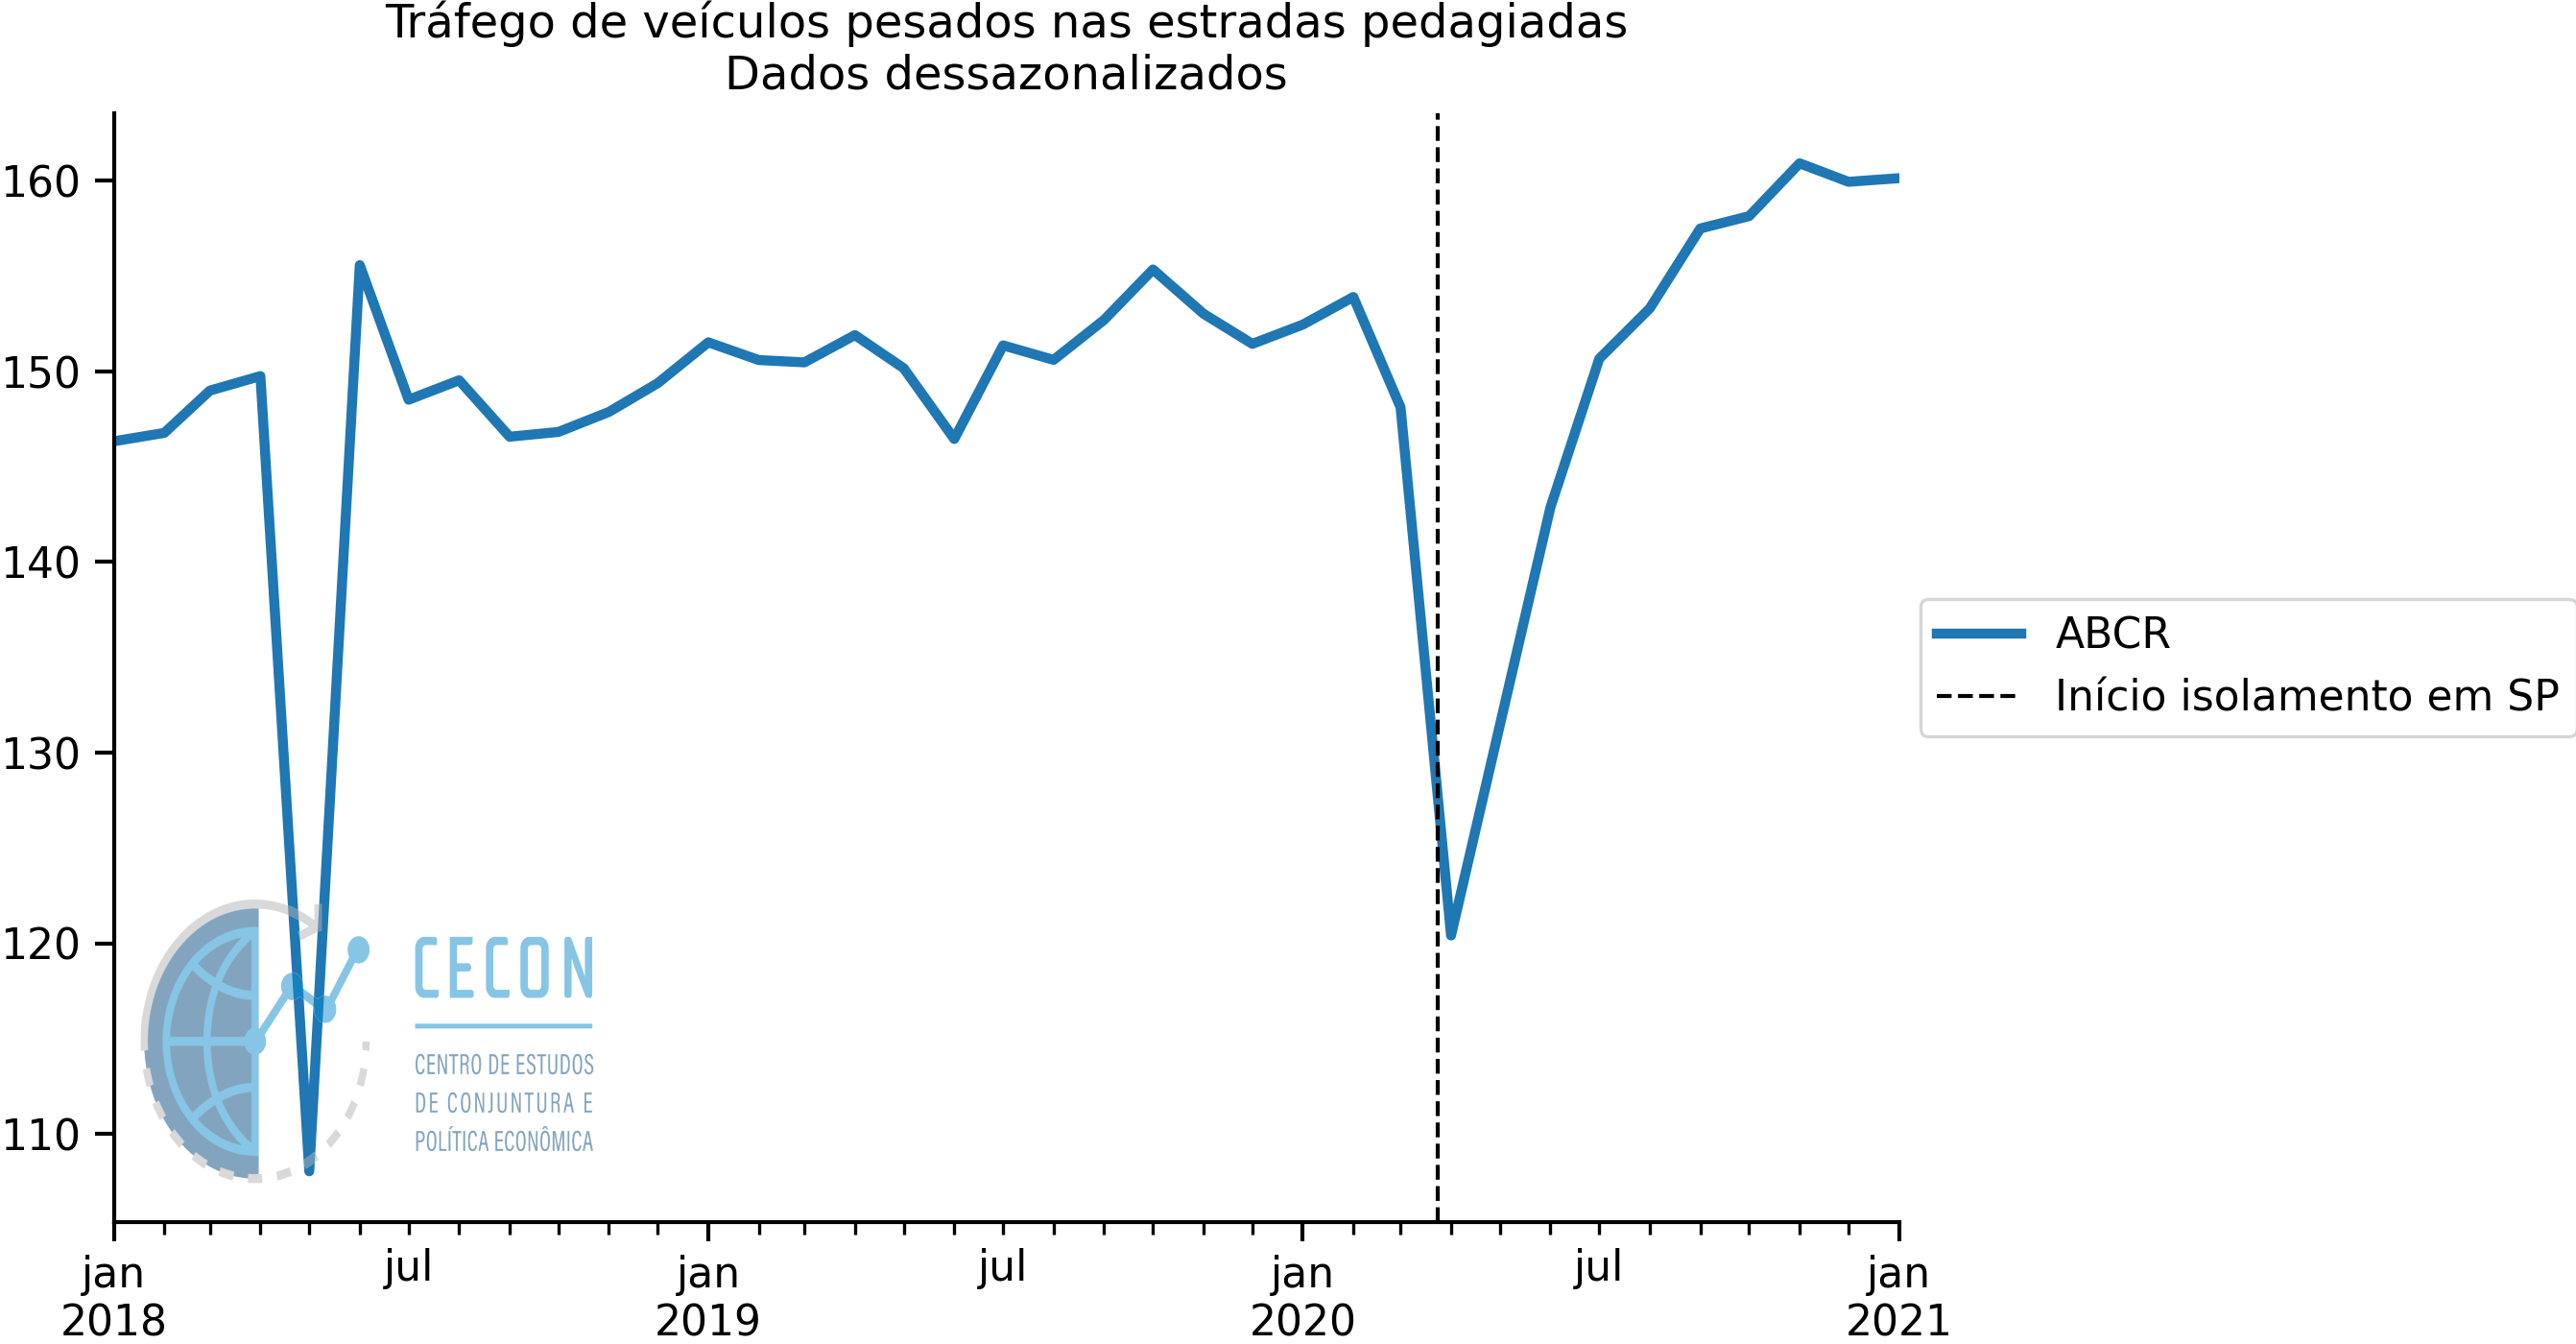
\includegraphics[width=.9\linewidth]{./figs/Setoriais/TrafegoPedagio.png}
\end{center}


\section*{Dados de alta frequência}
\label{sec:org08f3a03}

\subsection*{Bloomberg adaptado ao COVID-19 (\href{https://www.bloomberg.com/news/articles/2020-11-13/alternative-data-show-activity-crashes-as-virus-resurges-chart}{Link})}
\label{sec:orgf037567}

\subsection*{Google Reports: Brasil}
\label{sec:org08c5a62}

\begin{center}
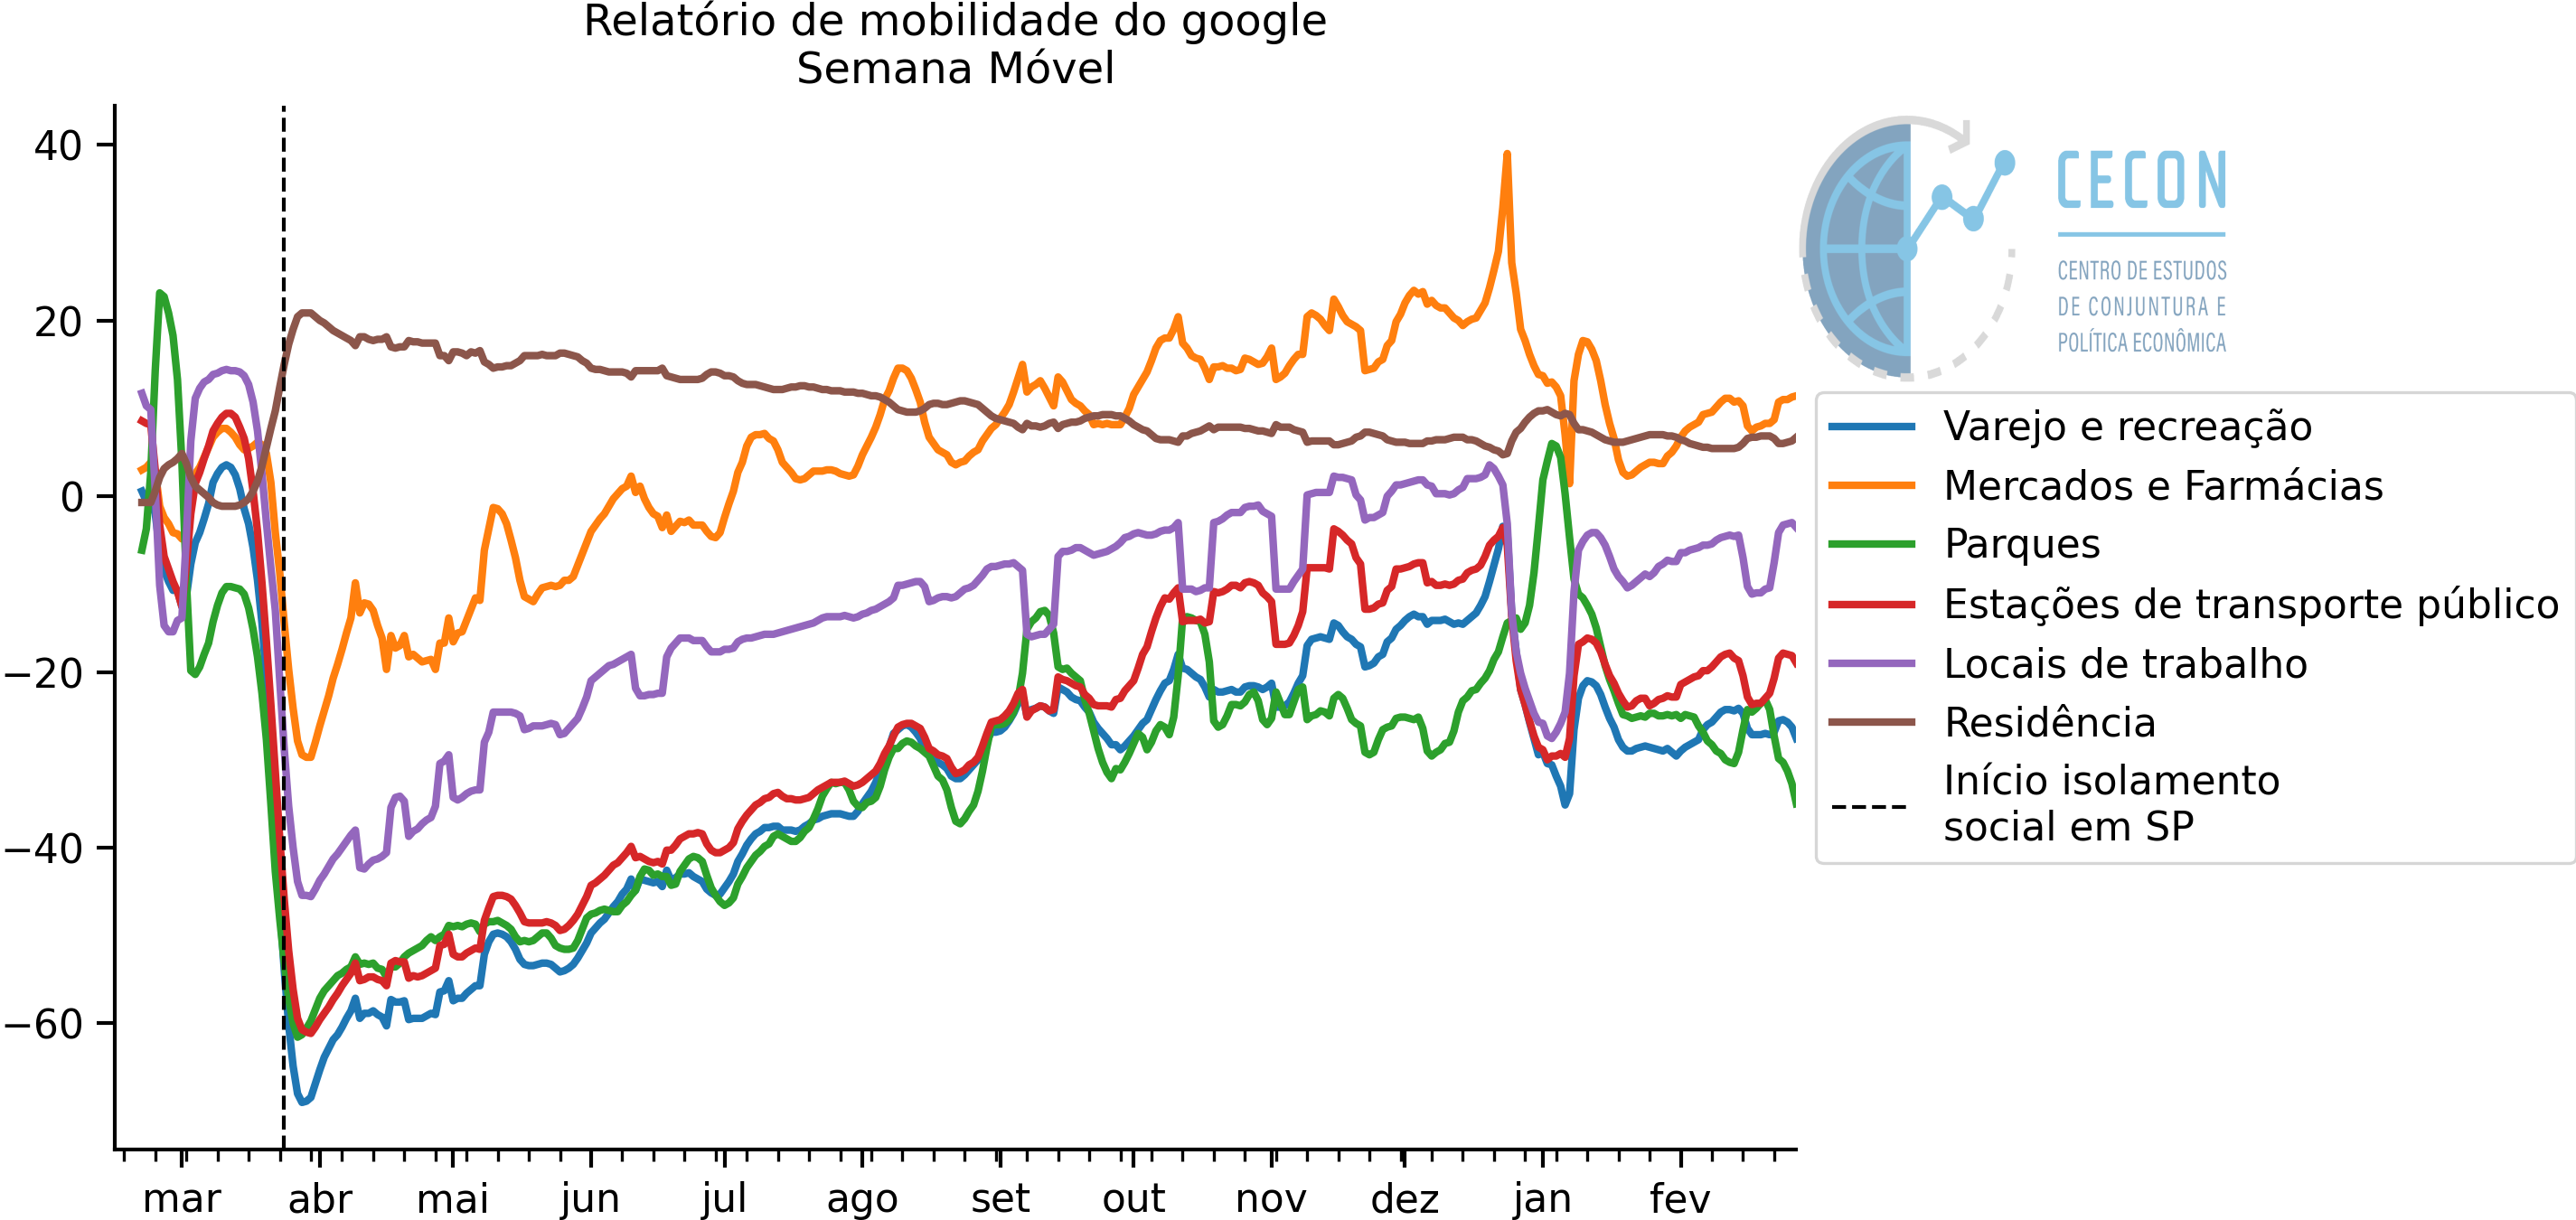
\includegraphics[width=.9\linewidth]{./figs/Granulares/GoogleReport_Brasil.png}
\end{center}

\subsection*{Apple: Tendências de mobilidade}
\label{sec:org7138080}

\begin{center}
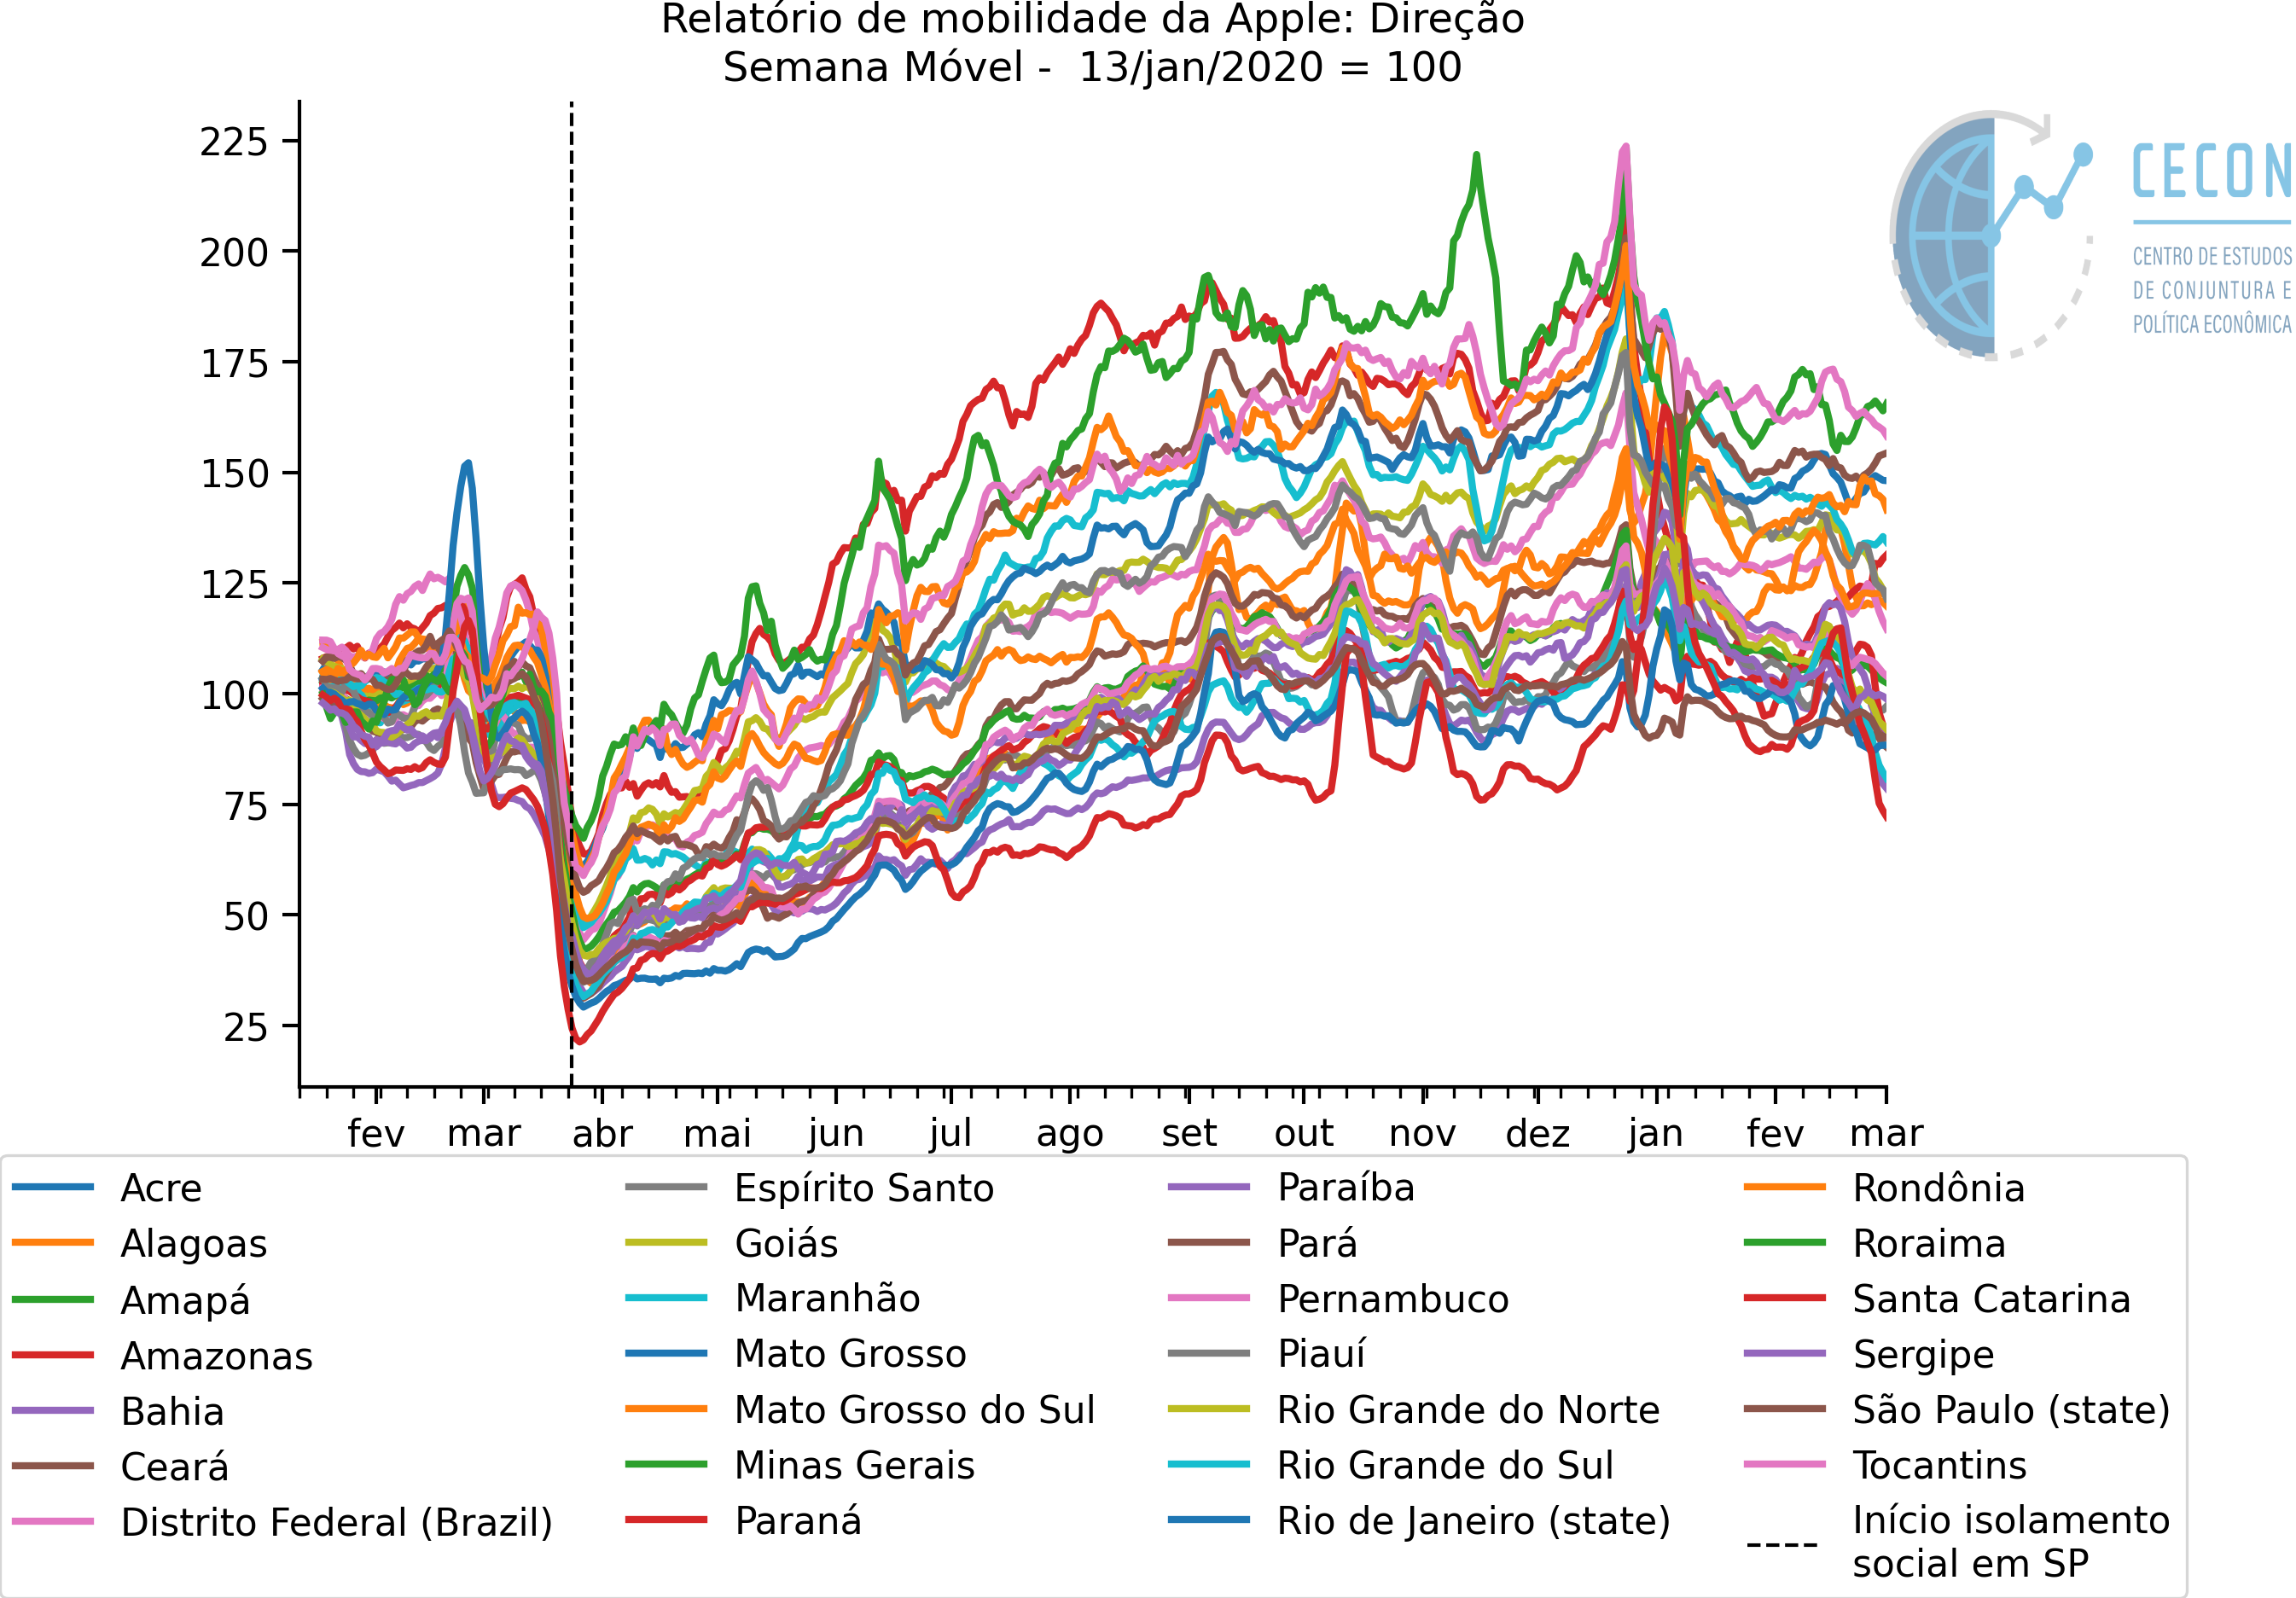
\includegraphics[width=.9\linewidth]{./figs/Granulares/AppleReport_Brasil.png}
\end{center}

\subsection*{Waze: \(\Delta \%\) Km}
\label{sec:org42650bd}

\begin{center}
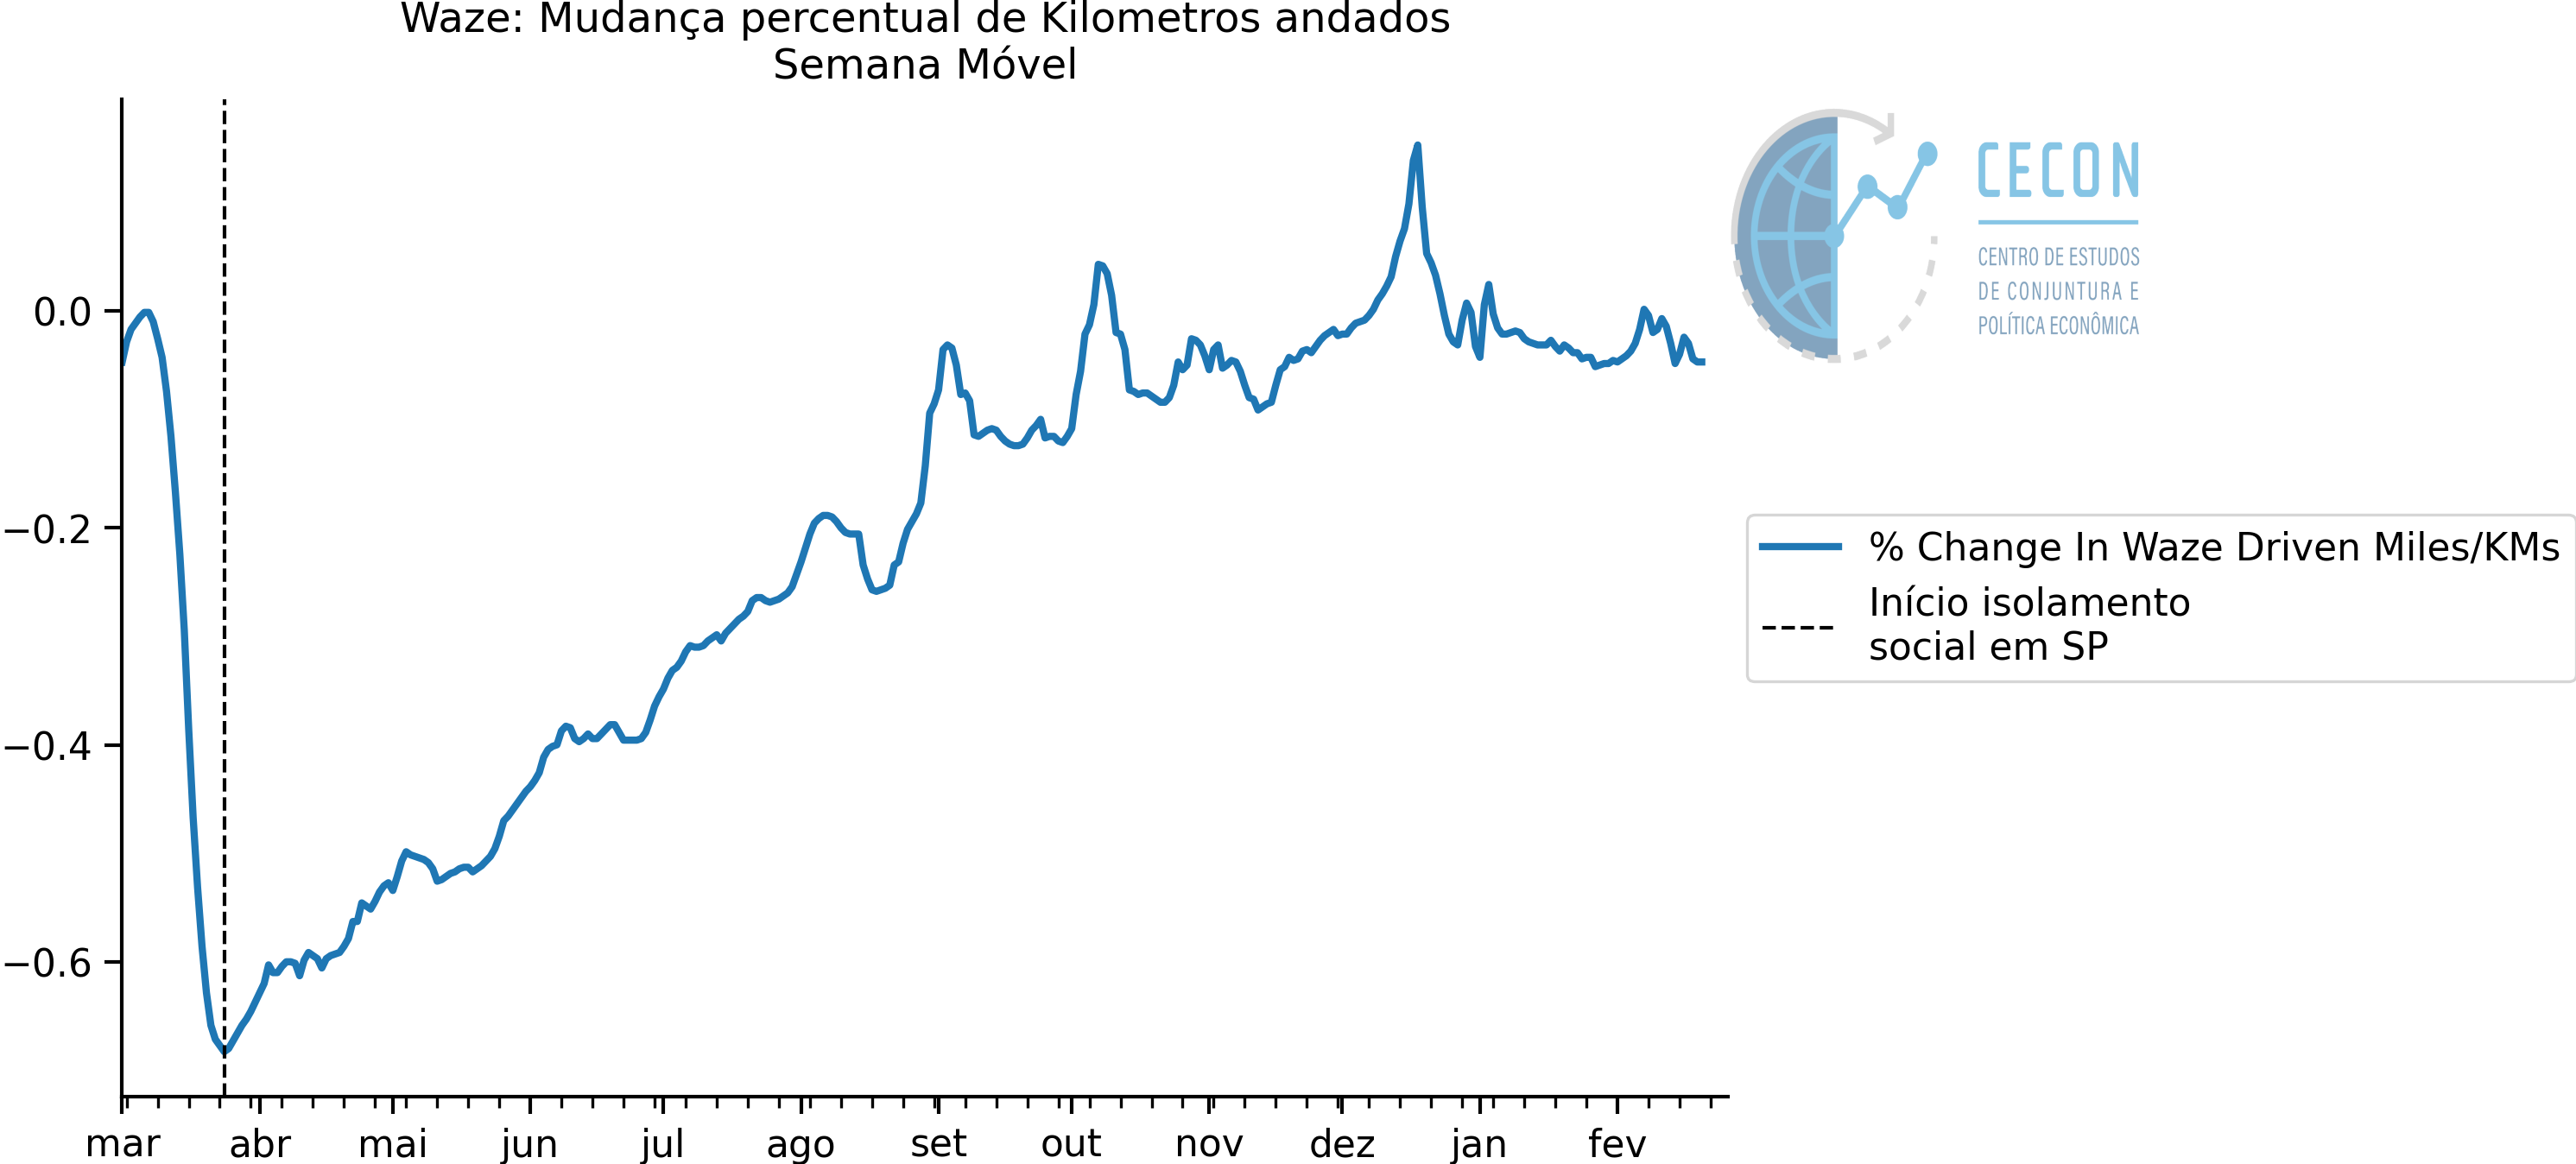
\includegraphics[width=.9\linewidth]{./figs/Granulares/Waze_Brasil.png}
\end{center}

\subsection*{TomTom: Congestionamento}
\label{sec:orgb3f2bd5}

\begin{center}
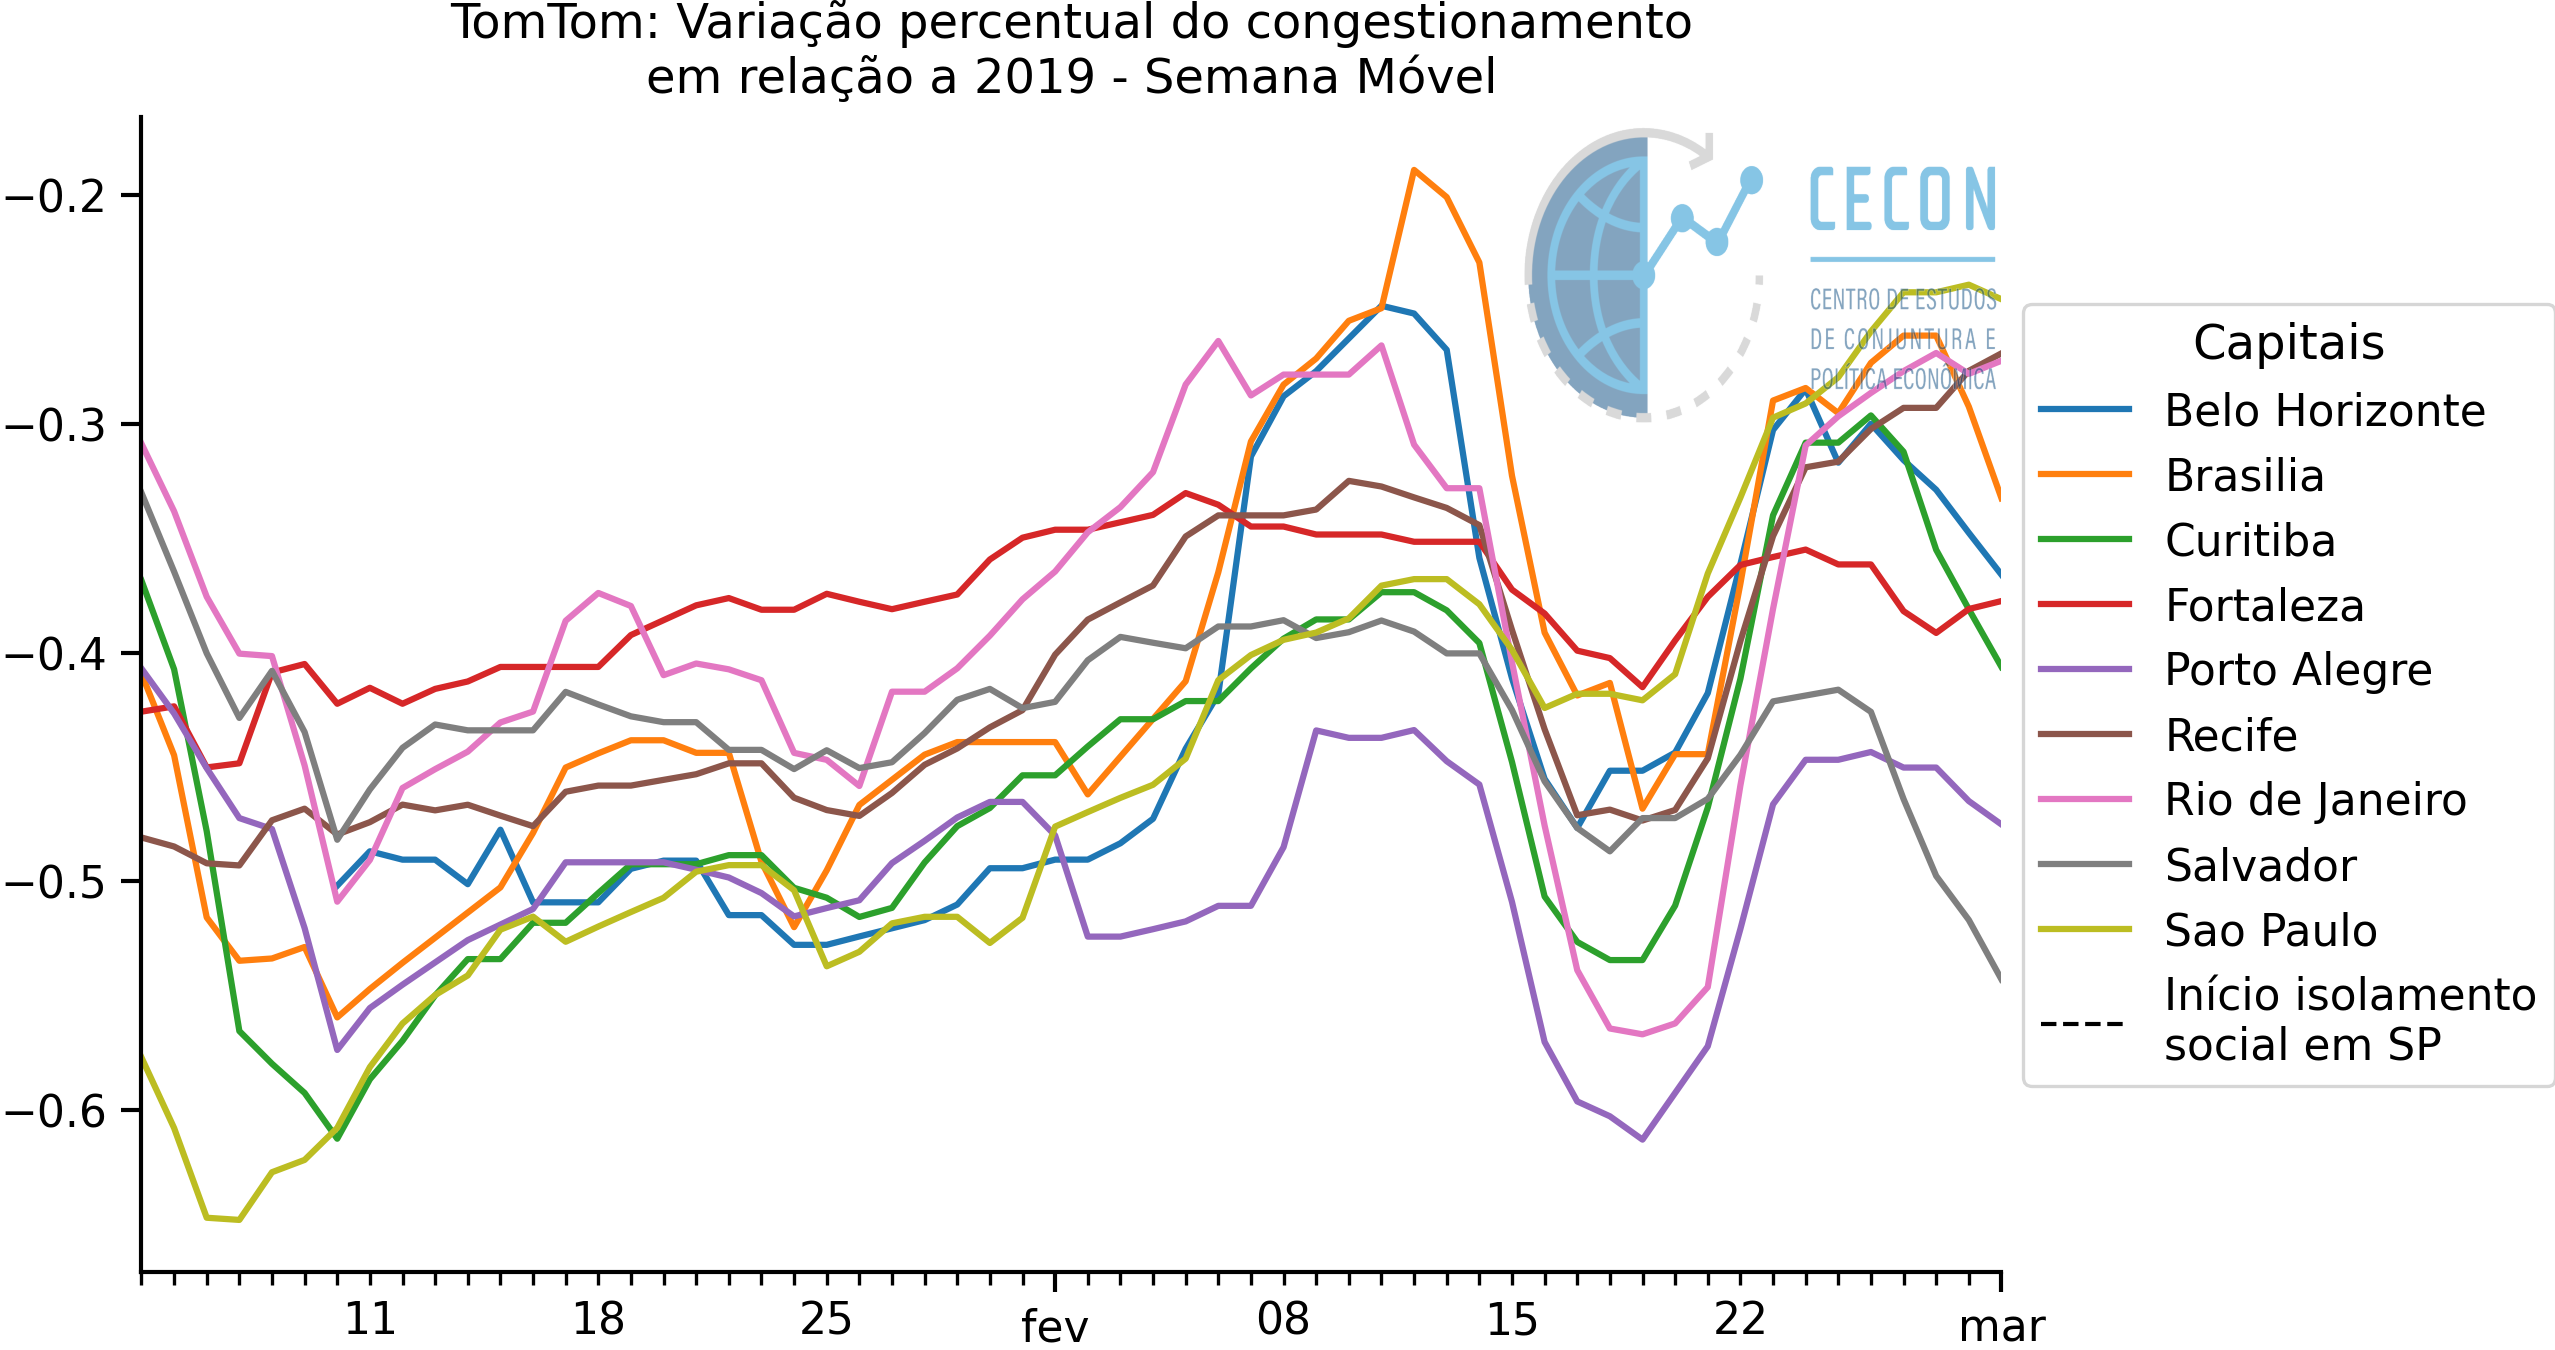
\includegraphics[width=.9\linewidth]{./figs/Granulares/TomTom_Brasil.png}
\end{center}

\section*{Atividade}
\label{sec:org086af36}



\subsection*{Trimestre Contra trimestre imediatamente anterior}
\label{sec:orgdb4d554}

\begin{center}
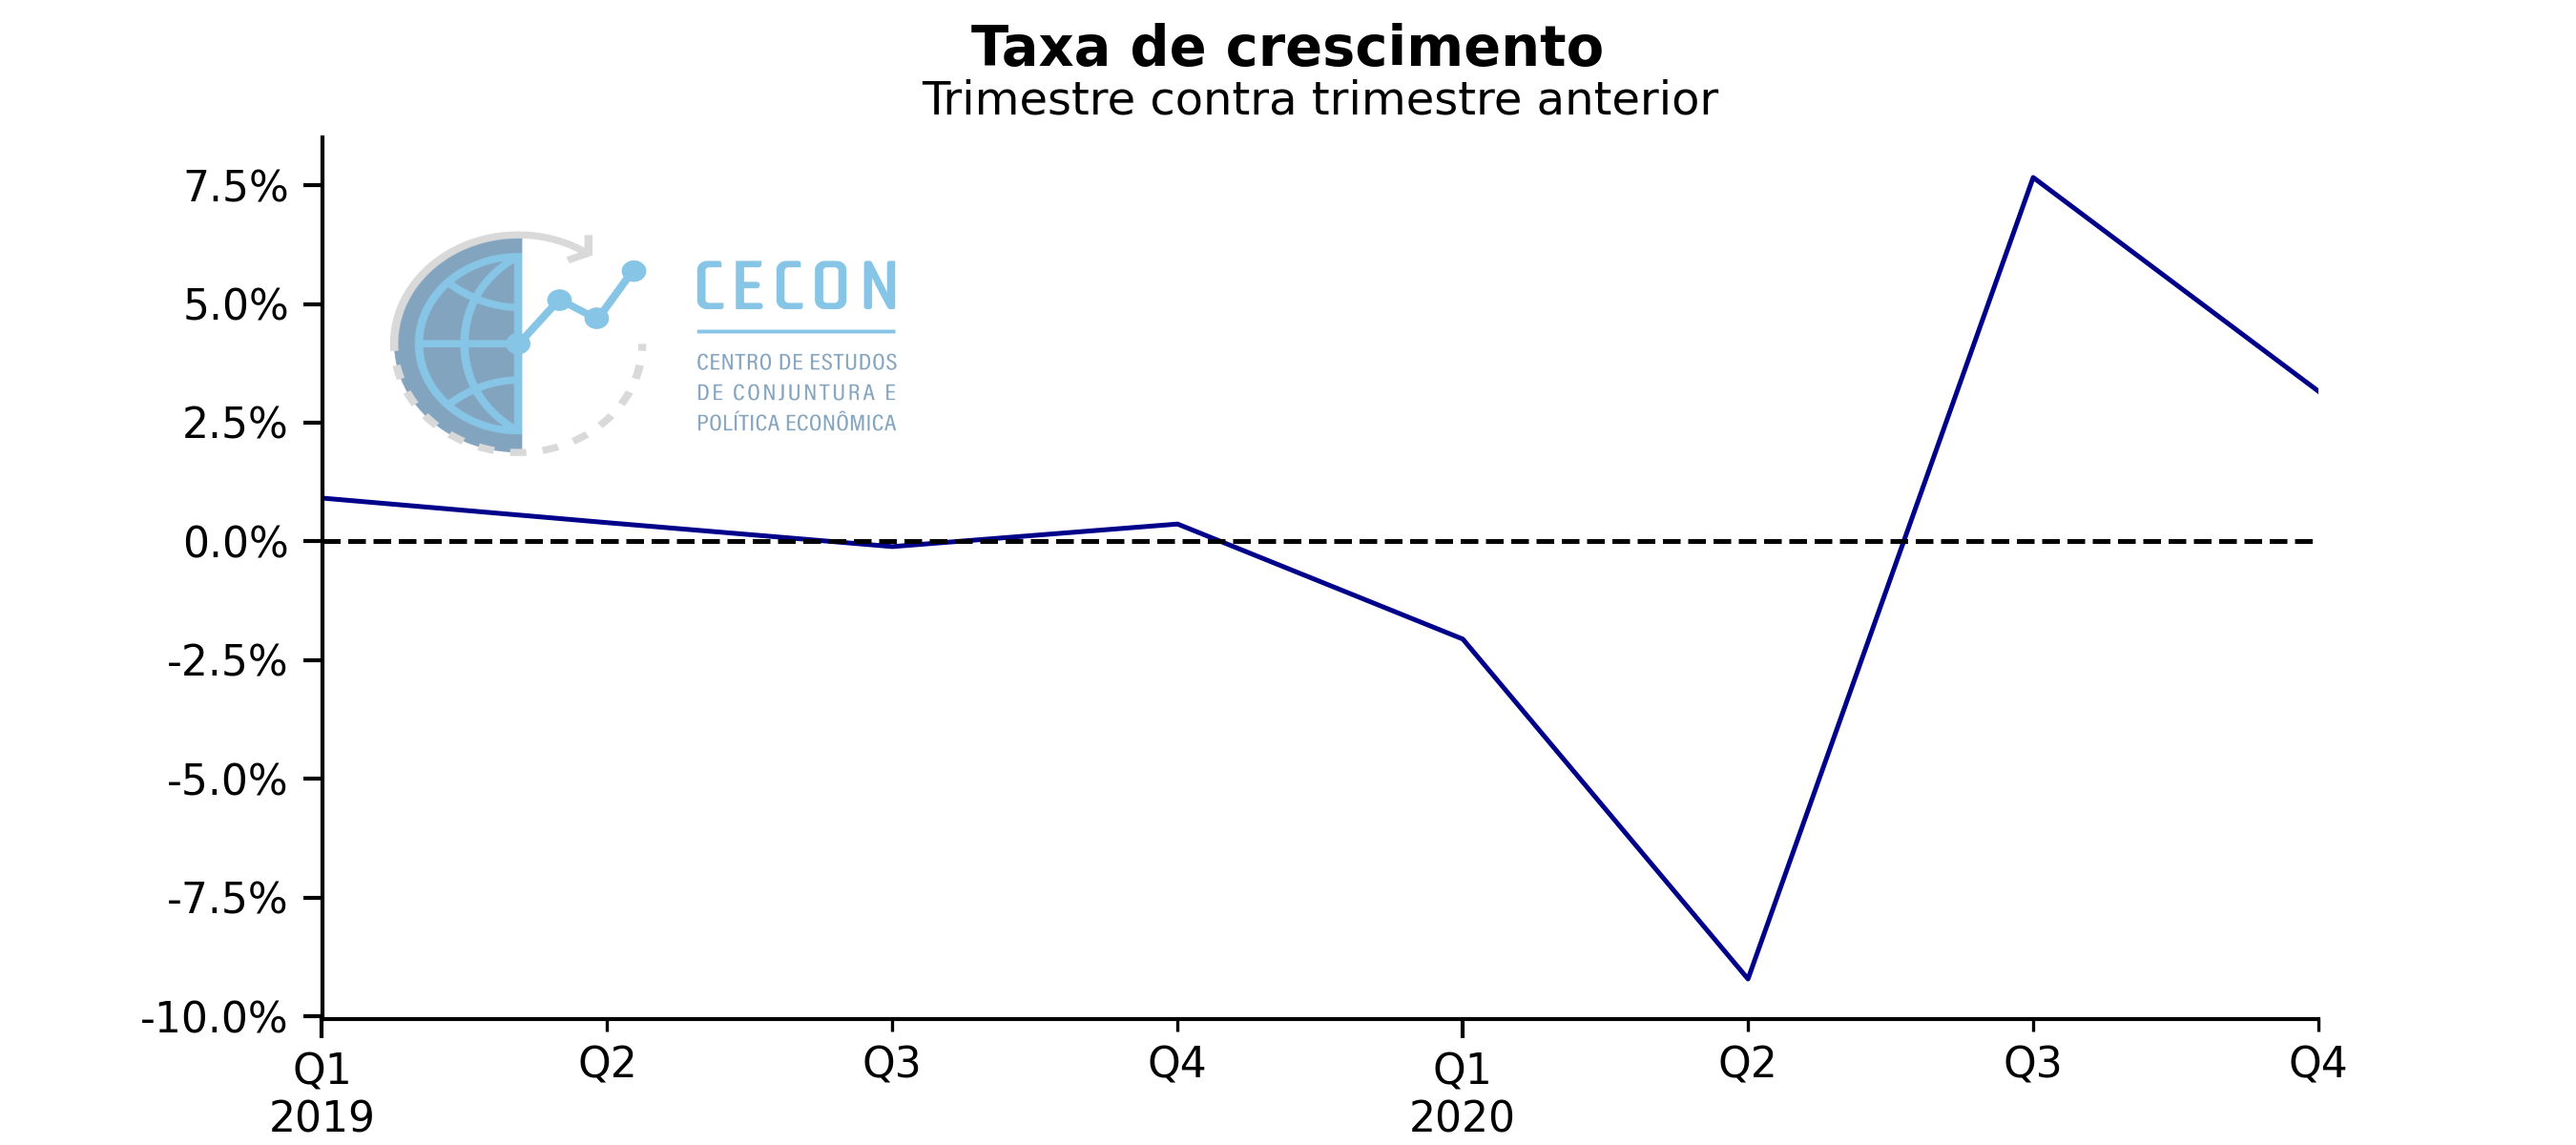
\includegraphics[width=.9\linewidth]{./figs/PIB/PIB.png}
\end{center}

\subsection*{Trimestre Contra mesmo trimestre do ano anterior}
\label{sec:orgc4a835b}

\begin{center}
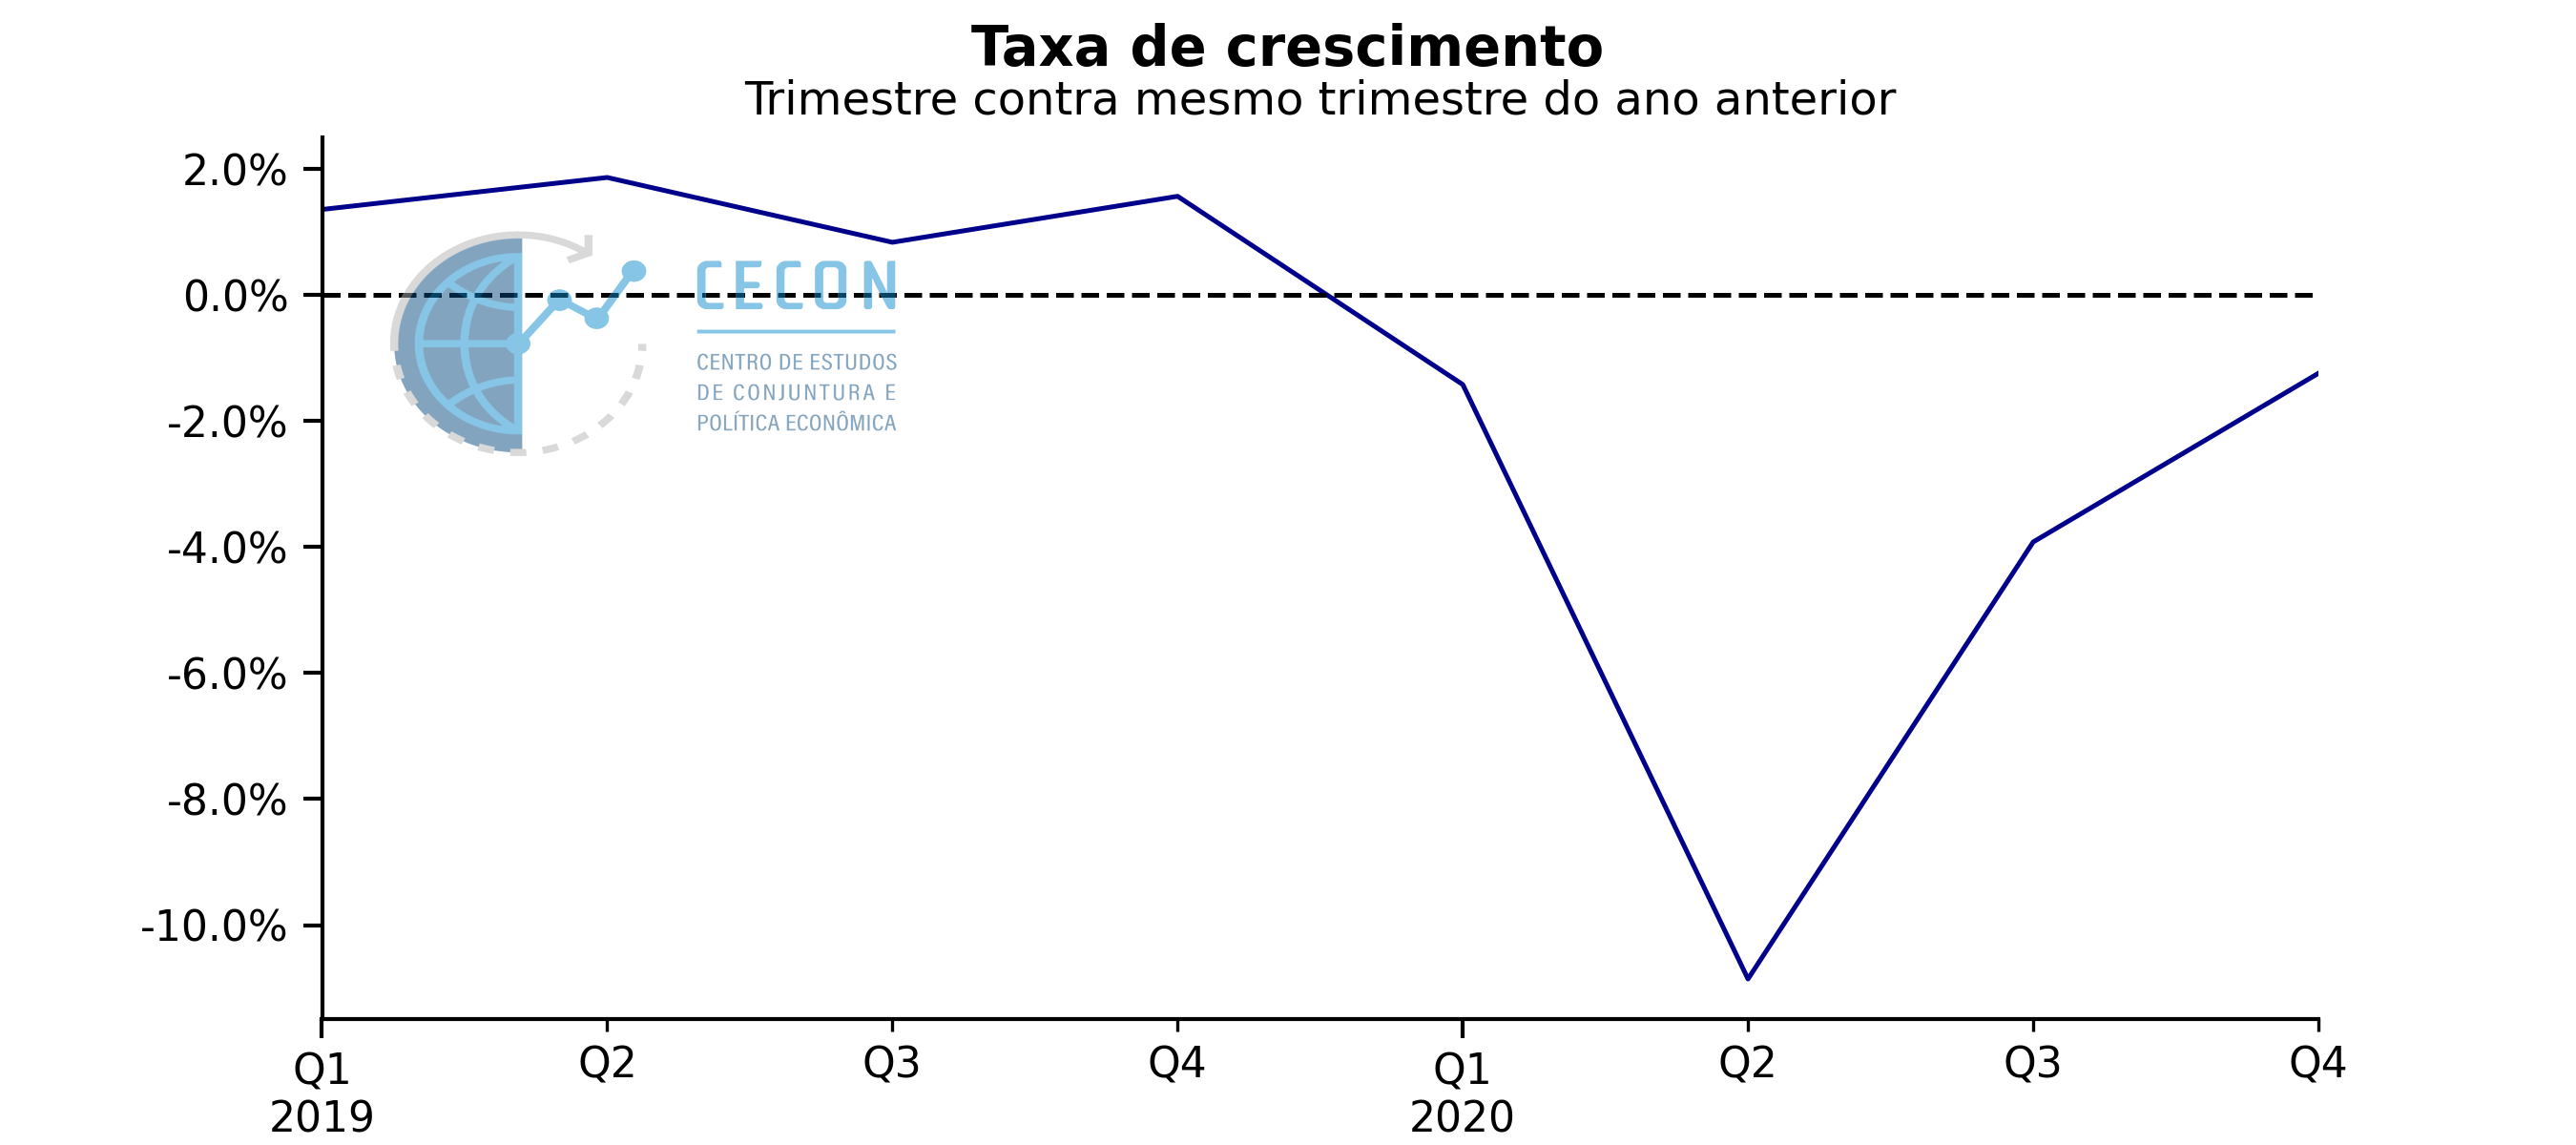
\includegraphics[width=.9\linewidth]{./figs/PIB/PIB_YoY.png}
\end{center}

\subsection*{Agropecuária}
\label{sec:org4bb26c1}

\begin{center}
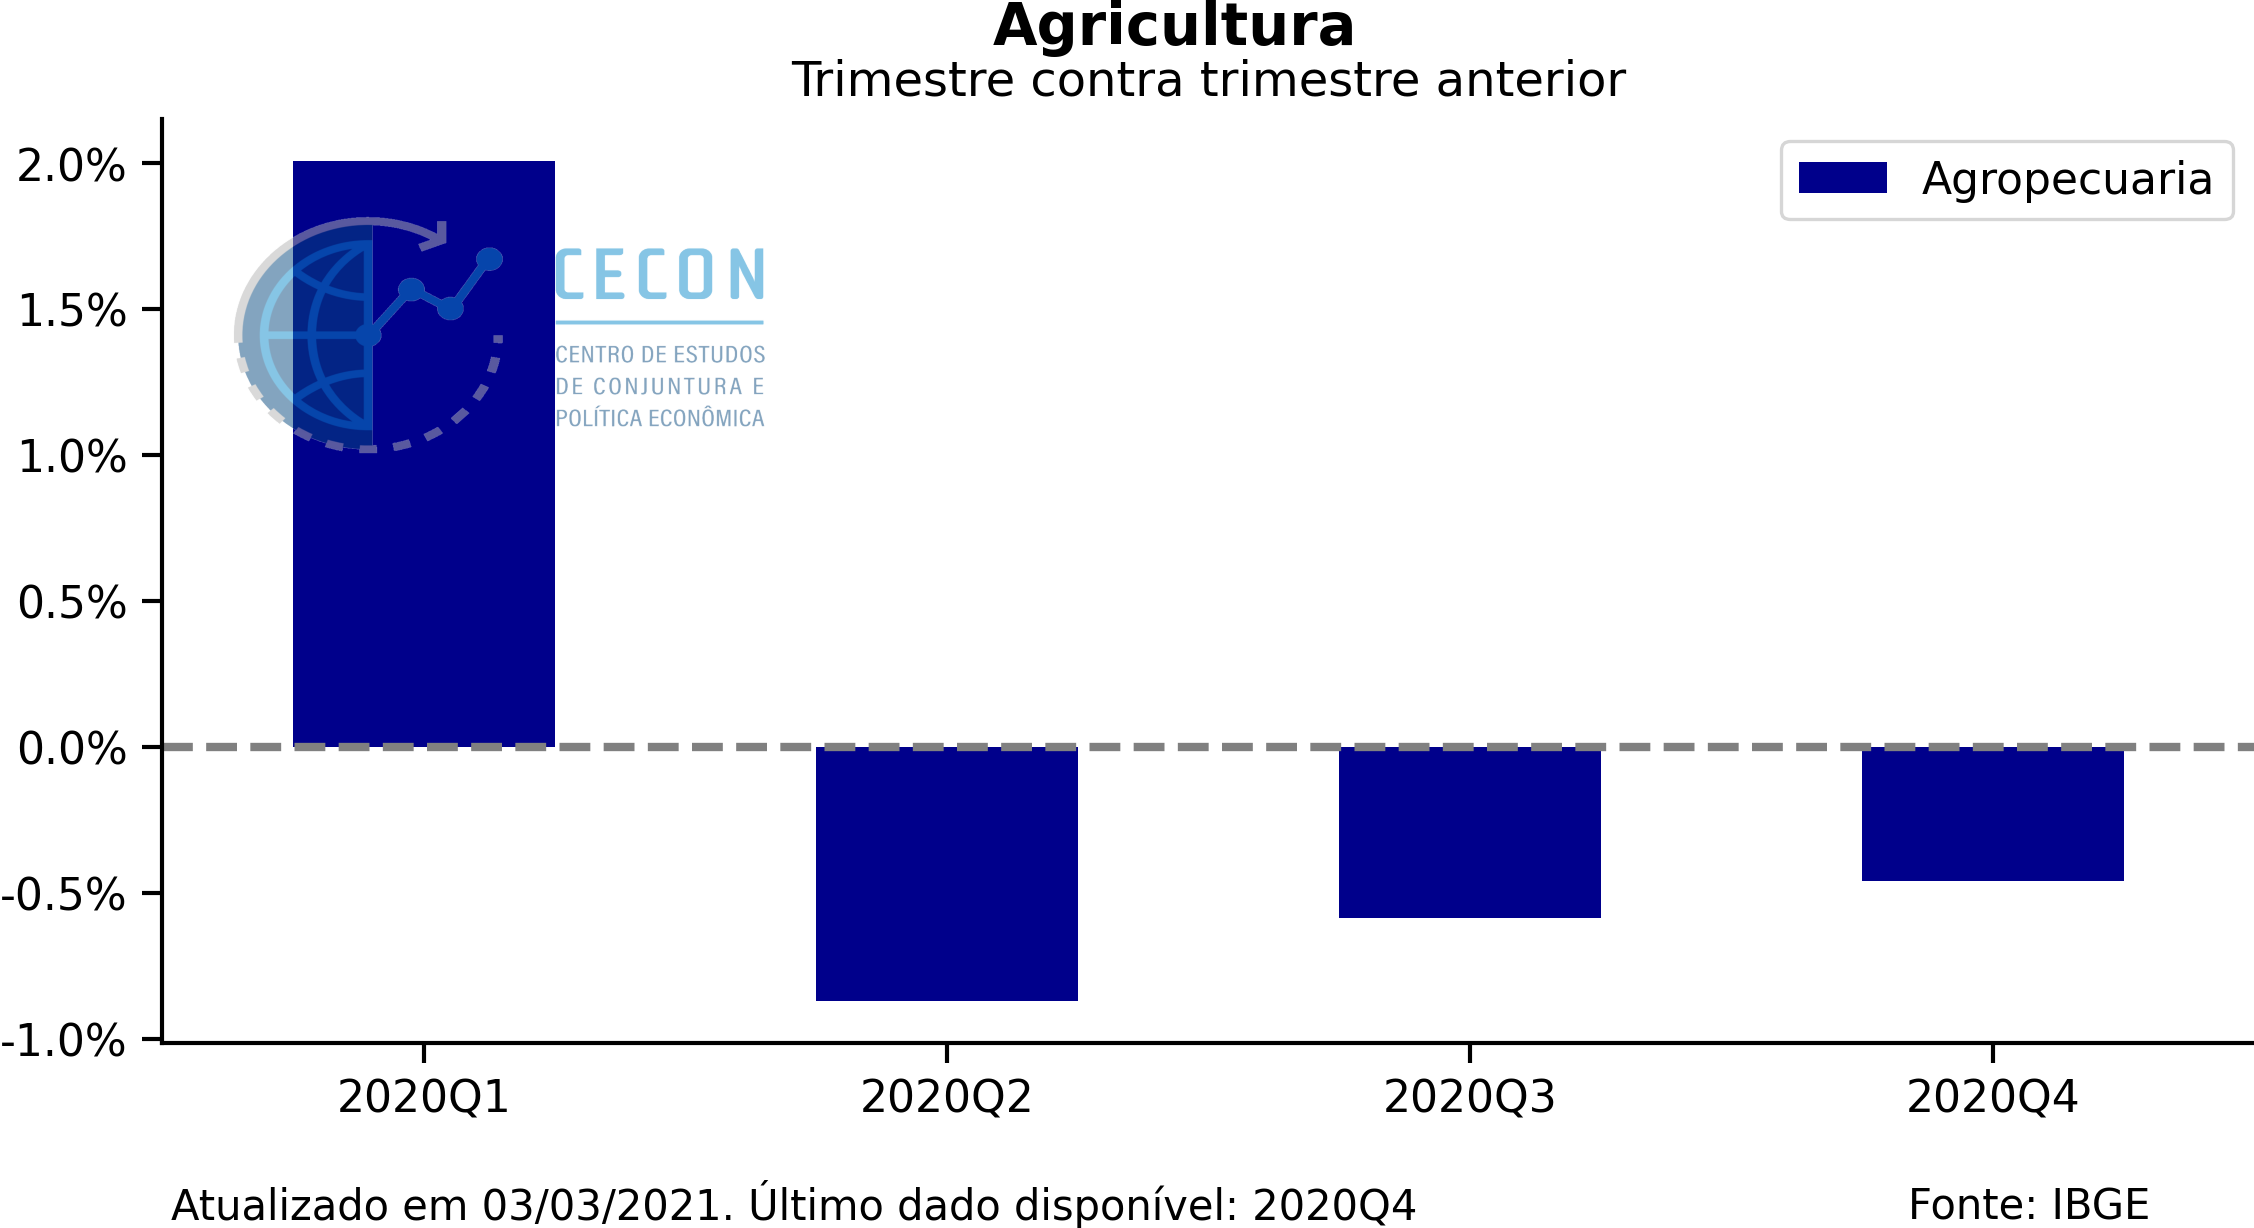
\includegraphics[width=.9\linewidth]{./figs/PIB/Agropecuaria.png}
\end{center}

\subsection*{Indústria}
\label{sec:orgaafde92}

\begin{center}
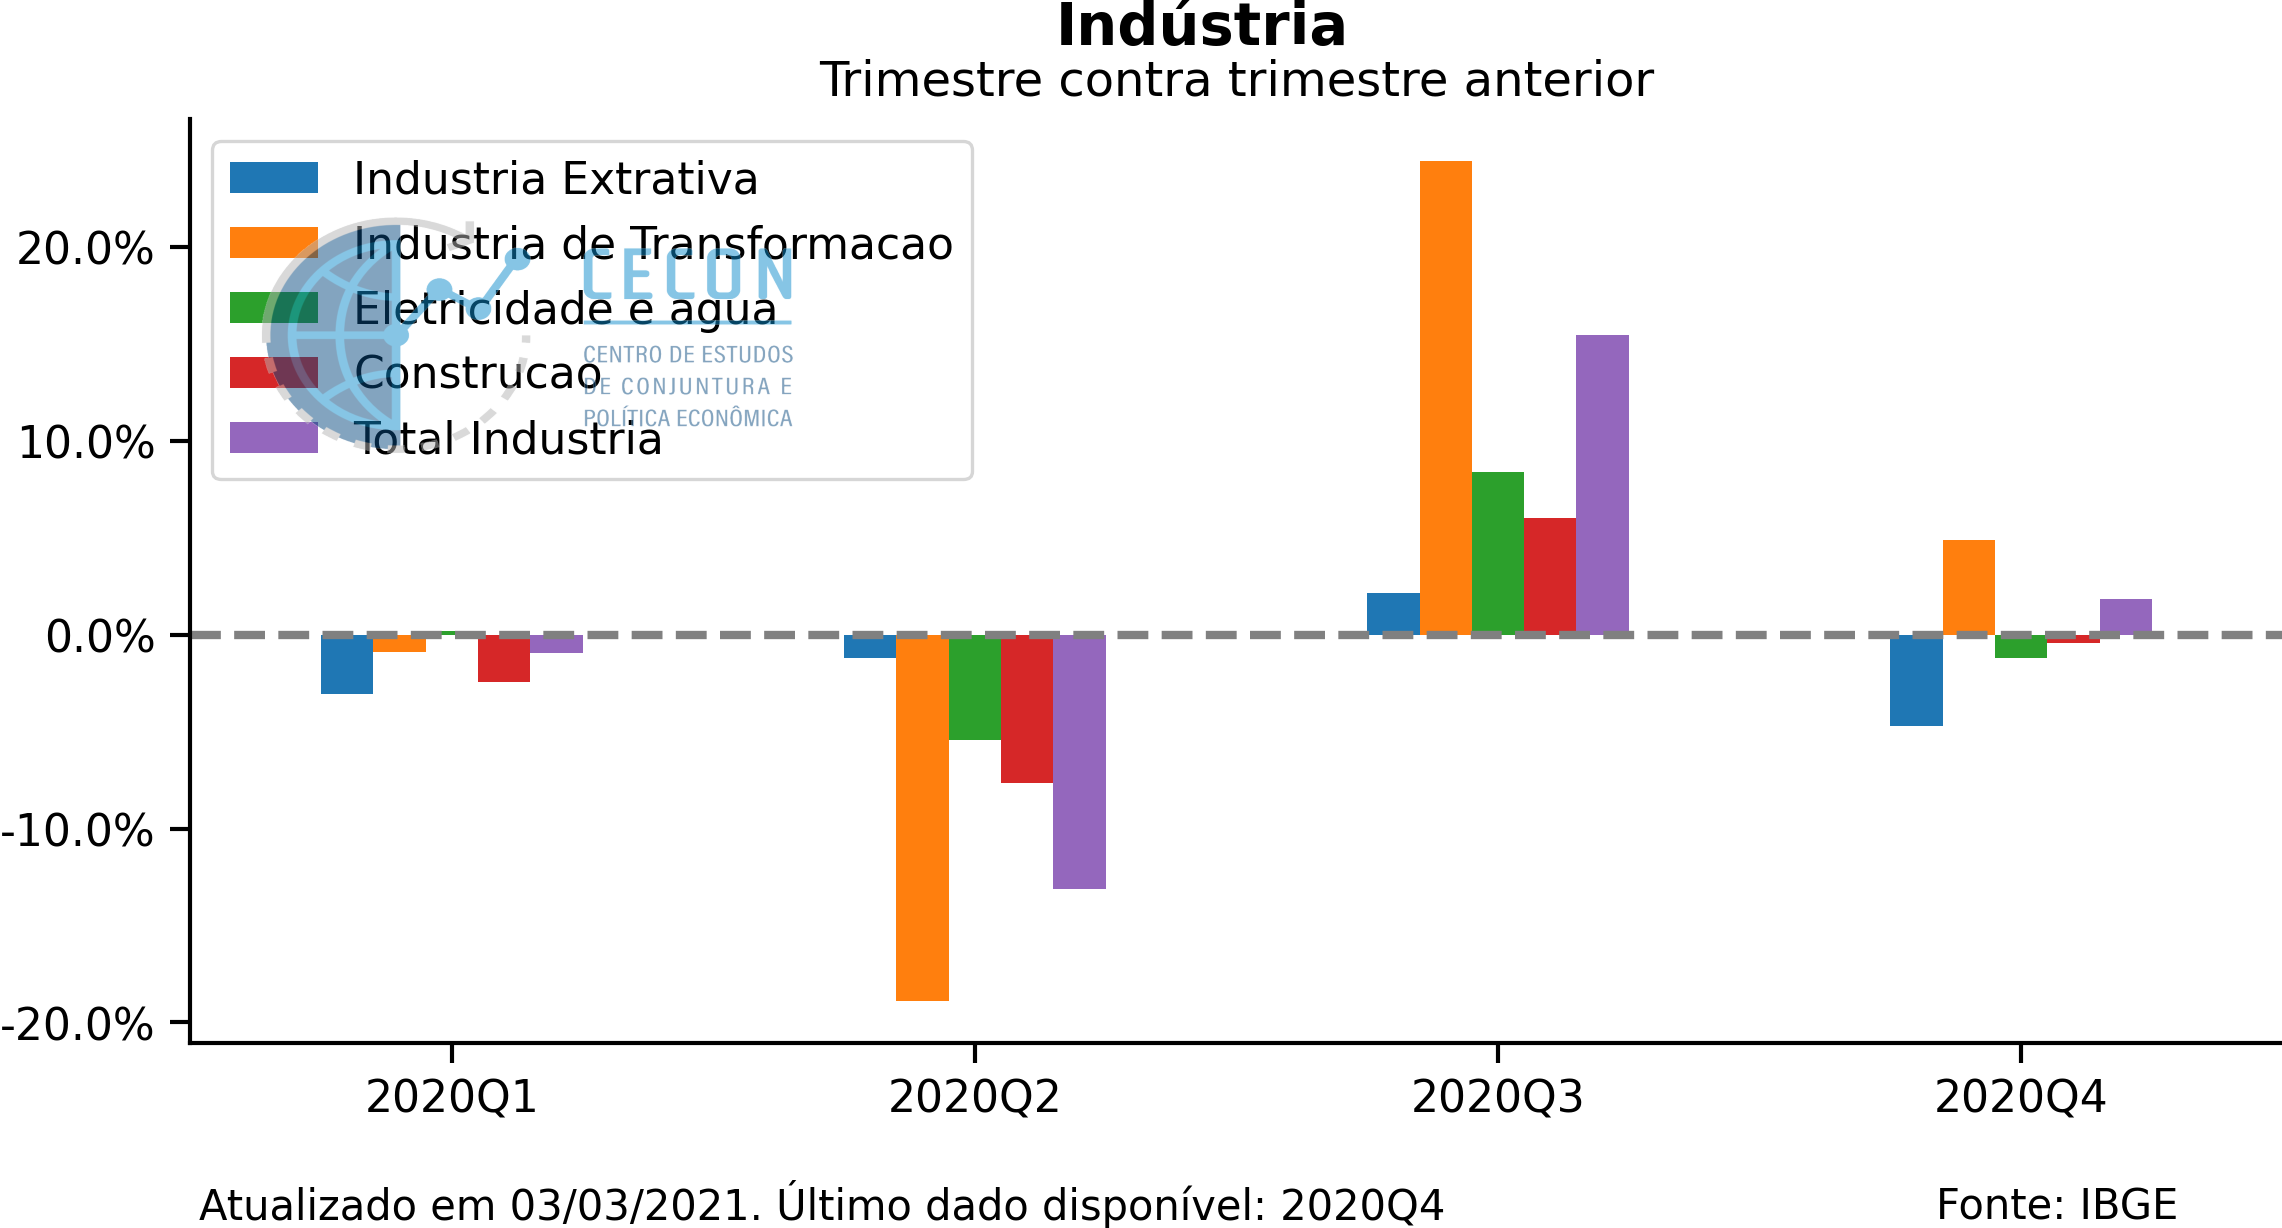
\includegraphics[width=.9\linewidth]{./figs/PIB/Industria.png}
\end{center}


\subsection*{Serviços}
\label{sec:org16dcd26}

\begin{center}
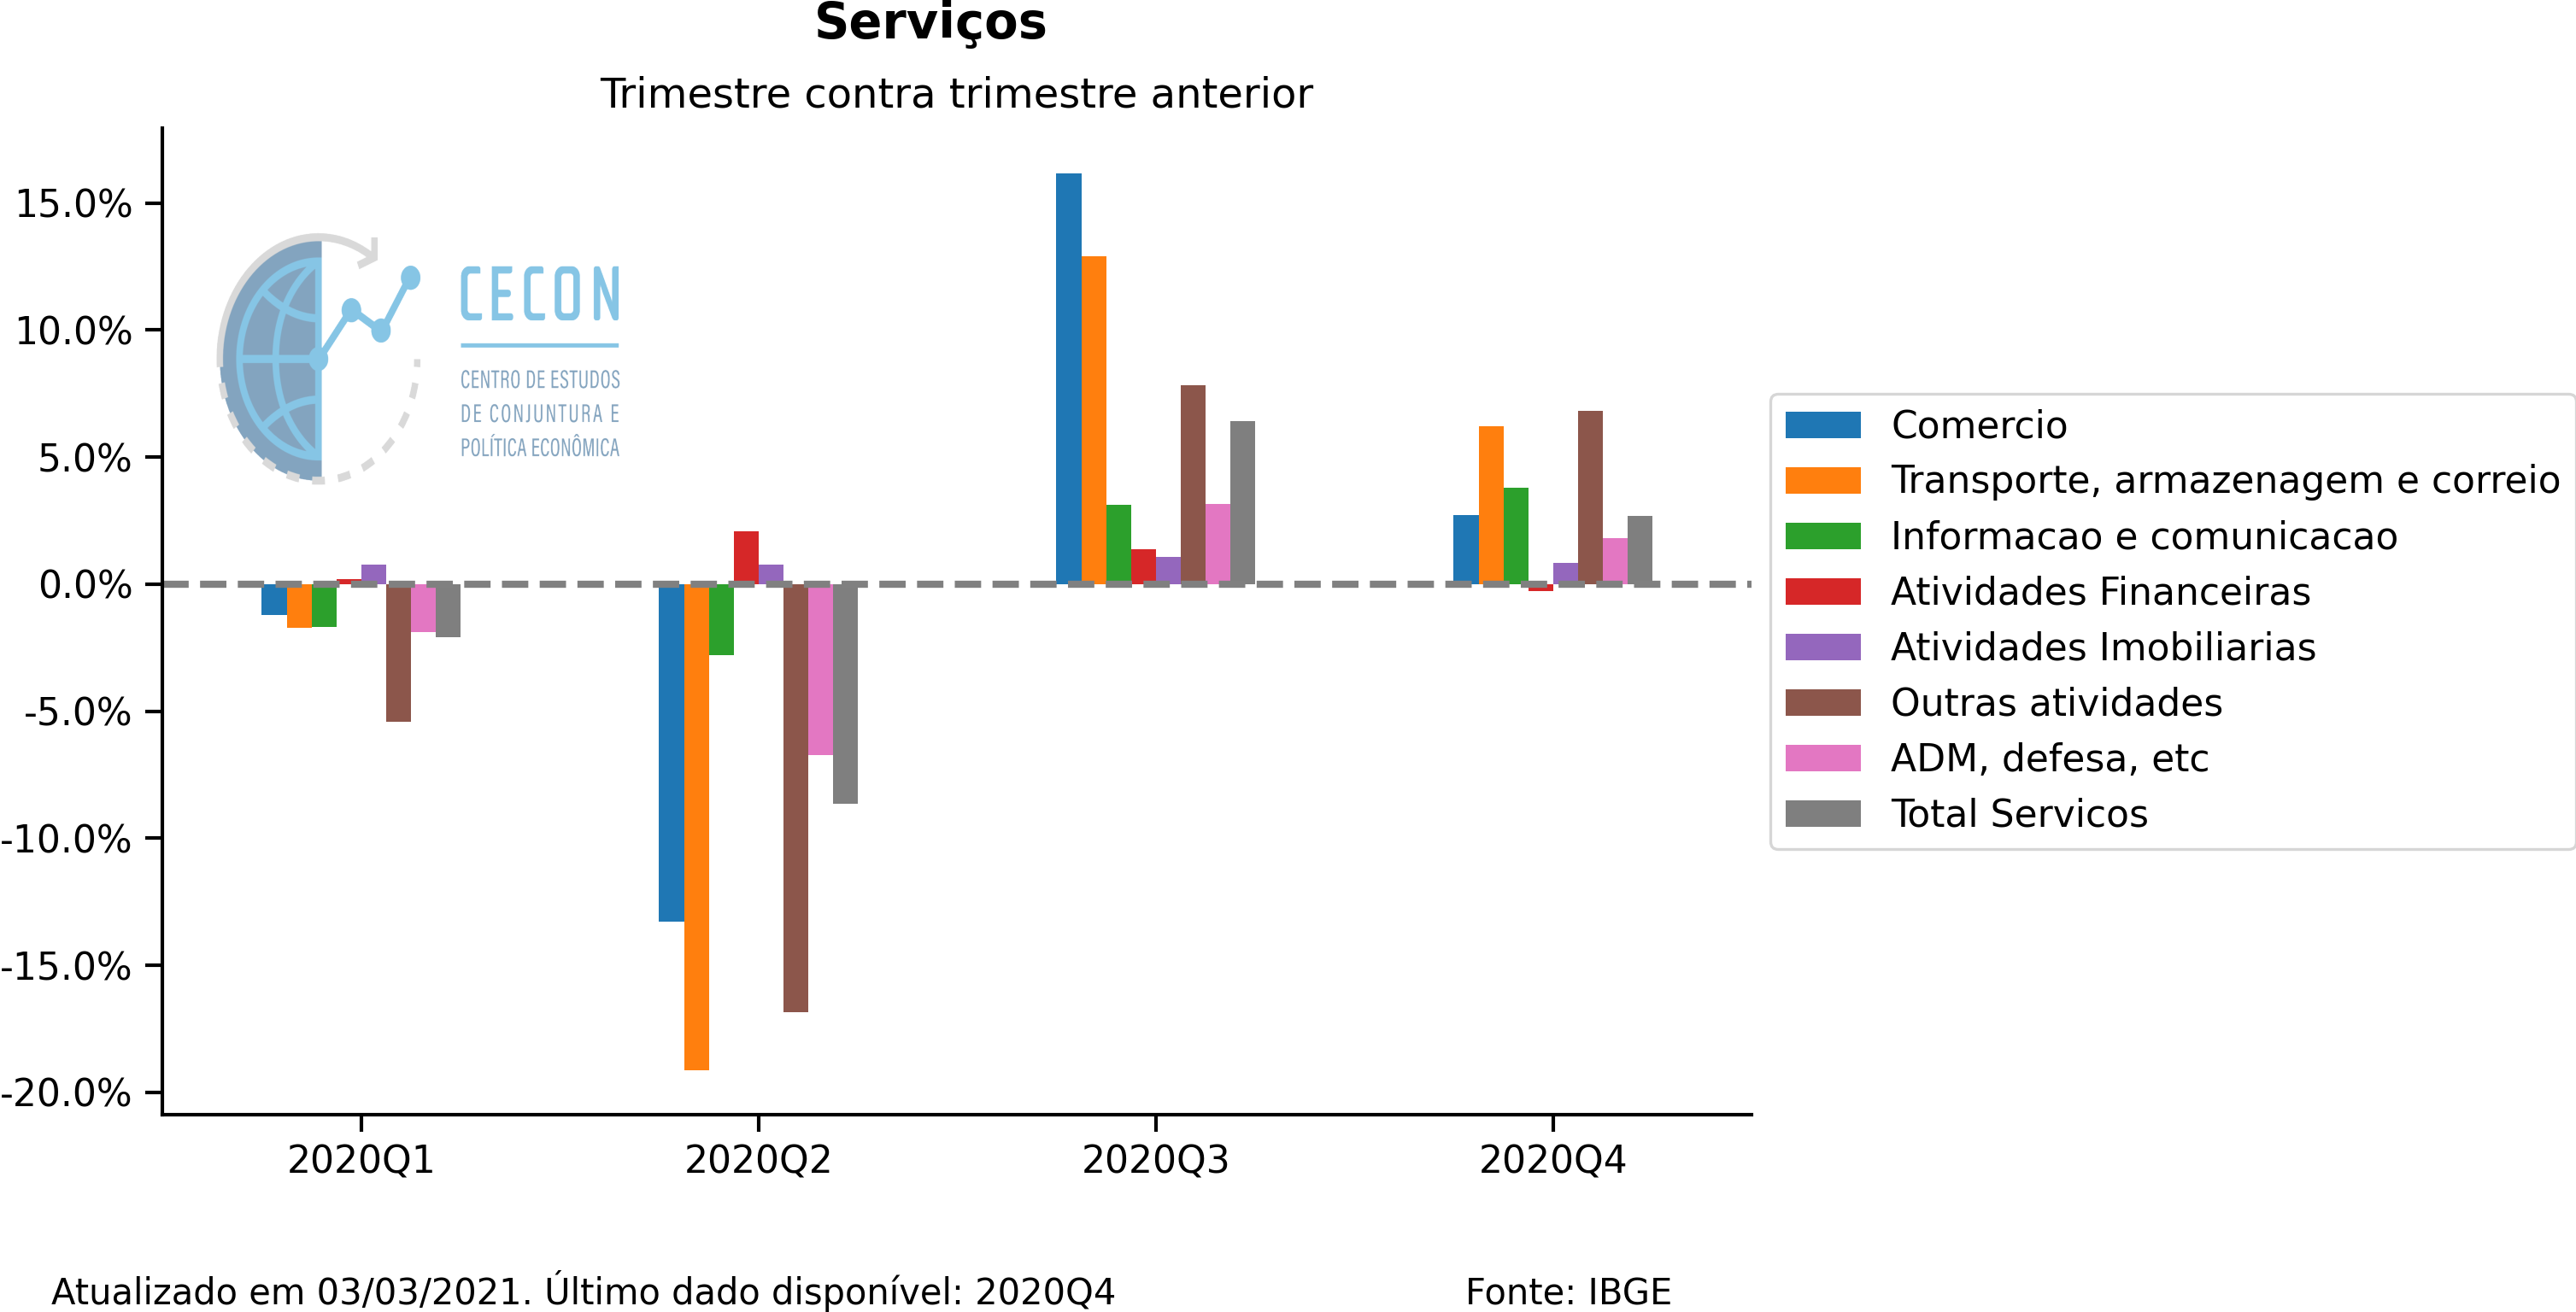
\includegraphics[width=.9\linewidth]{./figs/PIB/Servicos.png}
\end{center}

\subsection*{Demanda}
\label{sec:org0be2aef}

\begin{center}
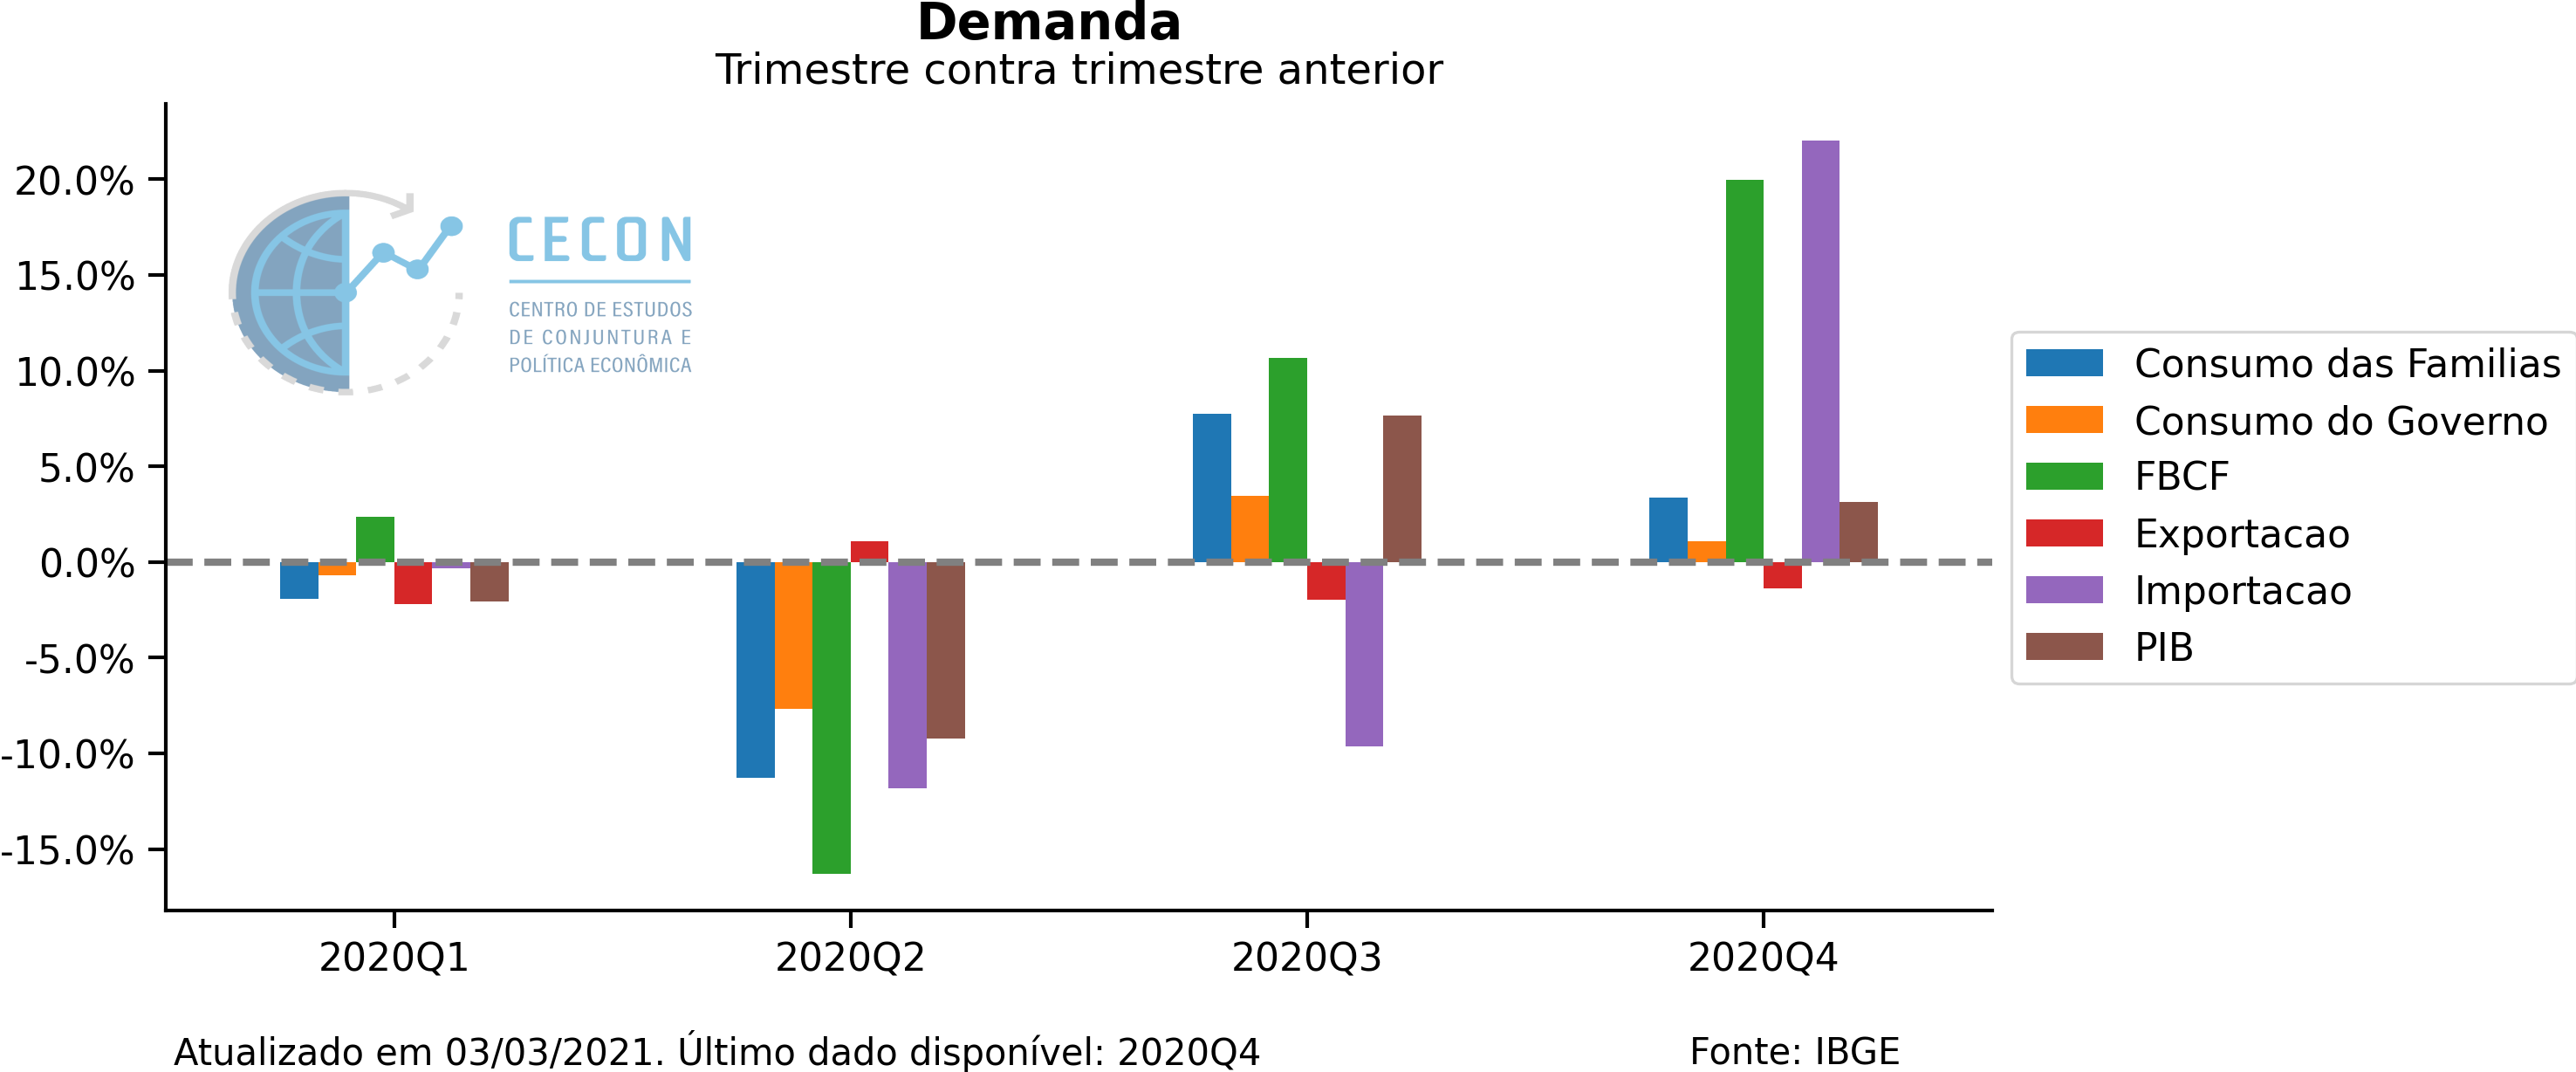
\includegraphics[width=.9\linewidth]{./figs/PIB/Demanda.png}
\end{center}

\subsection*{Oferta}
\label{sec:org3fae1ae}


\begin{center}
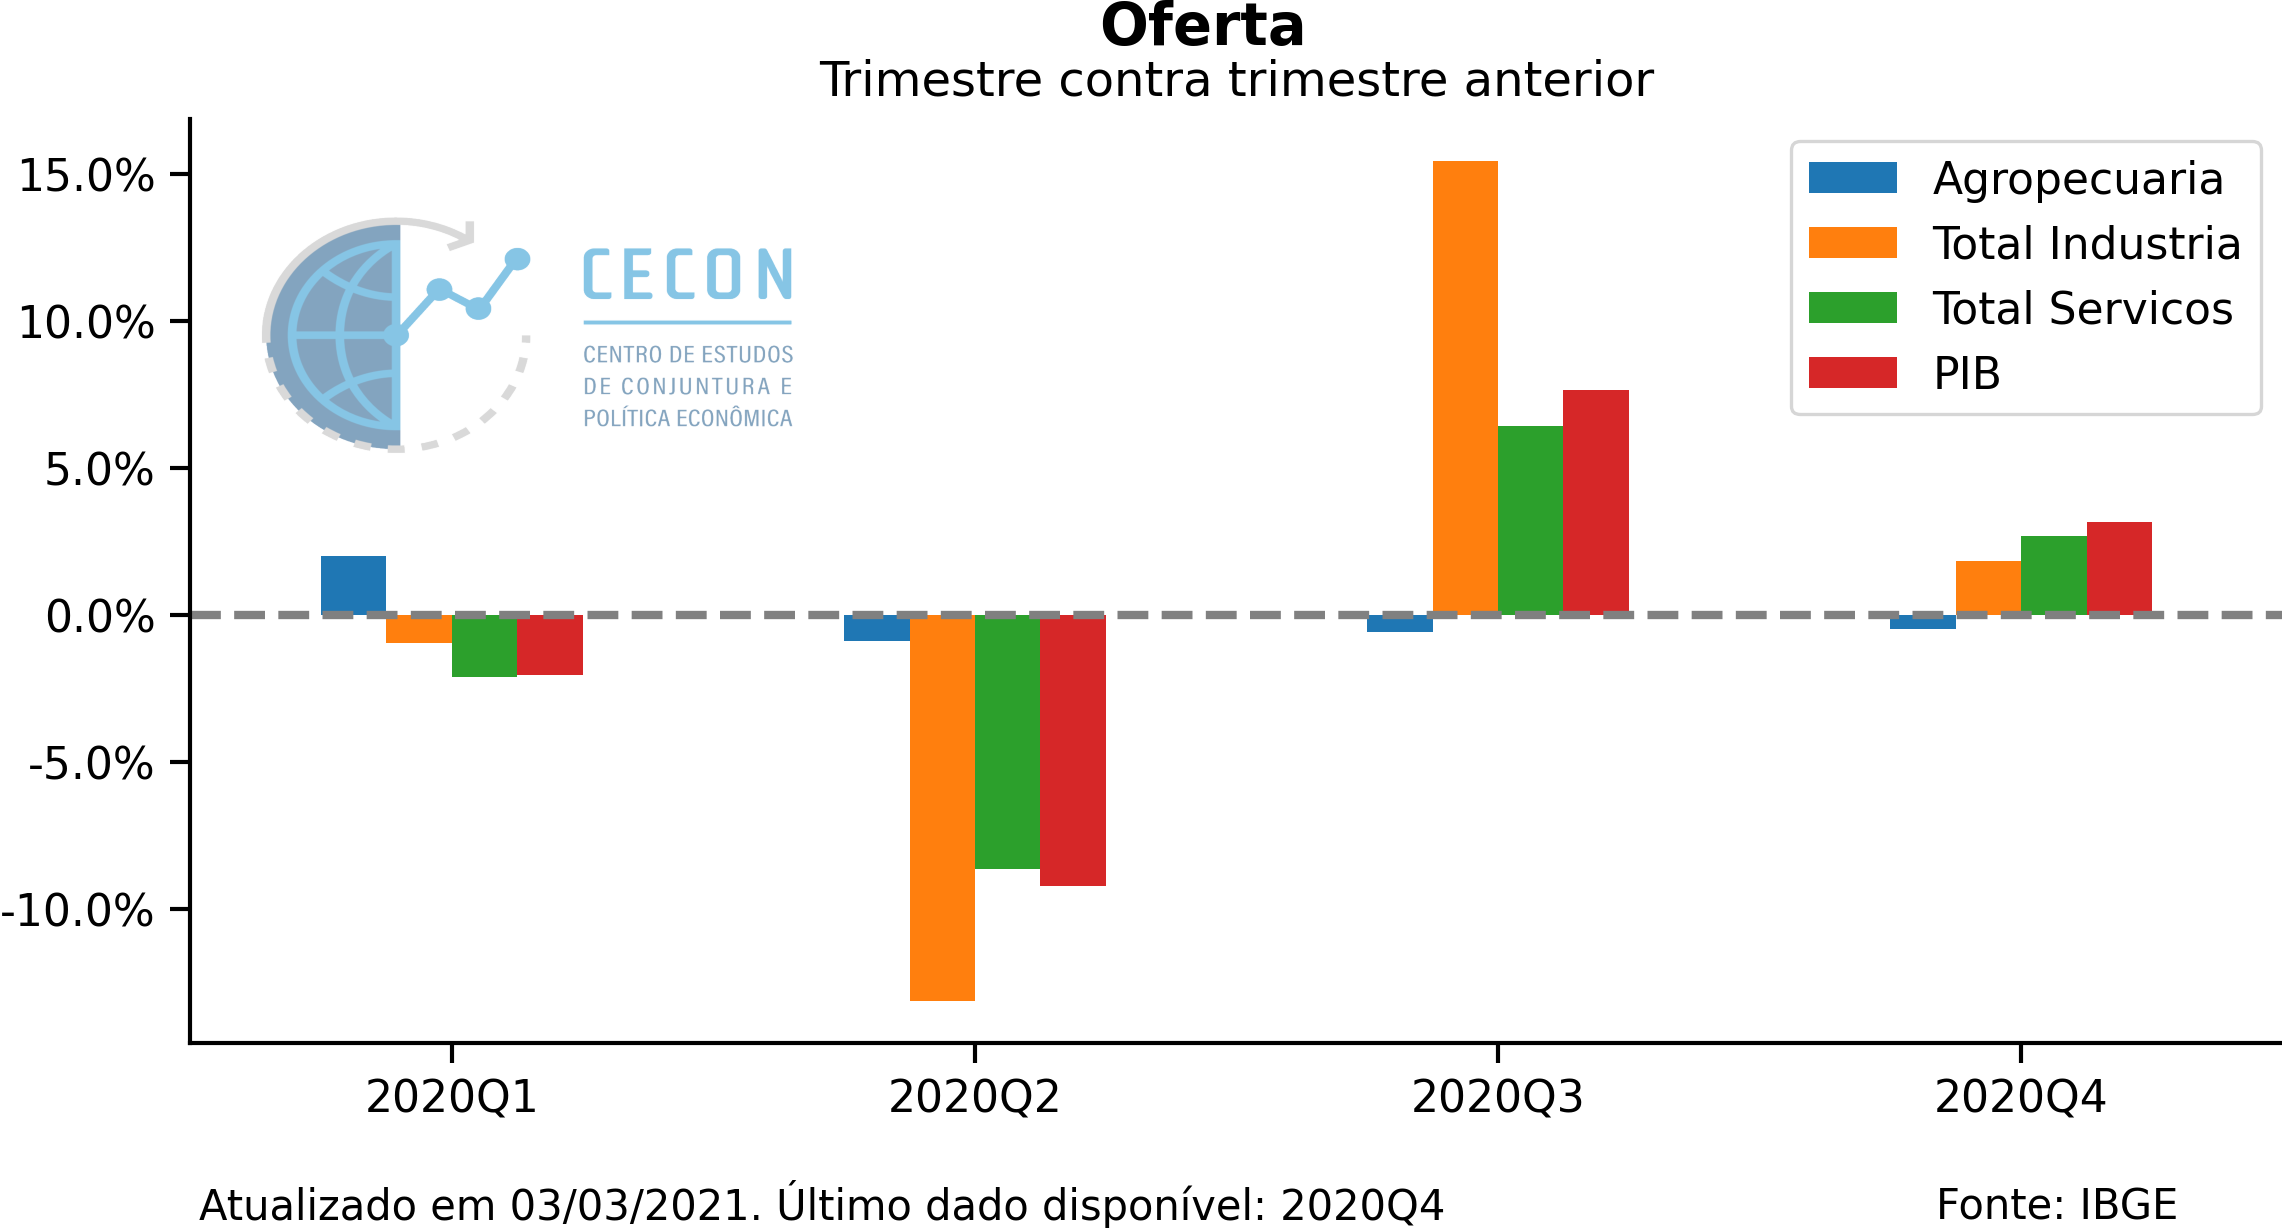
\includegraphics[width=.9\linewidth]{./figs/PIB/Oferta.png}
\end{center}


\subsection*{Contribuição para variação: Demanda}
\label{sec:orgfbcb72a}

\begin{center}
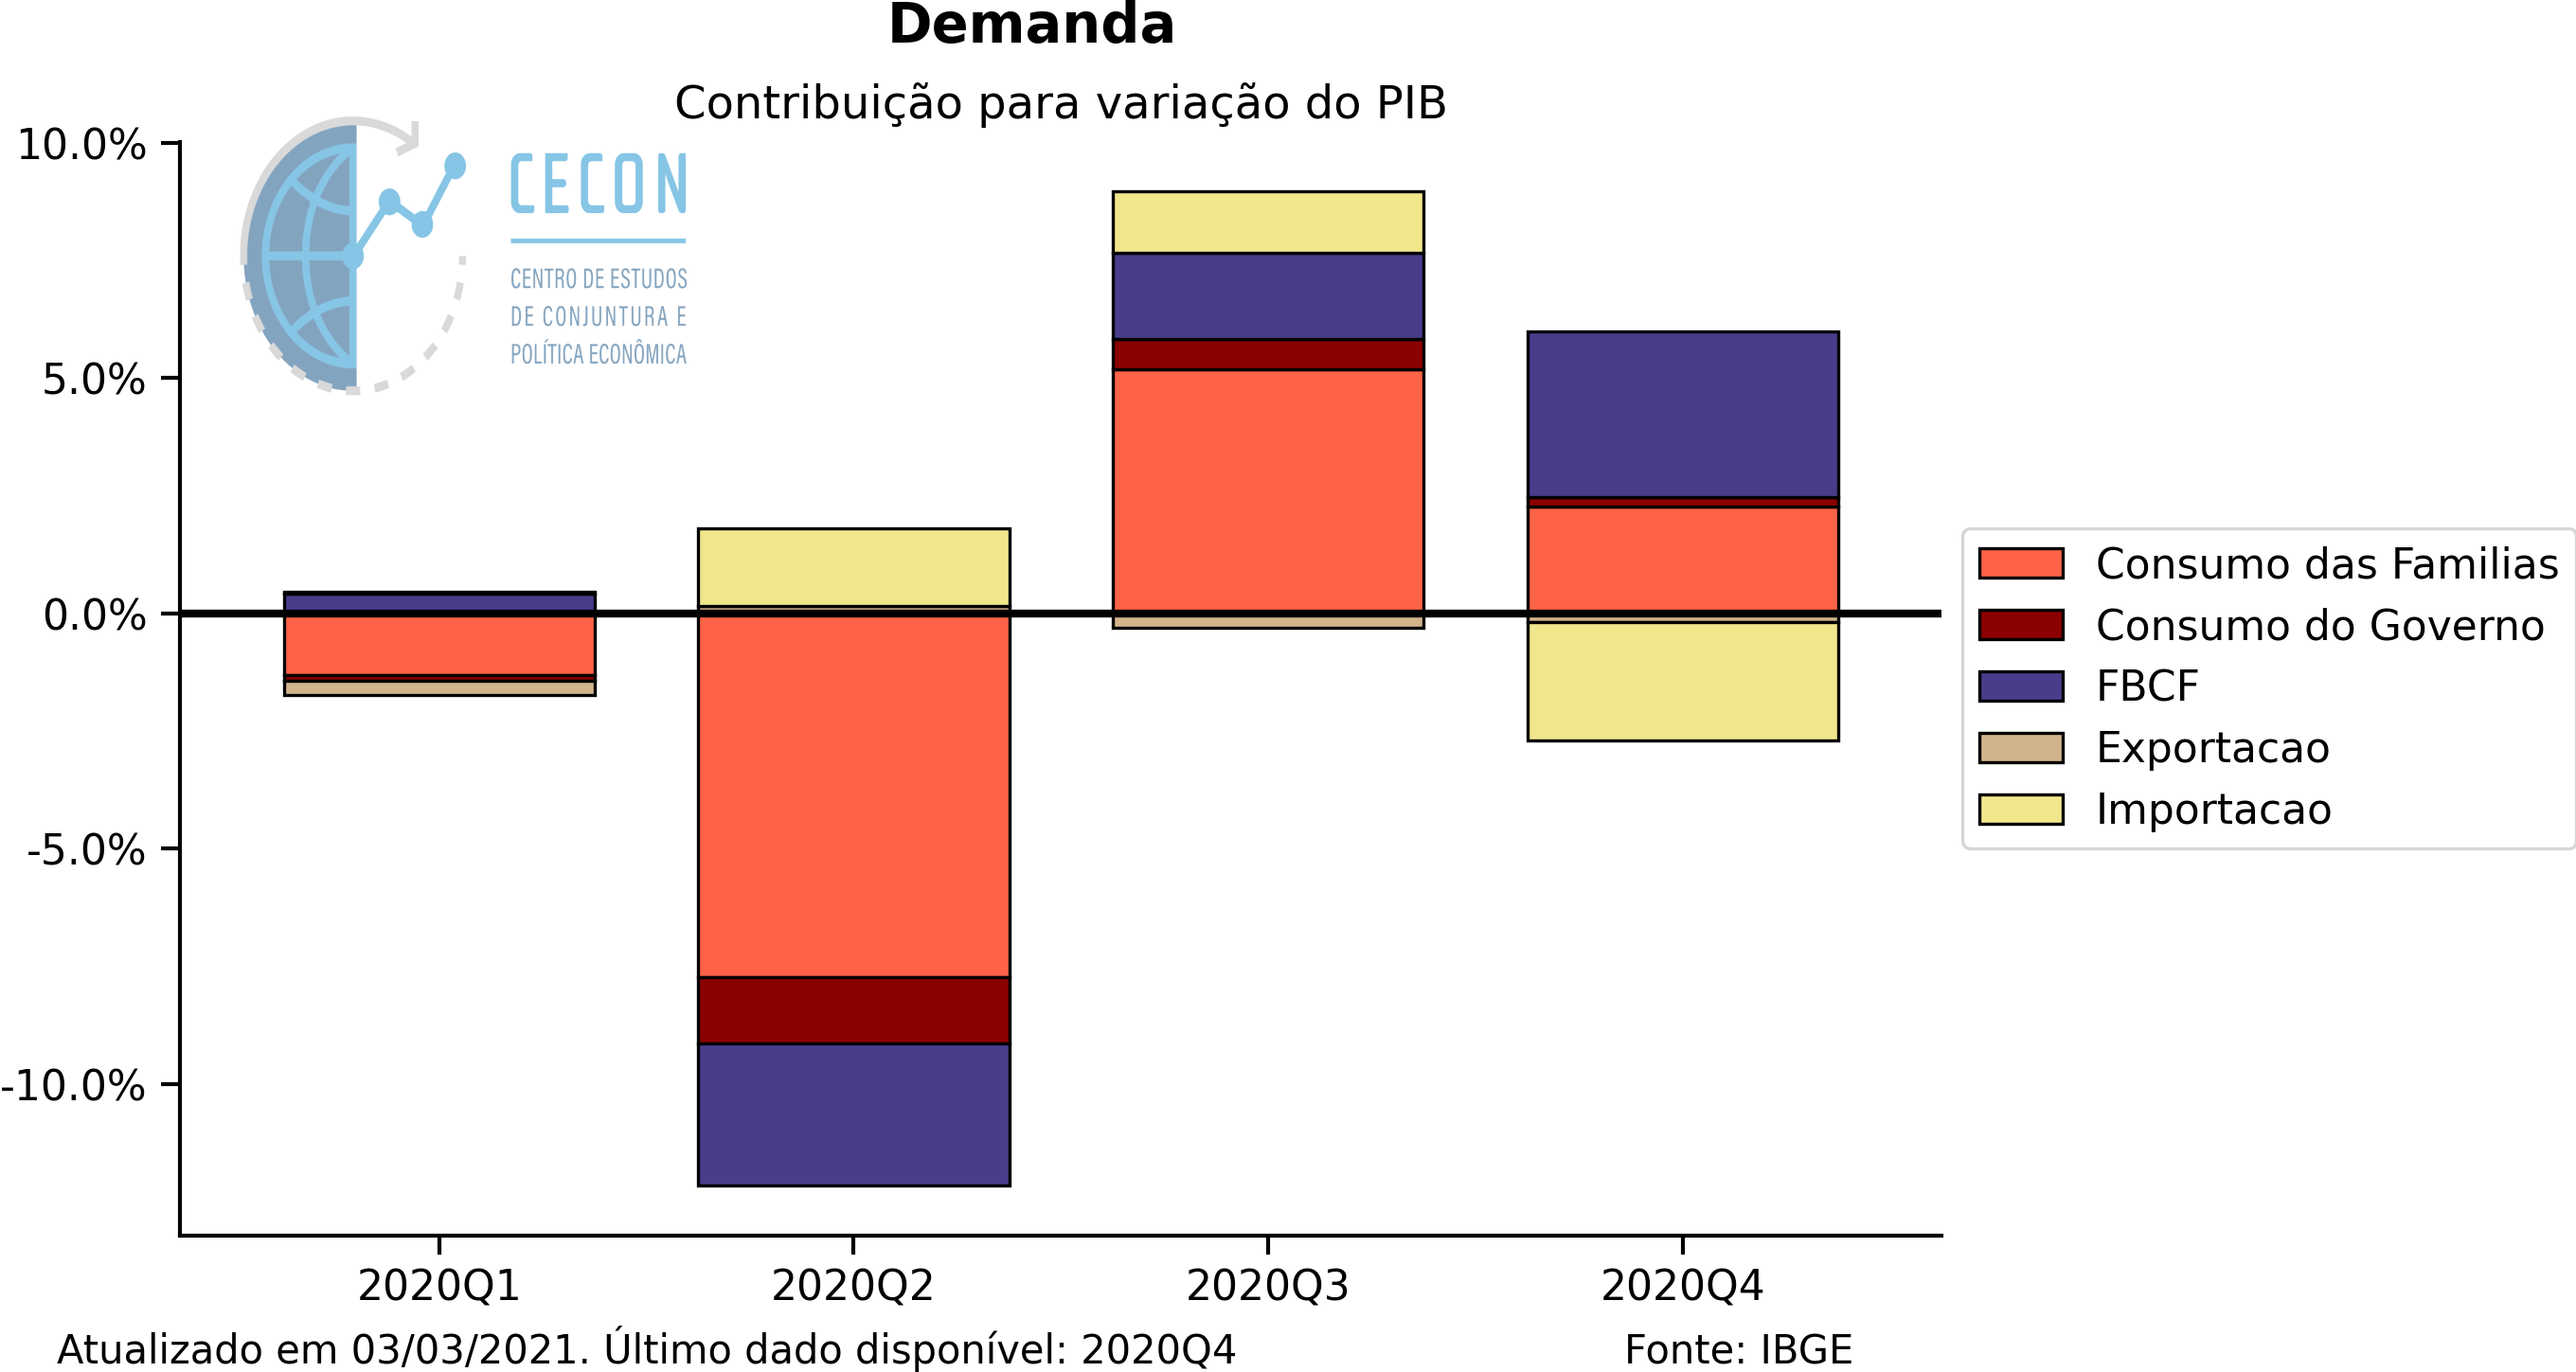
\includegraphics[width=.9\linewidth]{./figs/PIB/Contrib_Demanda.png}
\end{center}

\subsection*{Contribuição para variação: Oferta}
\label{sec:org5b084b3}

\begin{center}
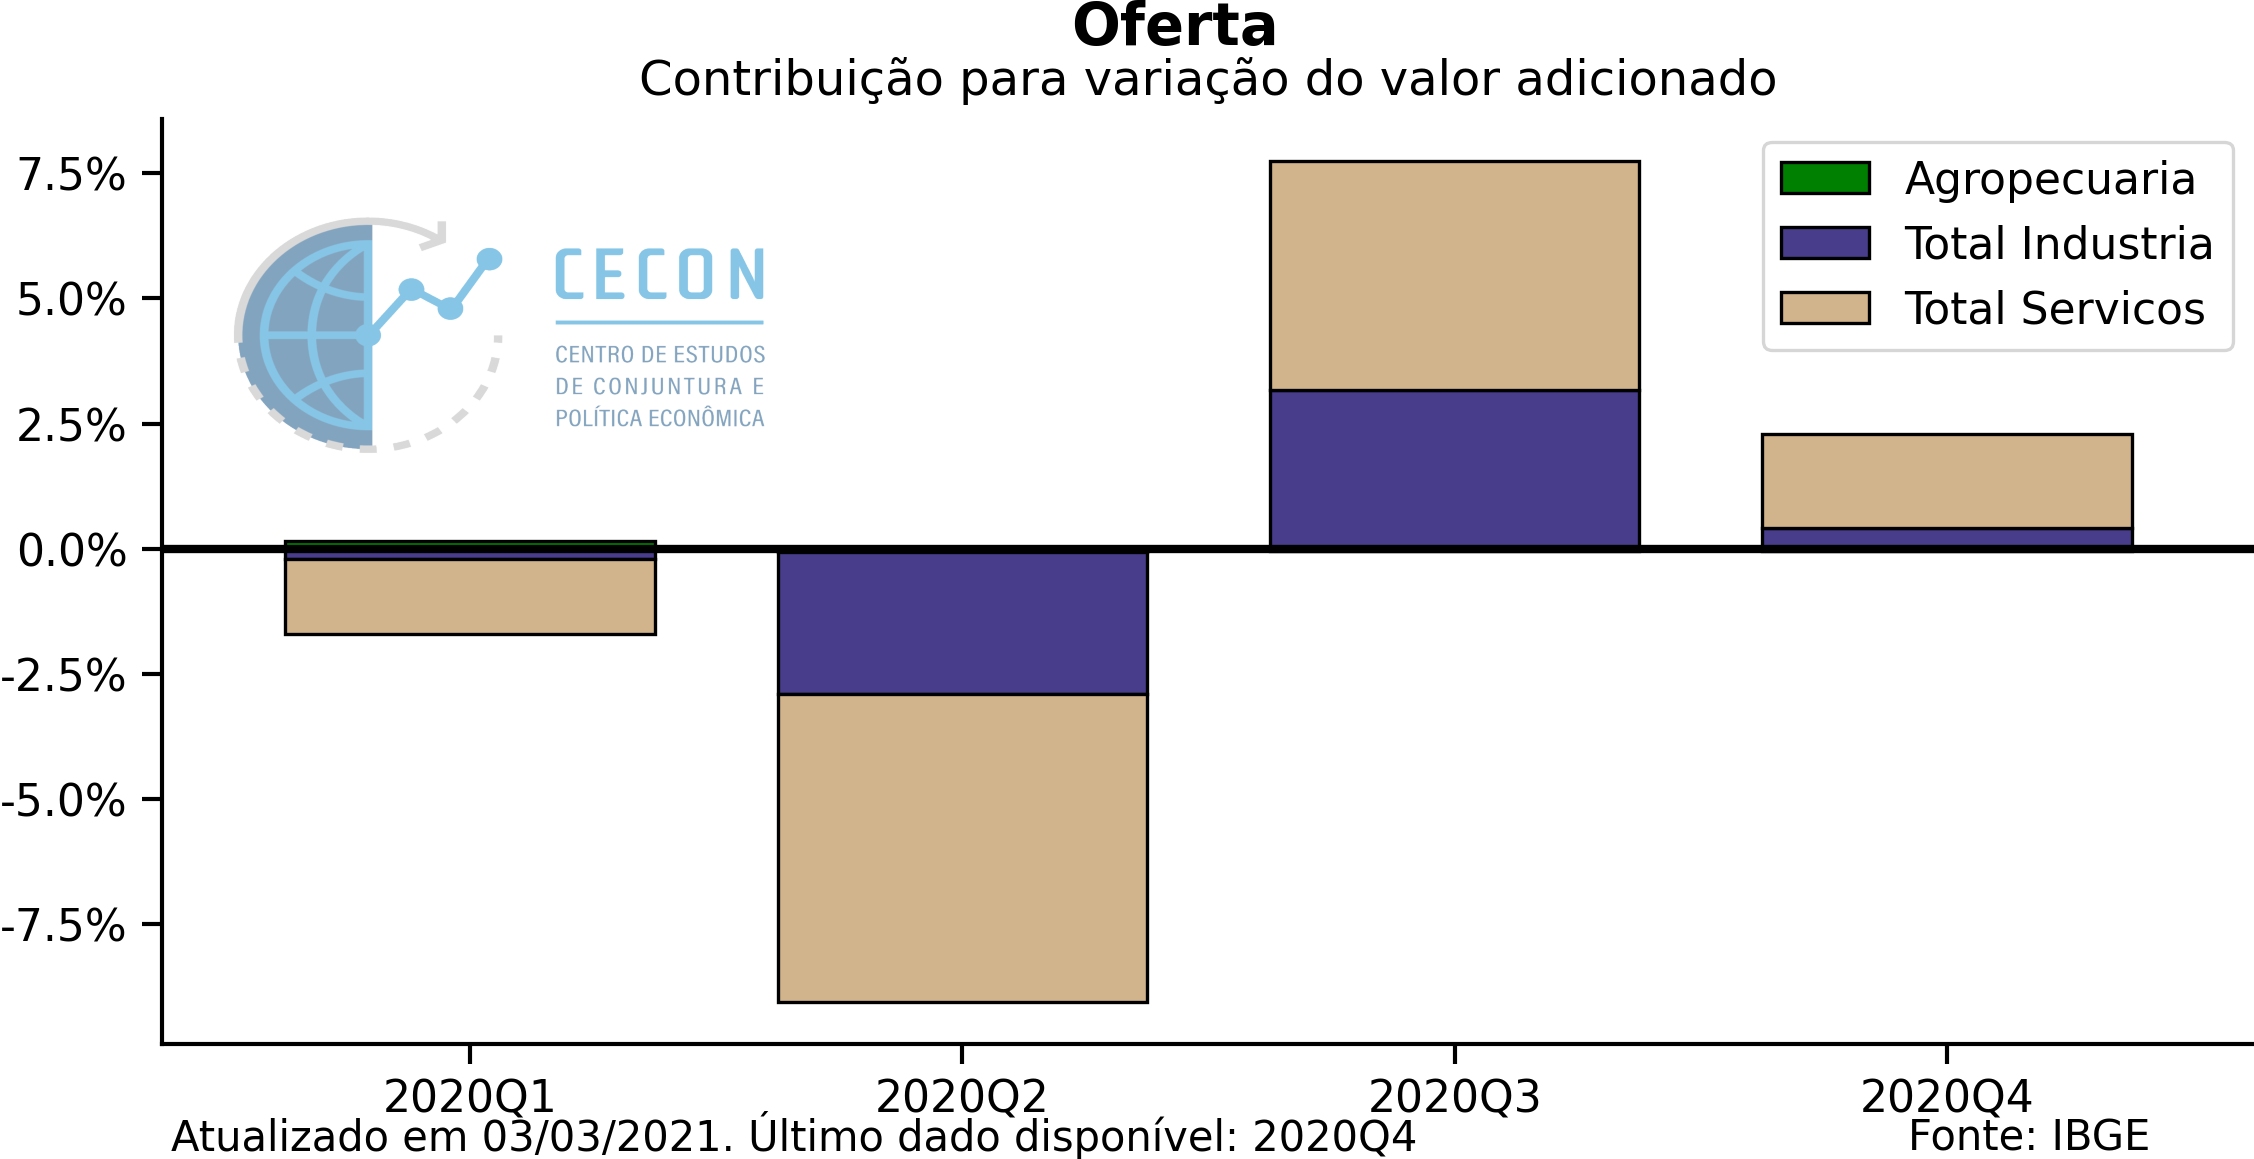
\includegraphics[width=.9\linewidth]{./figs/PIB/Contrib_Oferta.png}
\end{center}


\subsection*{Contribuição para variação: Serviços}
\label{sec:org61ac152}

\begin{center}
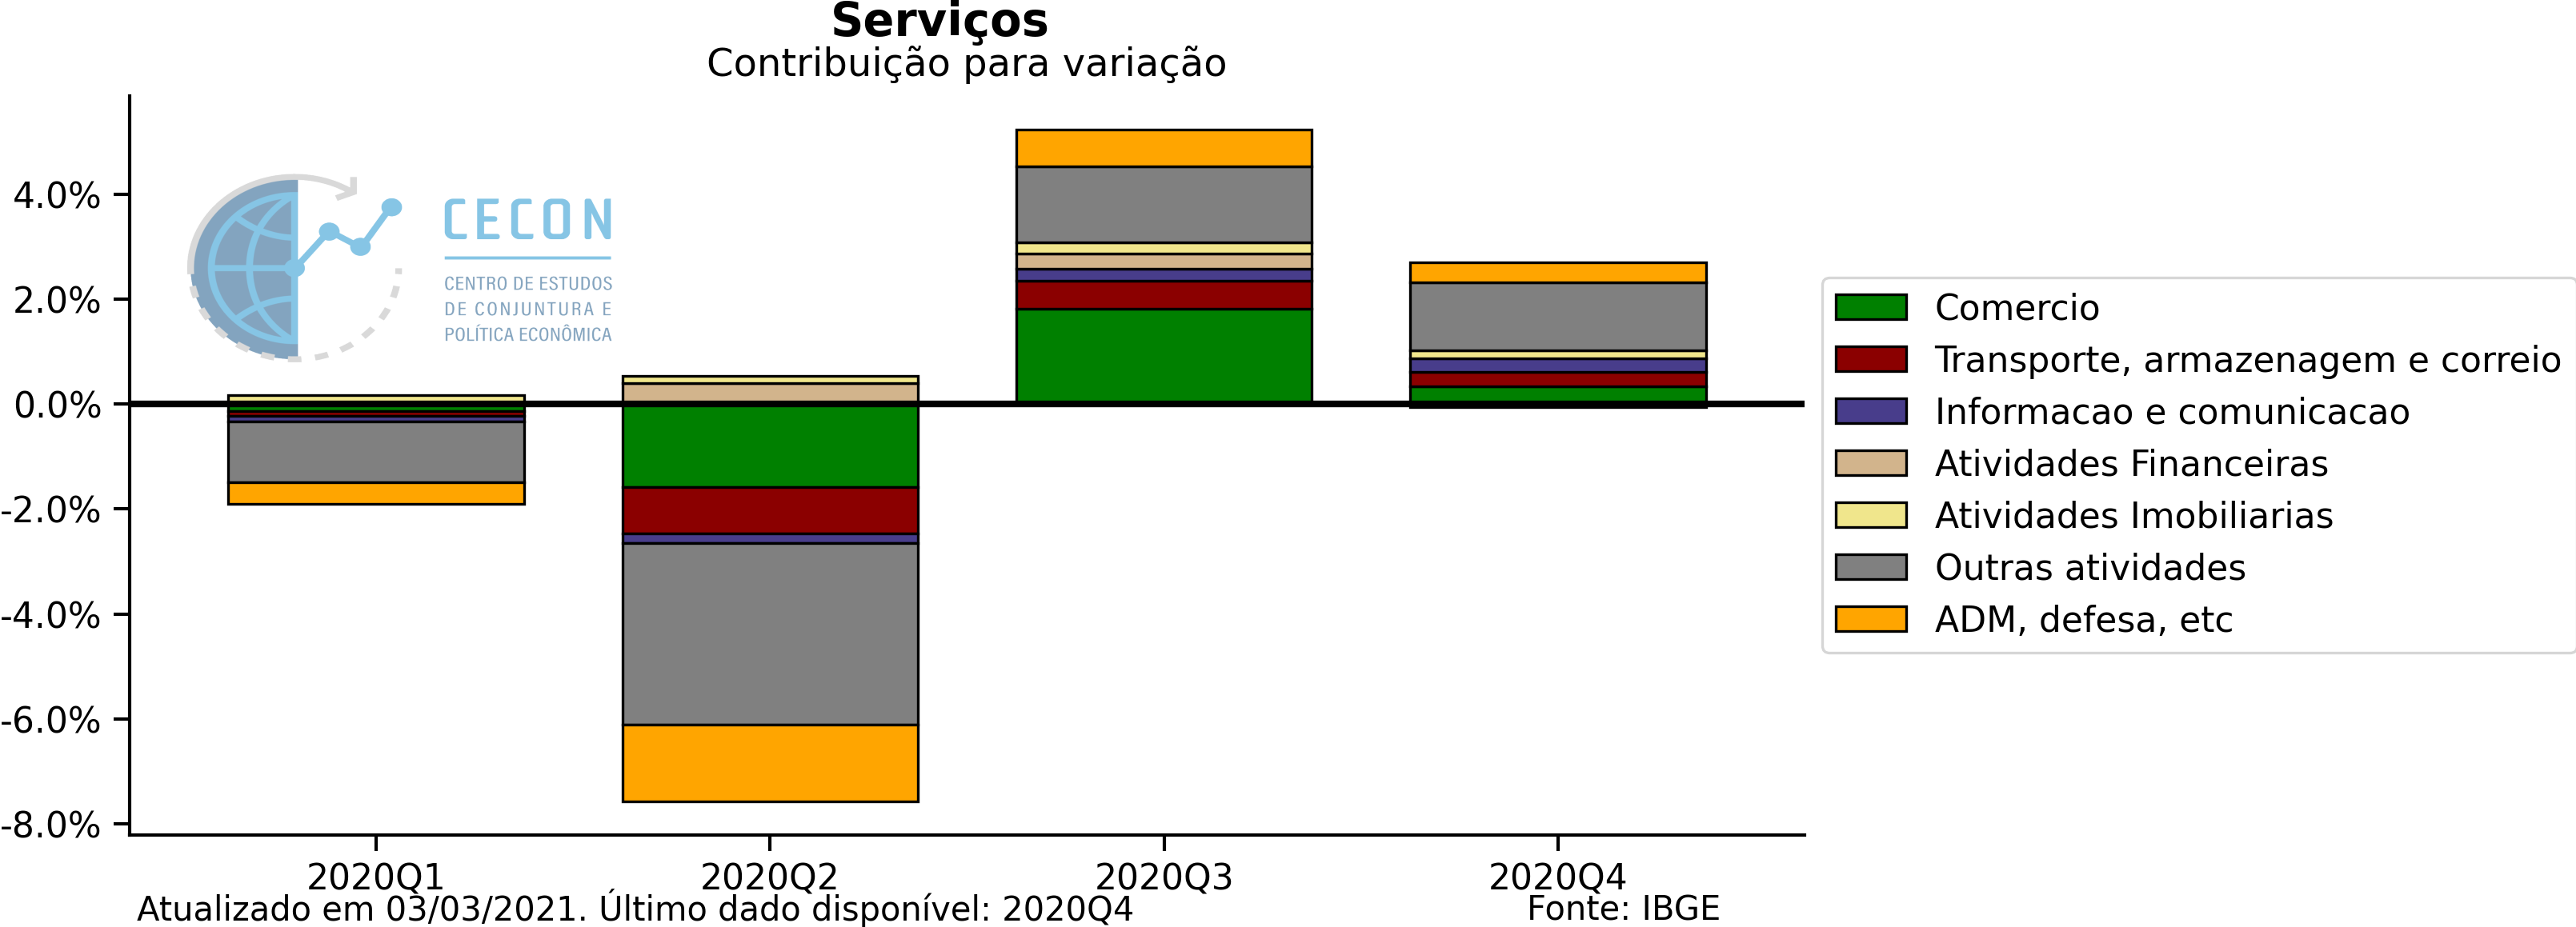
\includegraphics[width=.9\linewidth]{./figs/PIB/Contrib_Servicos.png}
\end{center}

\section*{Crédito}
\label{sec:org6d8d2ef}

\subsection*{Endividamento das famílias}
\label{sec:org3b30d32}

\begin{center}
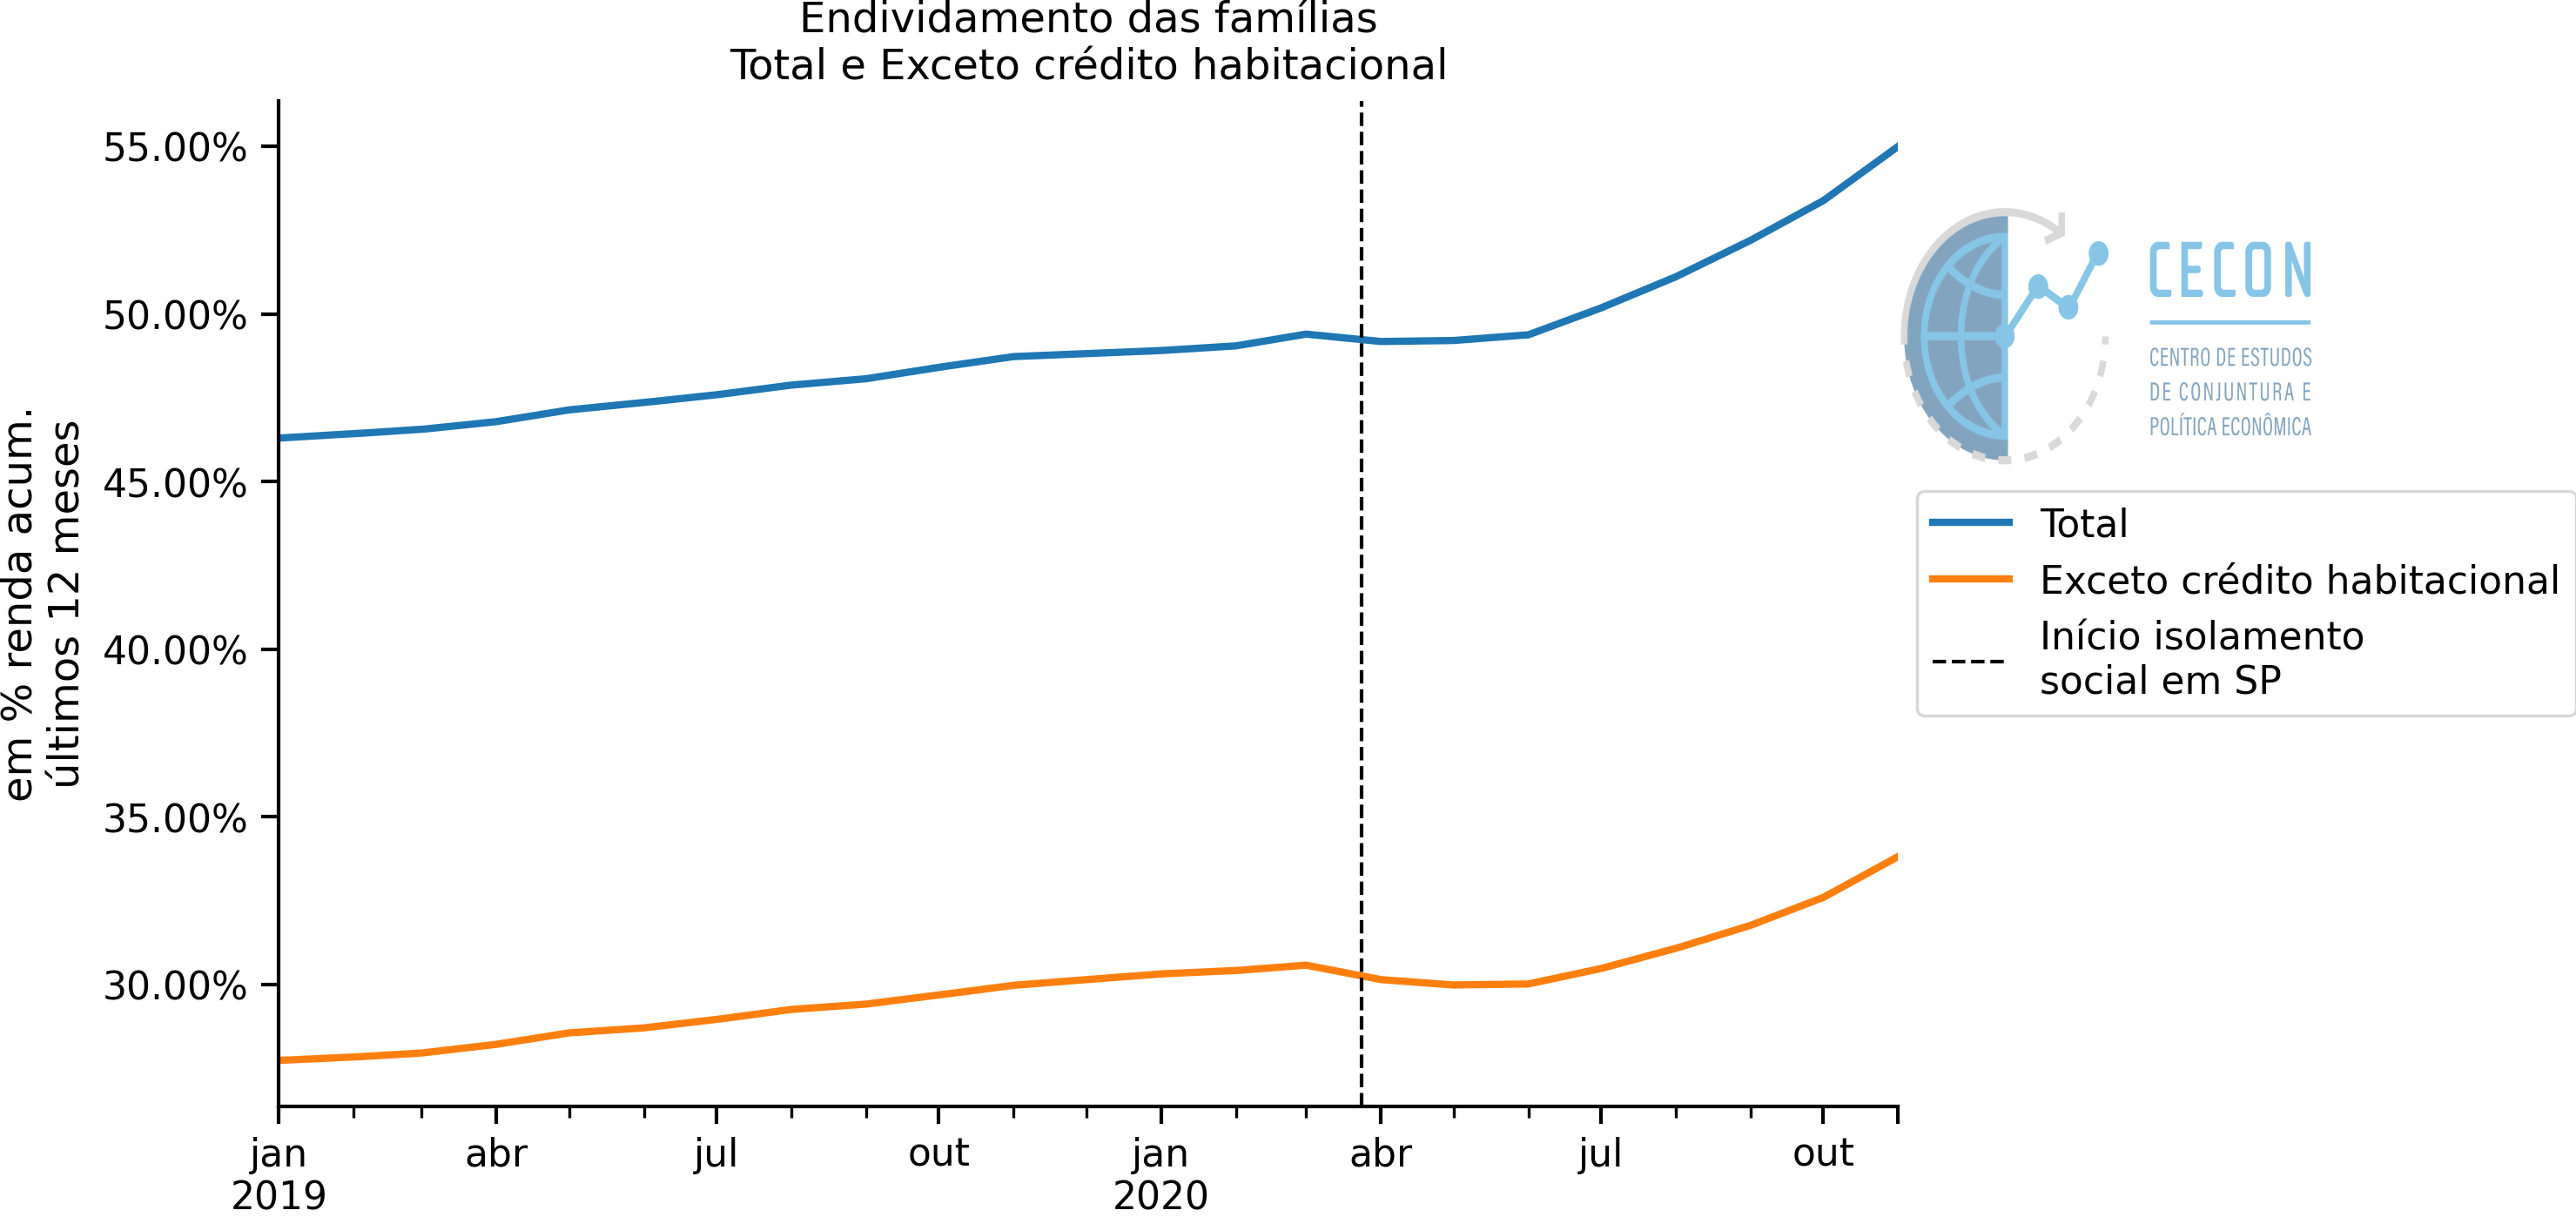
\includegraphics[width=.9\linewidth]{./figs/Credito/EndividamentoFamilias.png}
\end{center}


\subsection*{Saldo Pessoal Jurídica - Nível}
\label{sec:org6d715ae}

\begin{center}
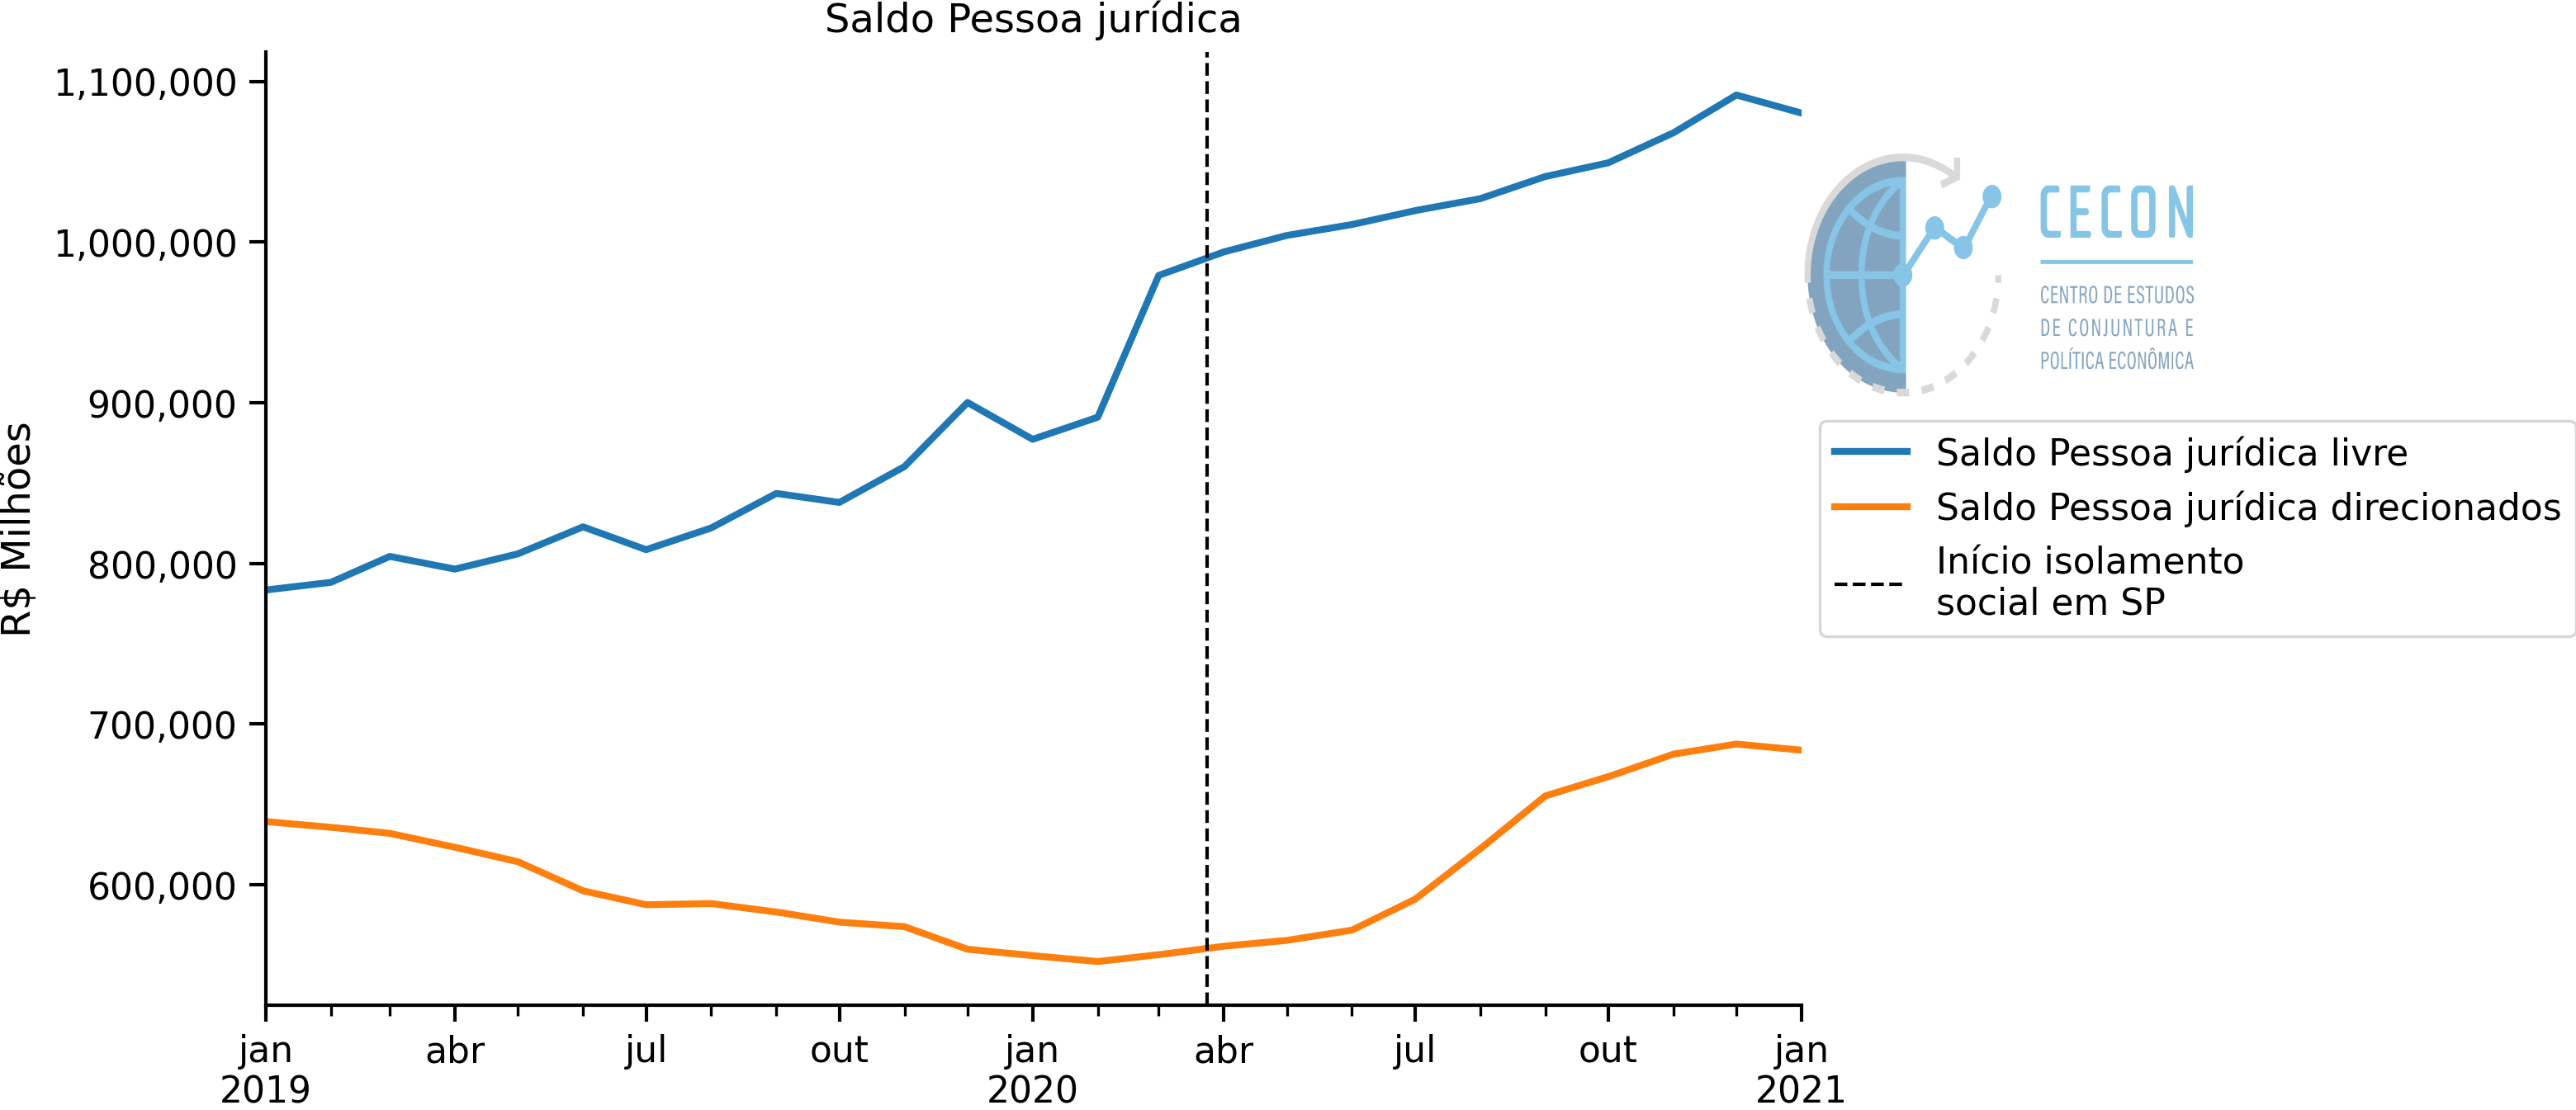
\includegraphics[width=.9\linewidth]{./figs/Credito/SaldoPJ.png}
\end{center}



\subsection*{Saldo Pessoa Jurídica - em \% do PIB}
\label{sec:org5c6672d}
\begin{center}
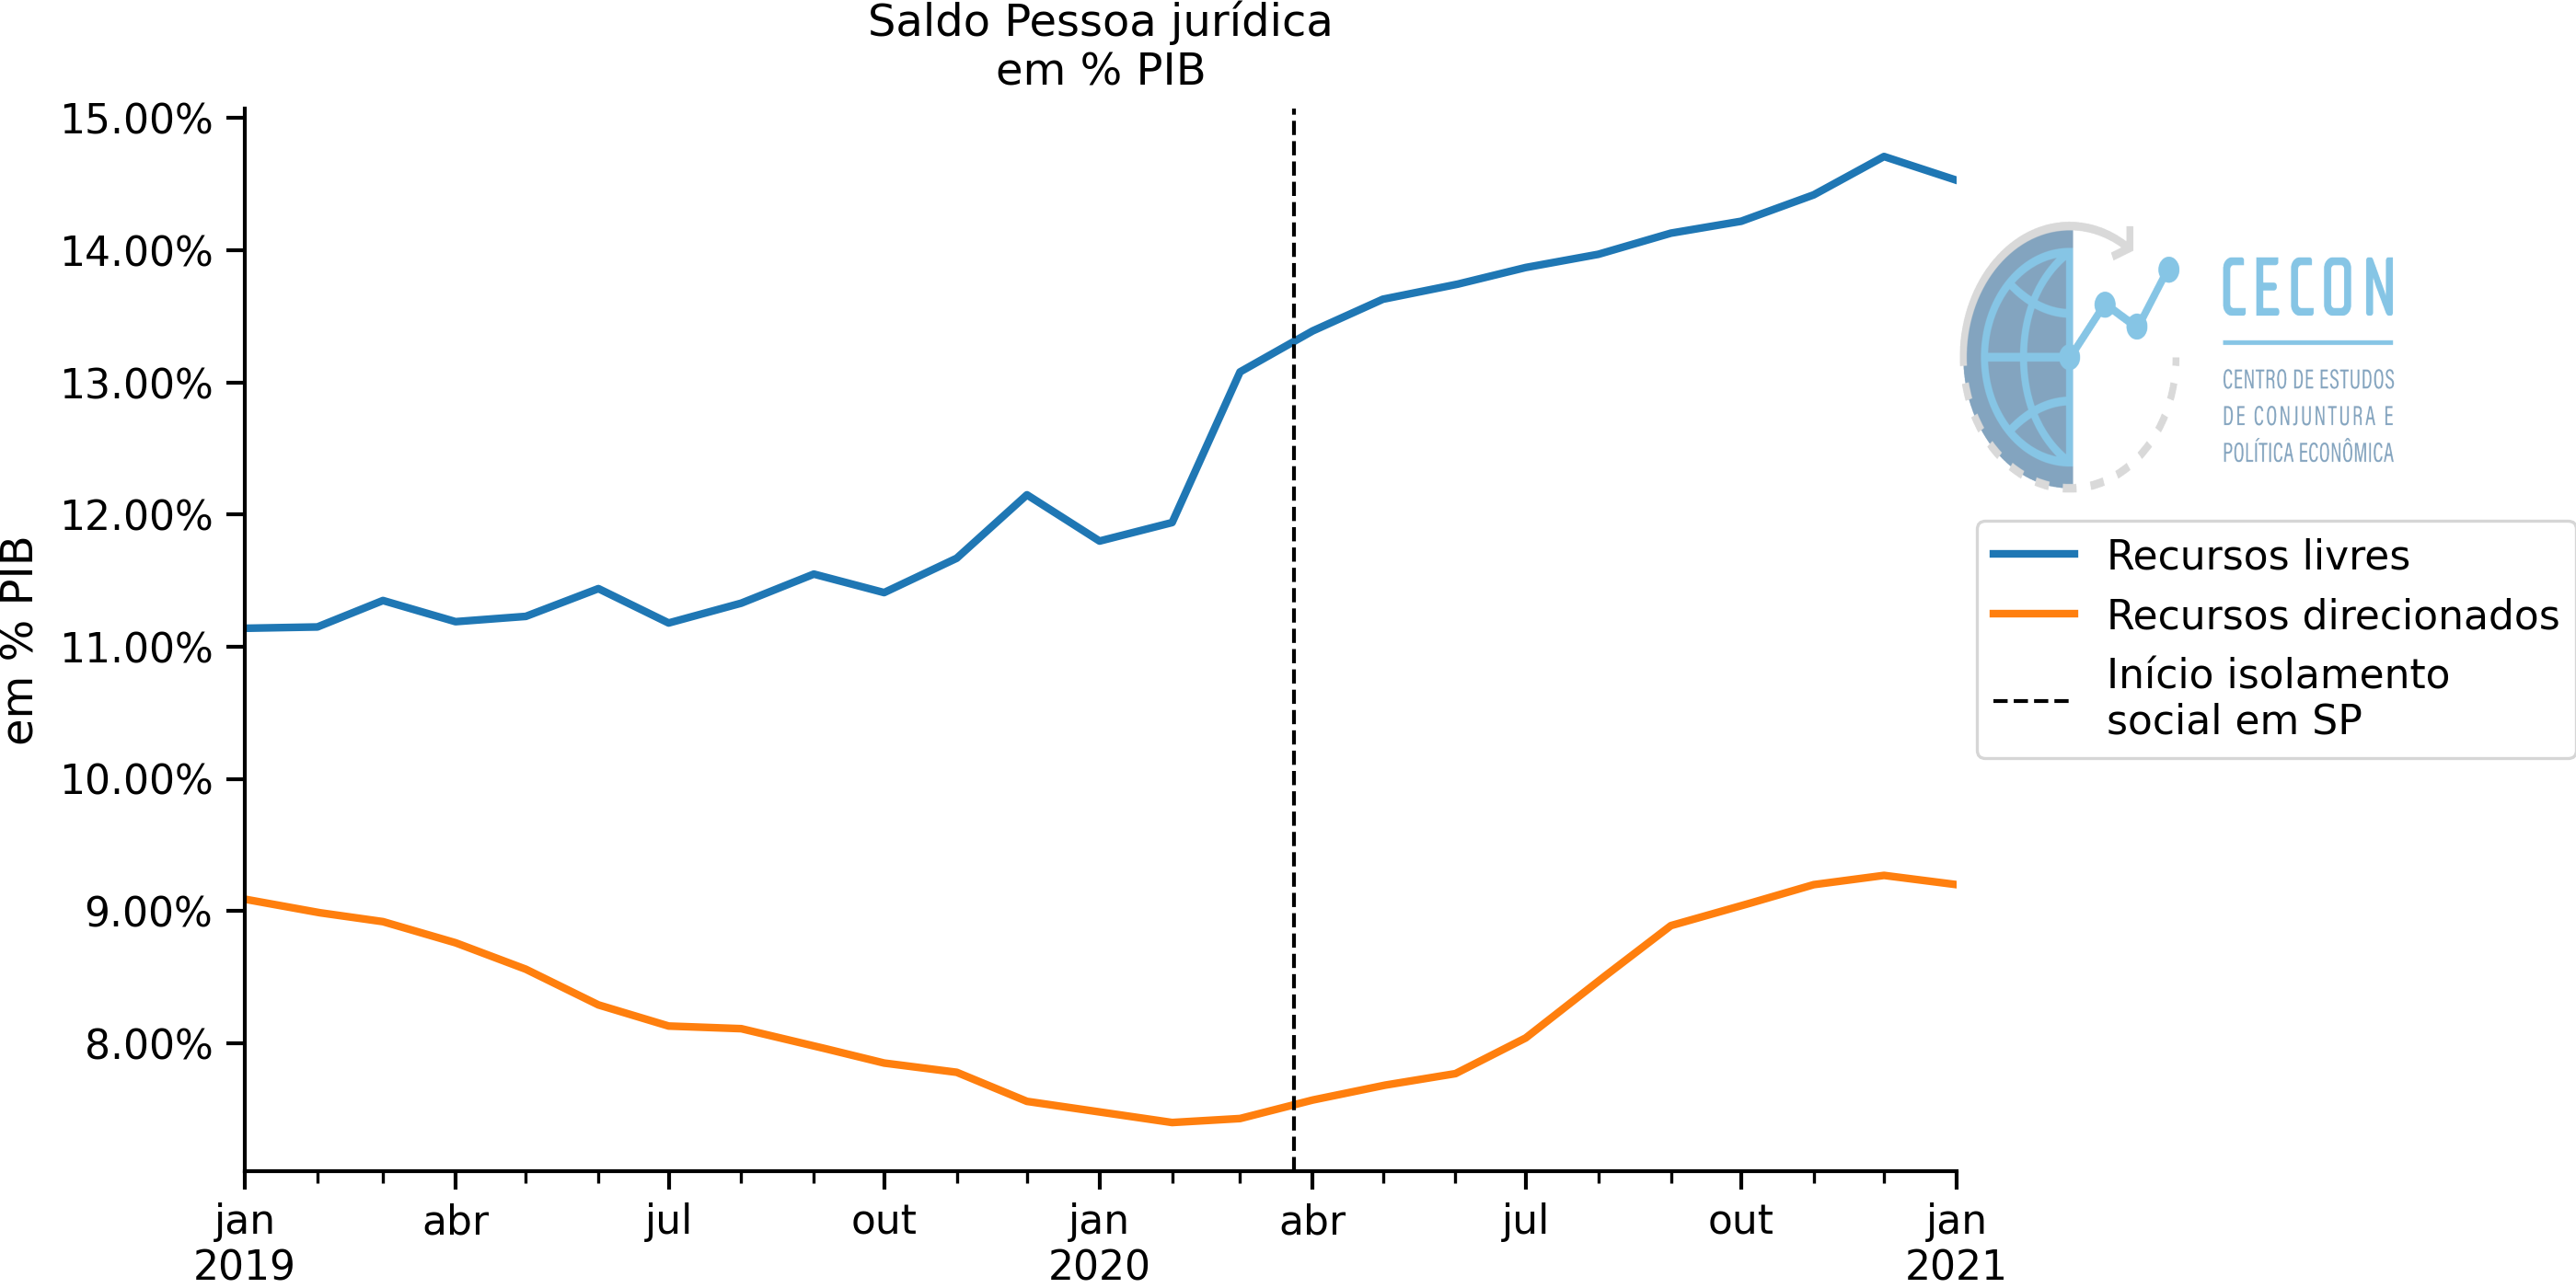
\includegraphics[width=.9\linewidth]{./figs/Credito/SaldoPJ_PIB.png}
\end{center}

\subsection*{Saldo Pessoa física - Nível}
\label{sec:org52d7456}

\begin{center}
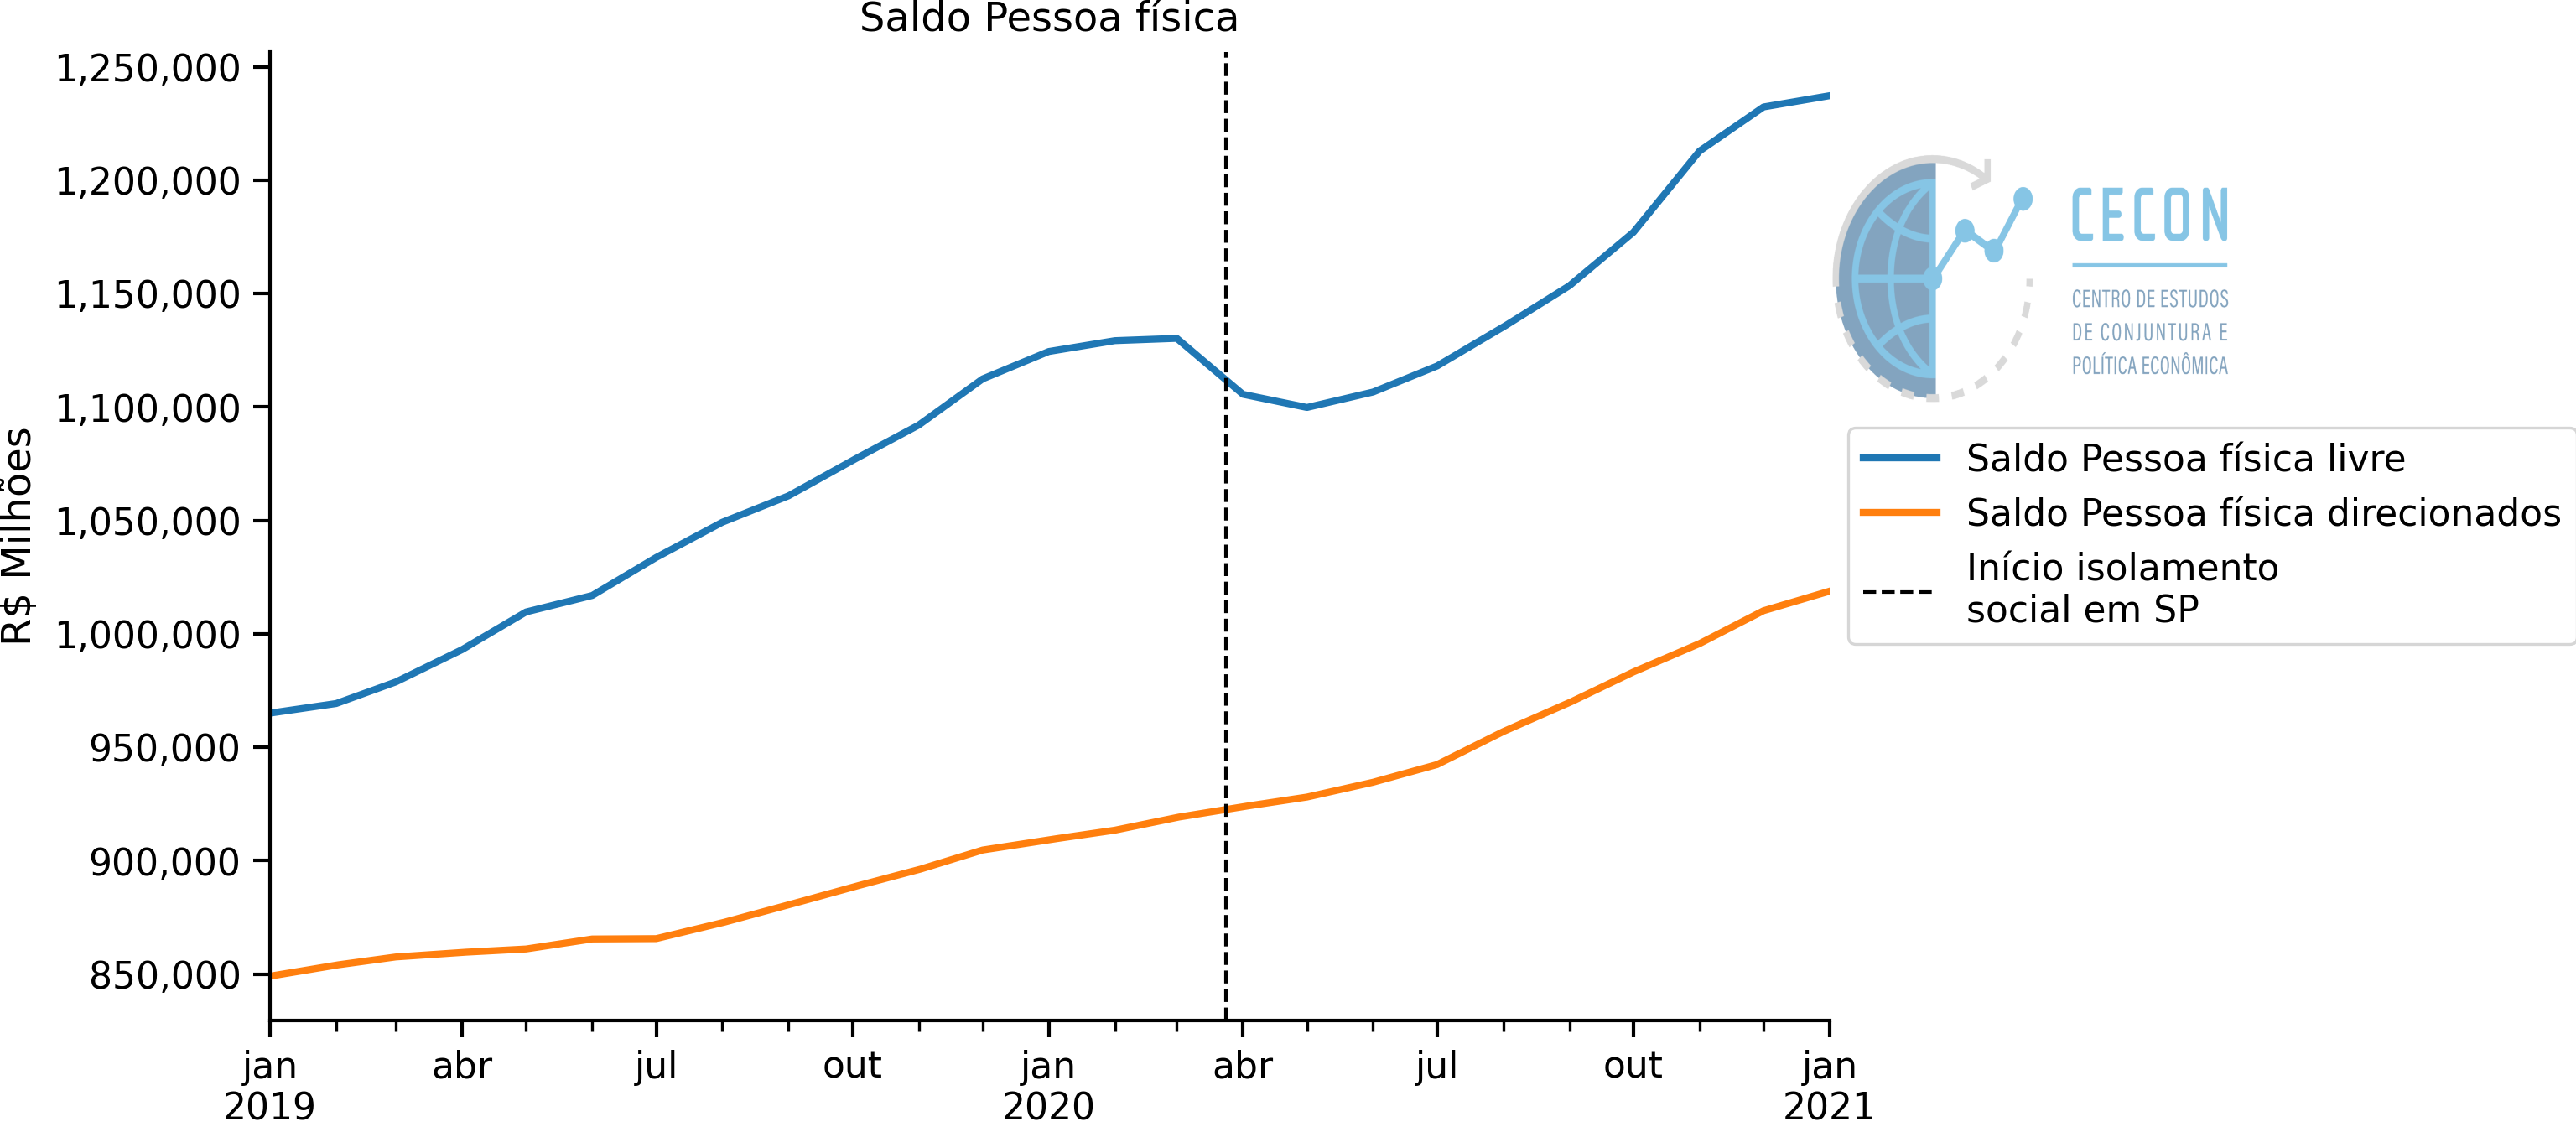
\includegraphics[width=.9\linewidth]{./figs/Credito/SaldoPF.png}
\end{center}


\subsection*{Saldo Pessoa física - em \% do PIB}
\label{sec:org5b9feed}

\begin{center}
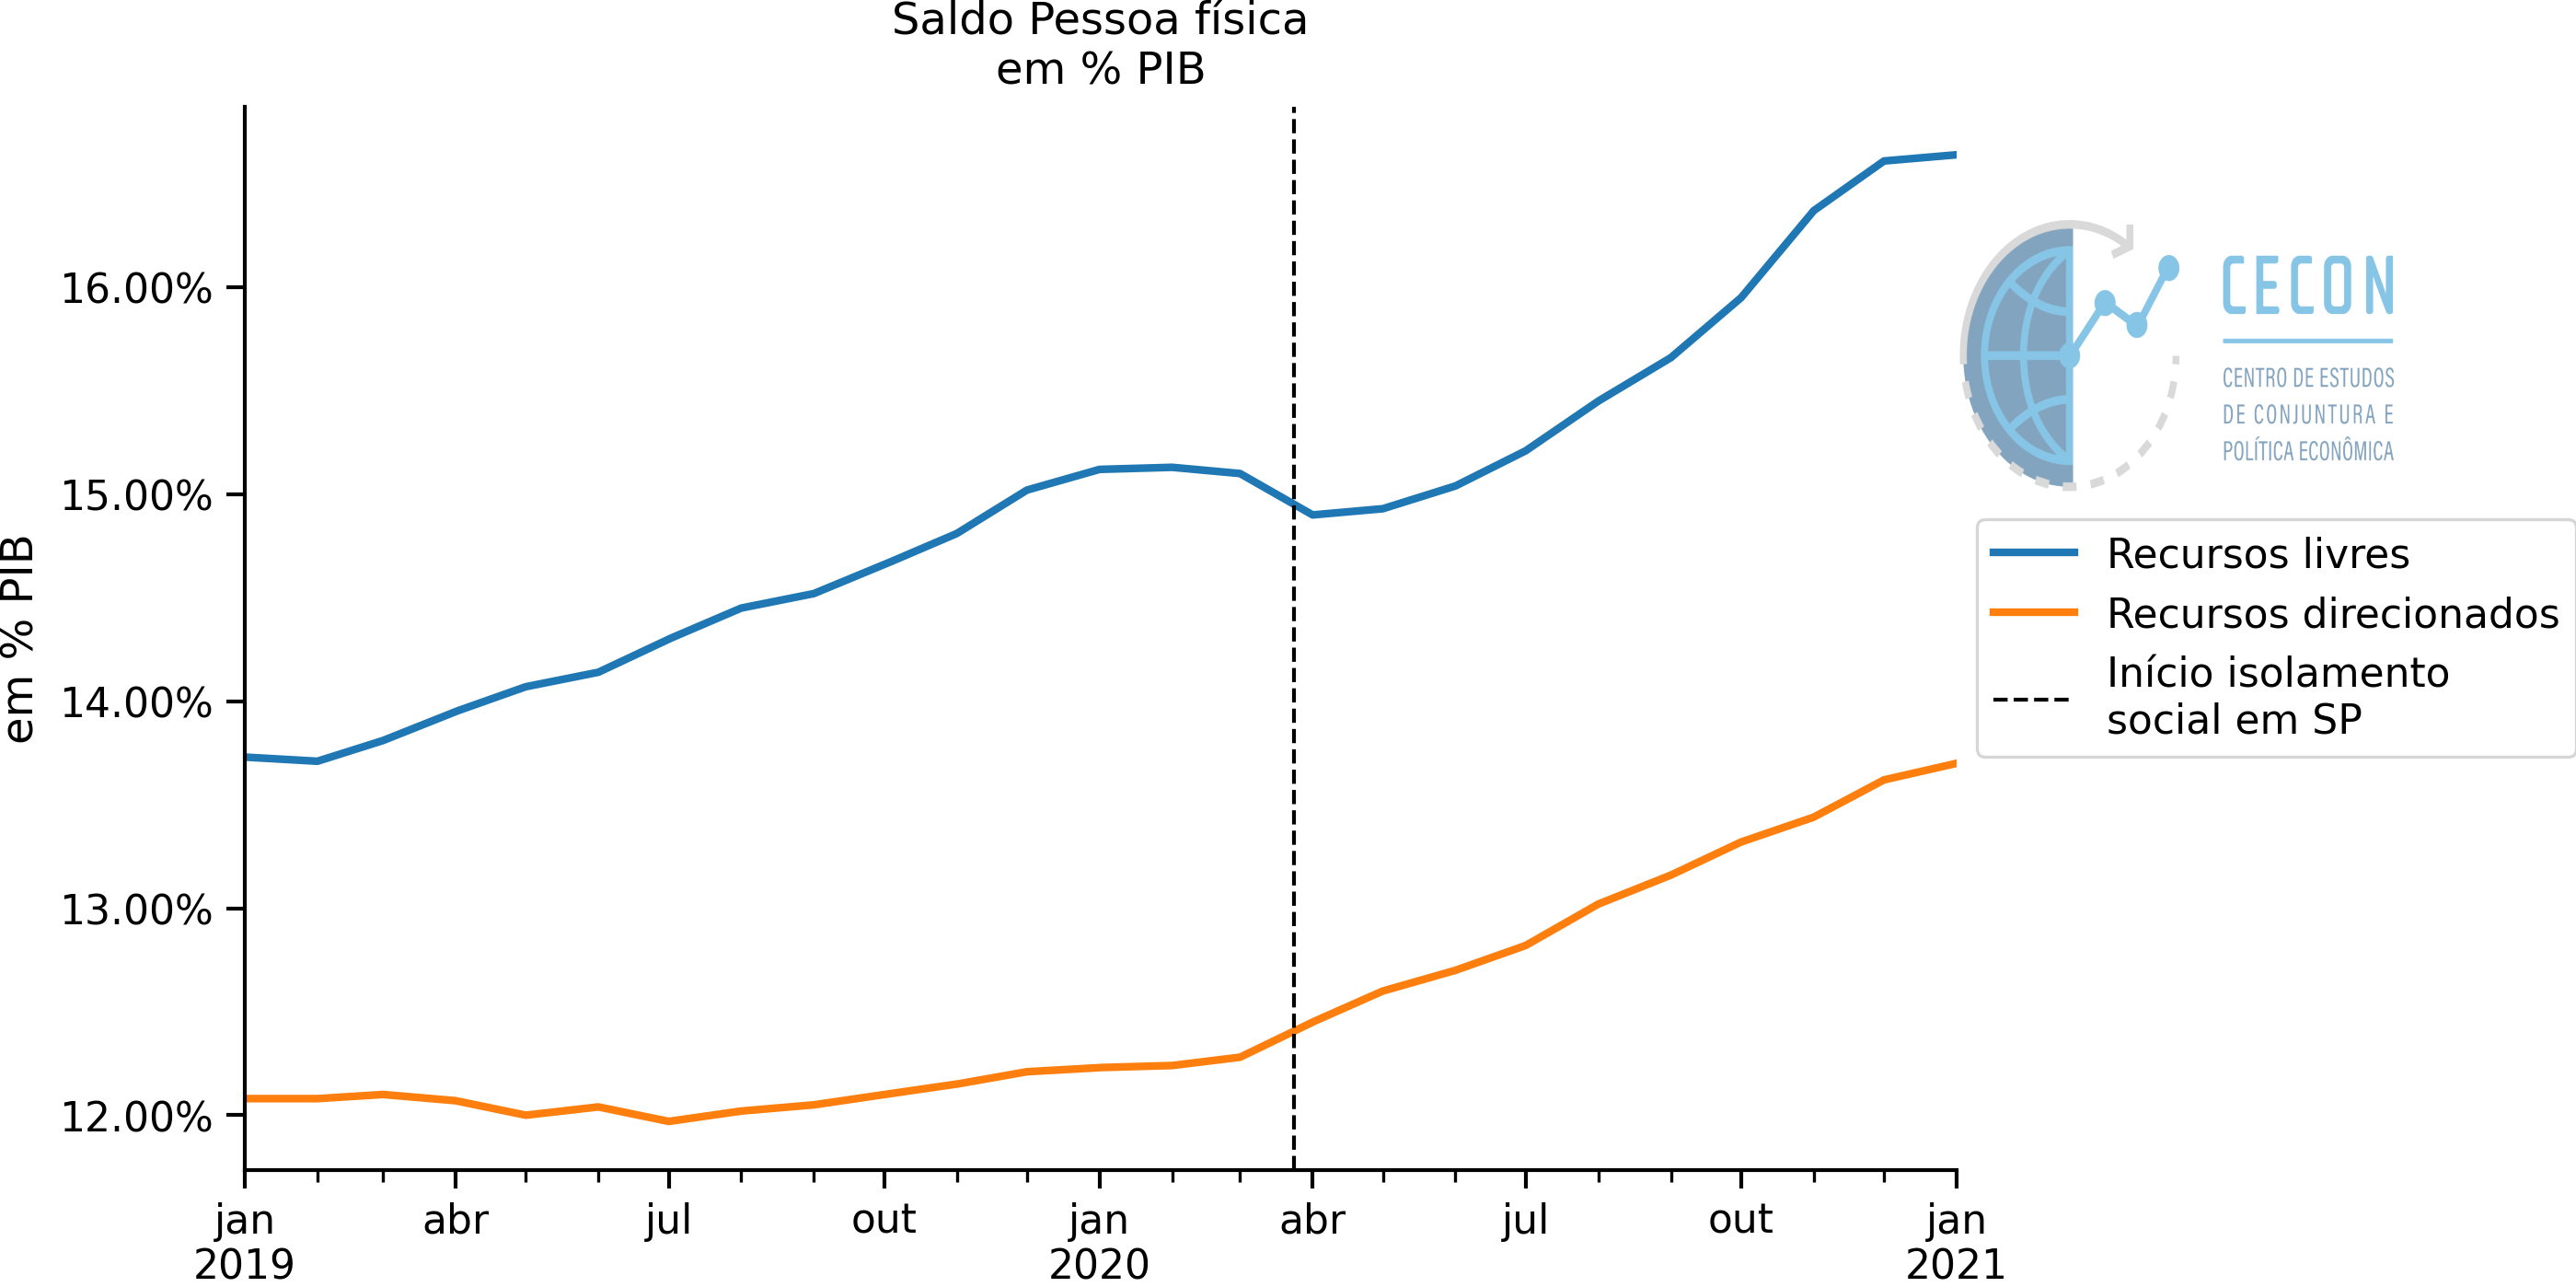
\includegraphics[width=.9\linewidth]{./figs/Credito/SaldoPF_PIB.png}
\end{center}


\subsection*{Crédito ampliado em \% do Total}
\label{sec:org6af6ff0}

\begin{center}
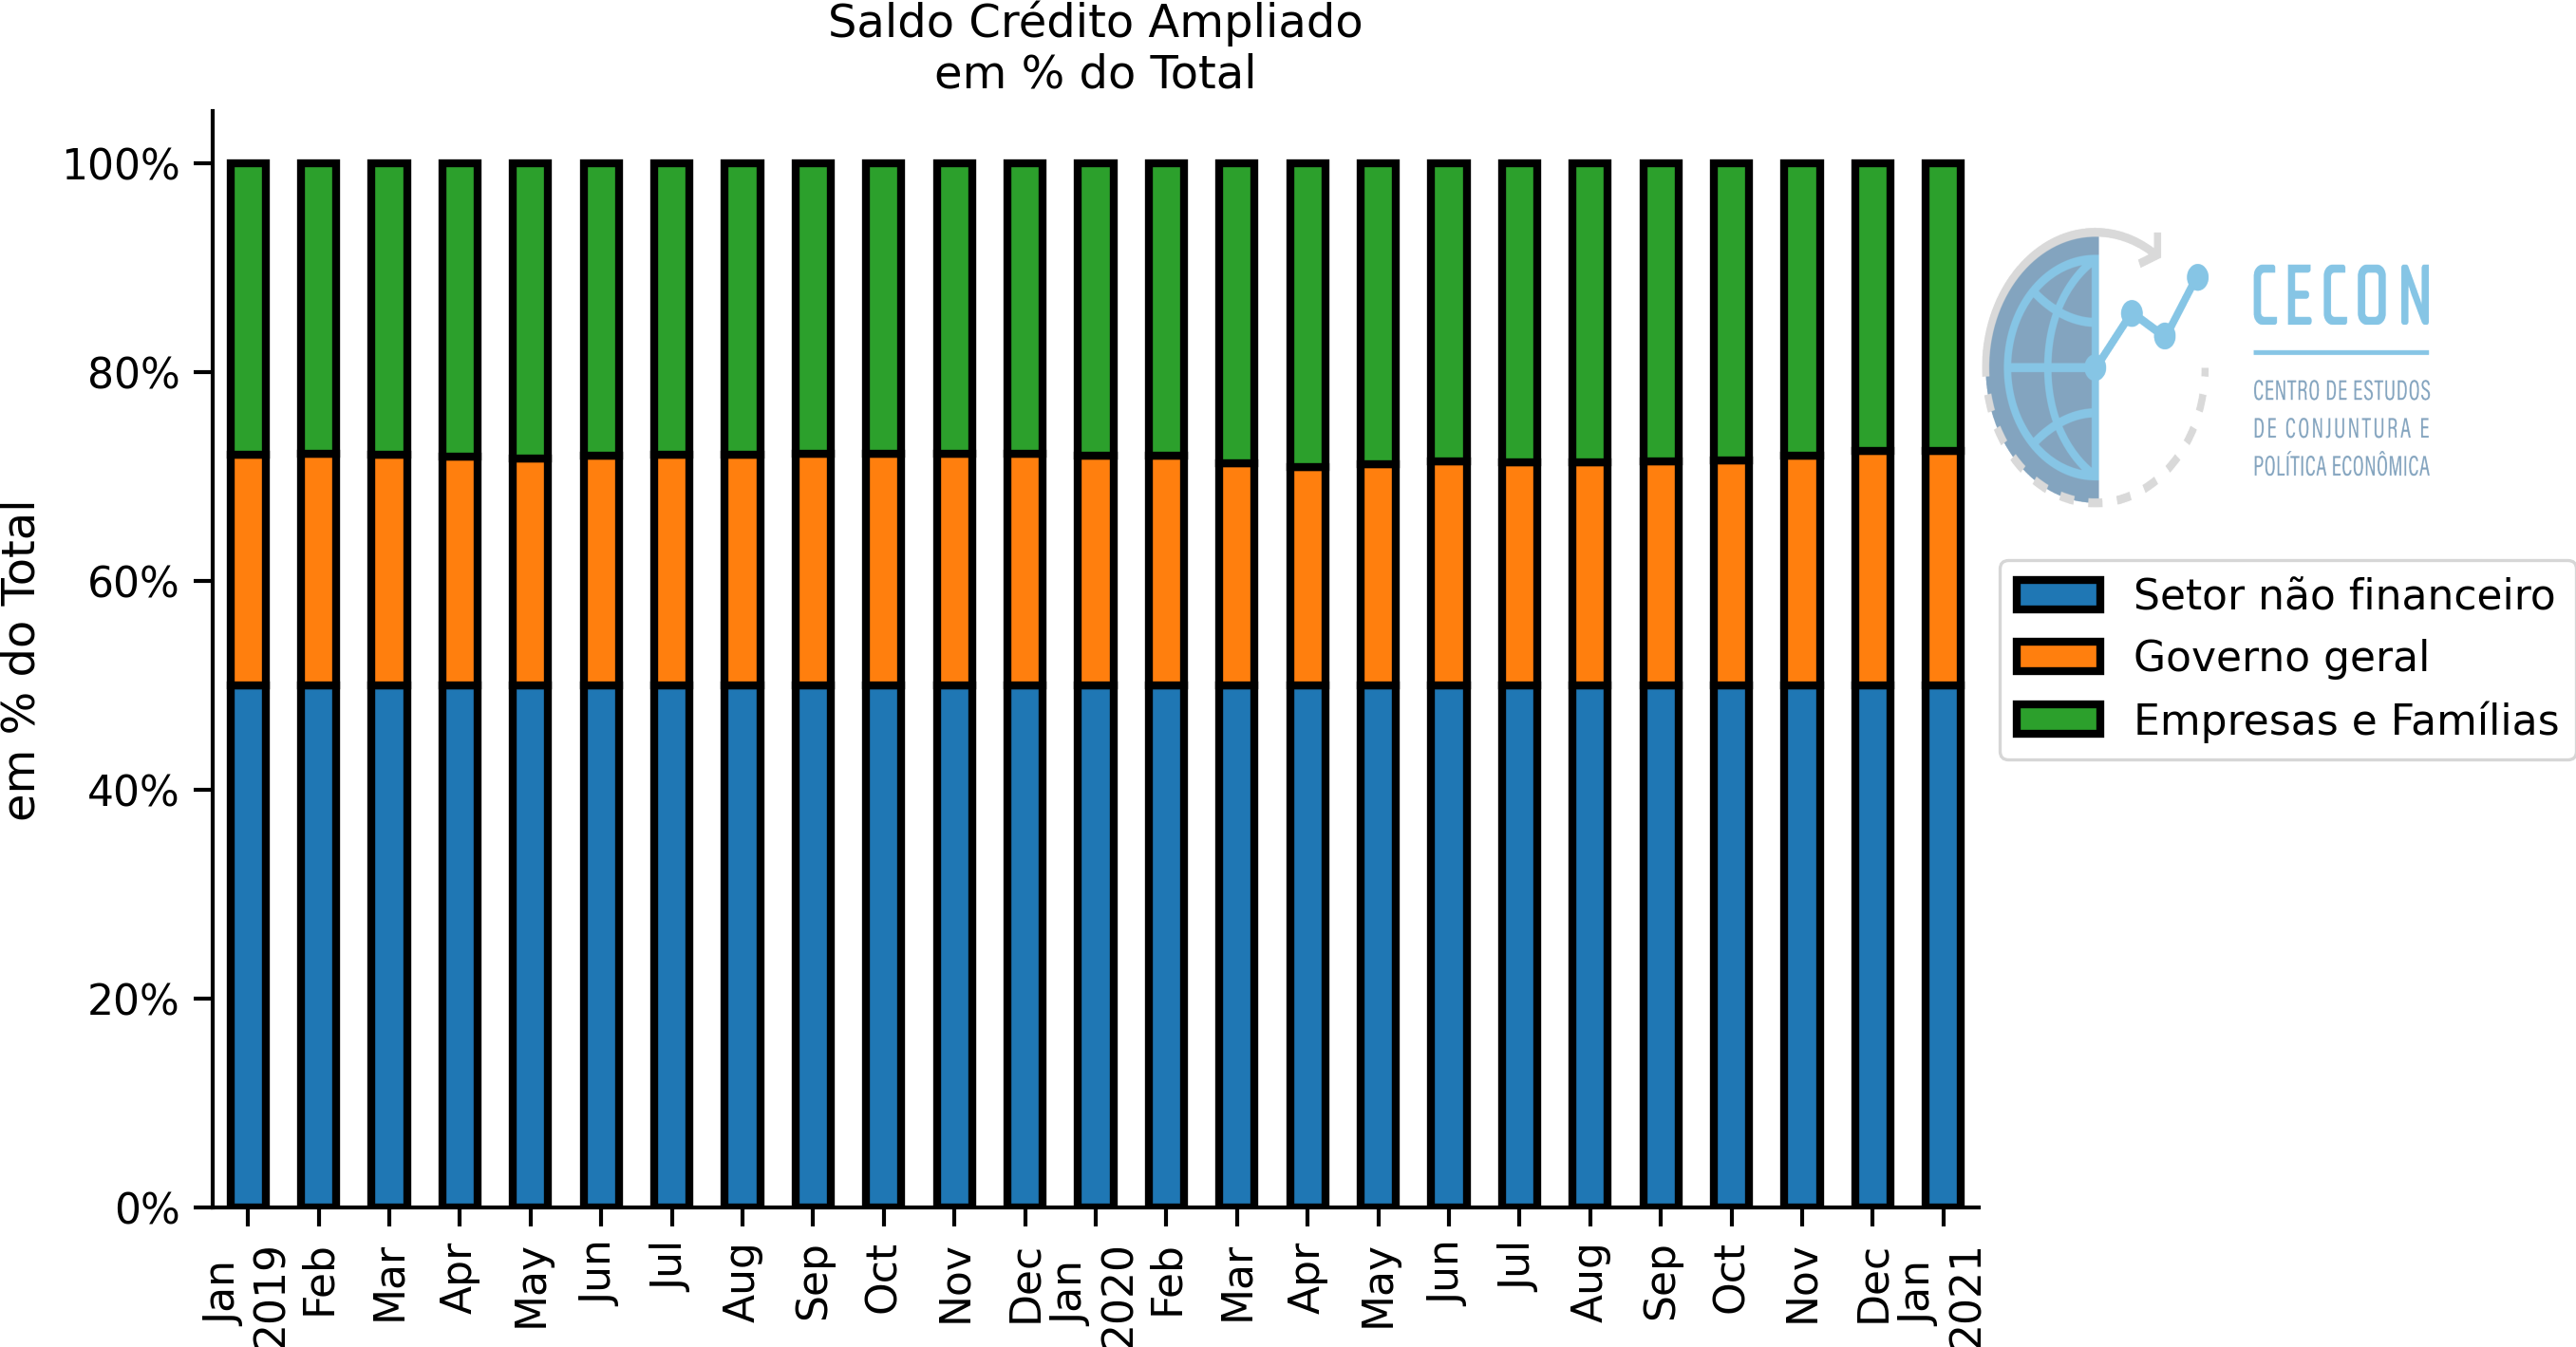
\includegraphics[width=.9\linewidth]{./figs/Credito/SaldoCreditoAmpliado_Total.png}
\end{center}

\subsection*{Indicadores de aprovação de crédito}
\label{sec:org4b05186}

\begin{center}
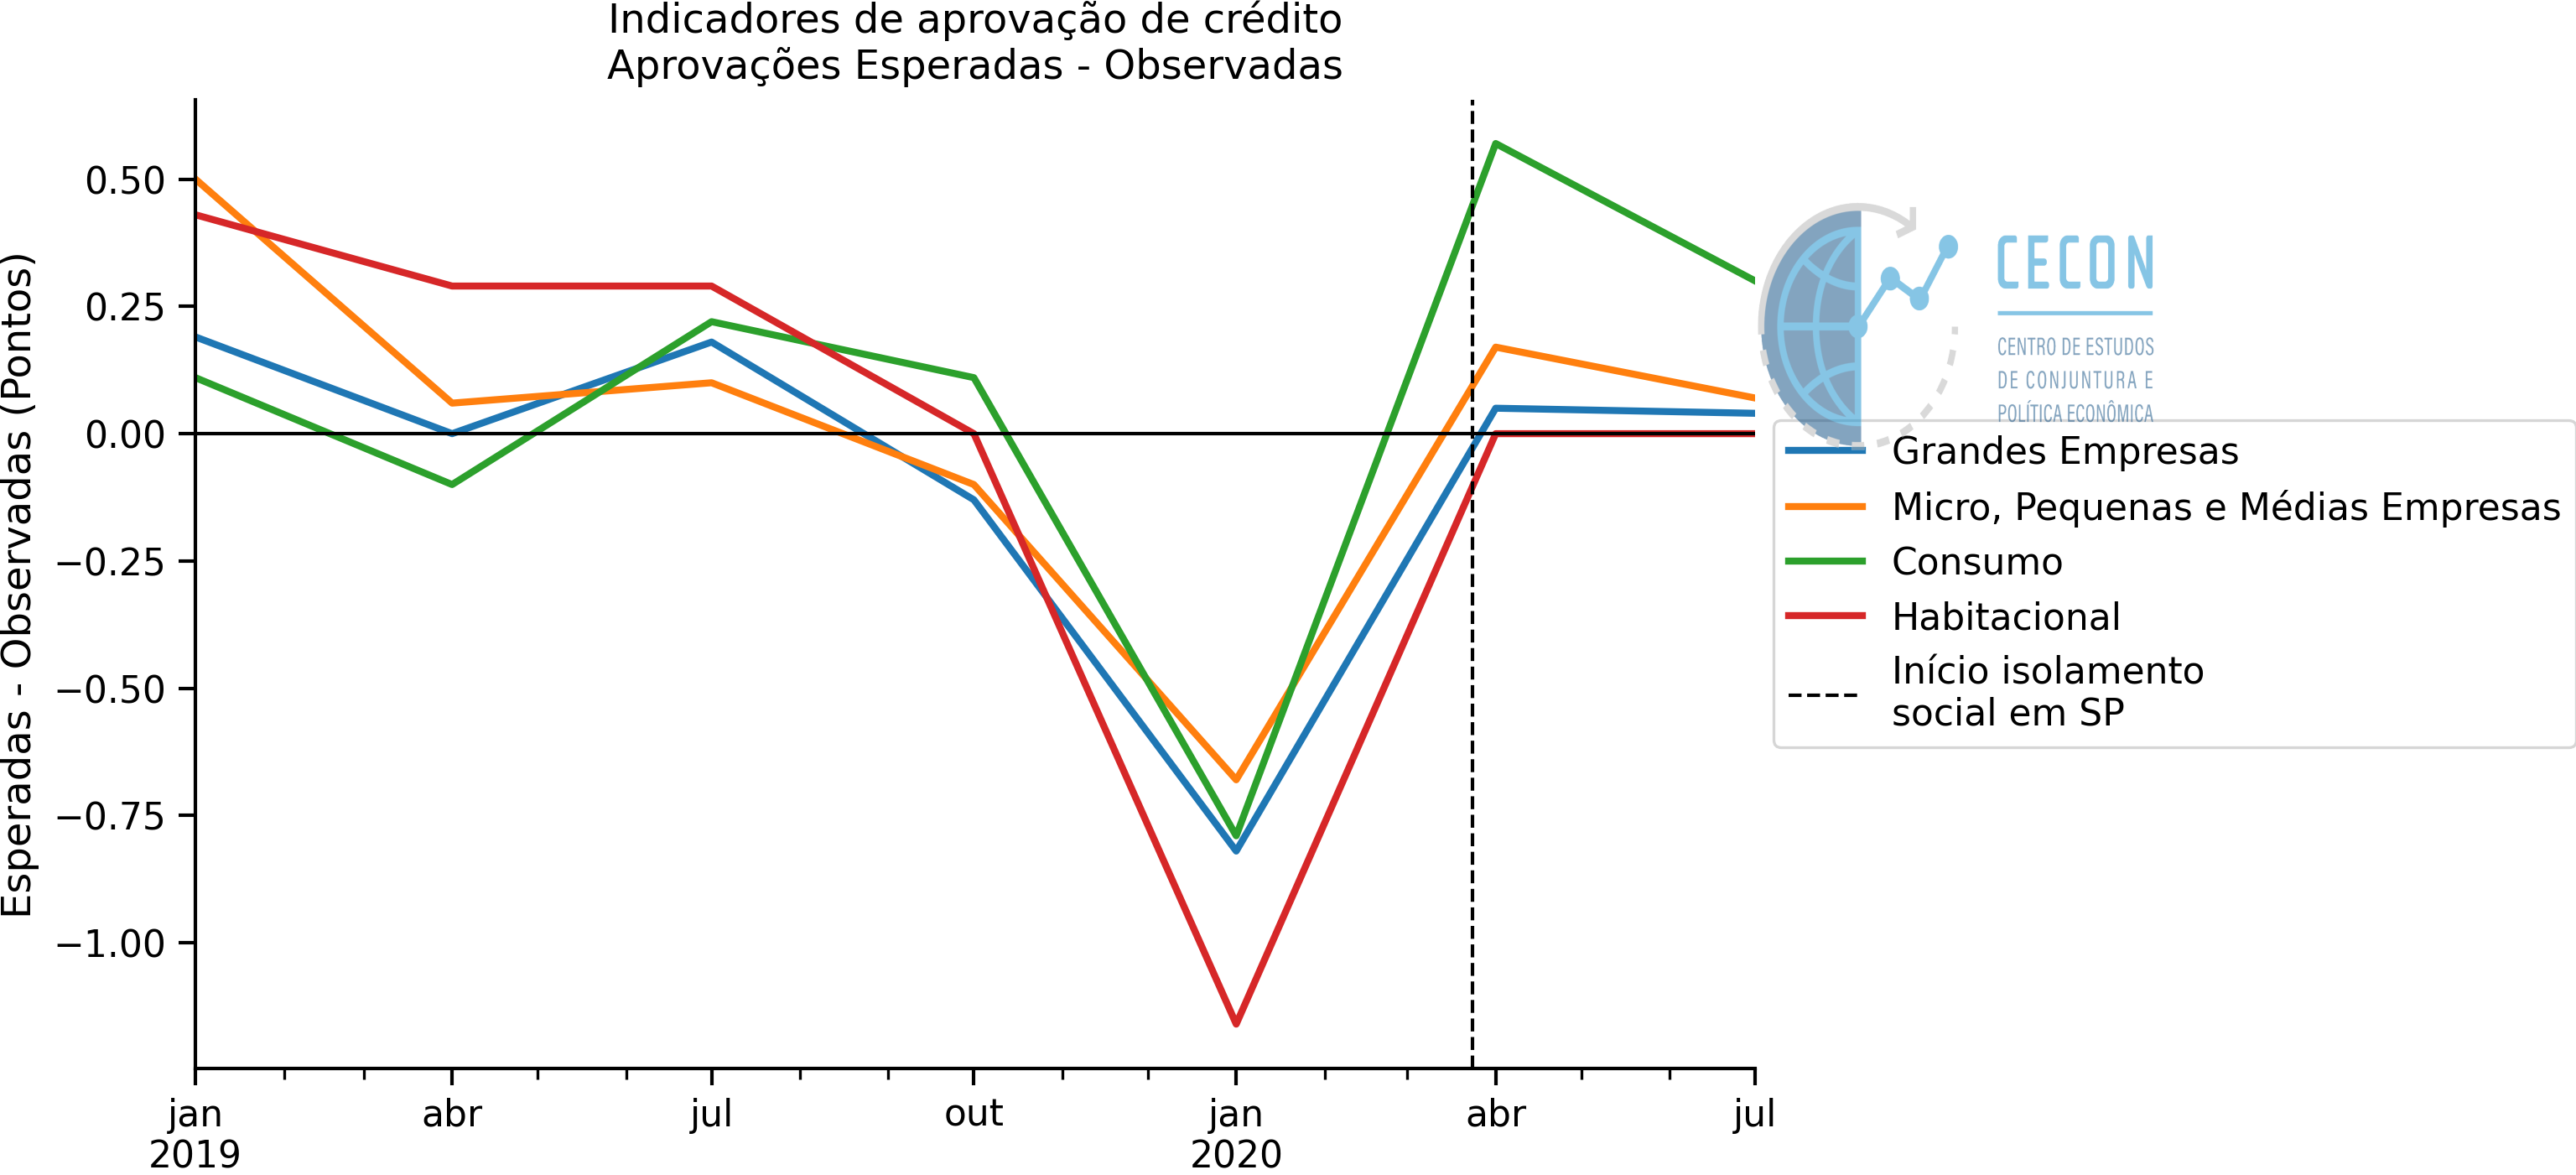
\includegraphics[width=.9\linewidth]{./figs/Credito/PTC.png}
\end{center}

\subsection*{Recolhimentos compulsórios de instituições financeiras}
\label{sec:org8ce43c9}

\begin{center}
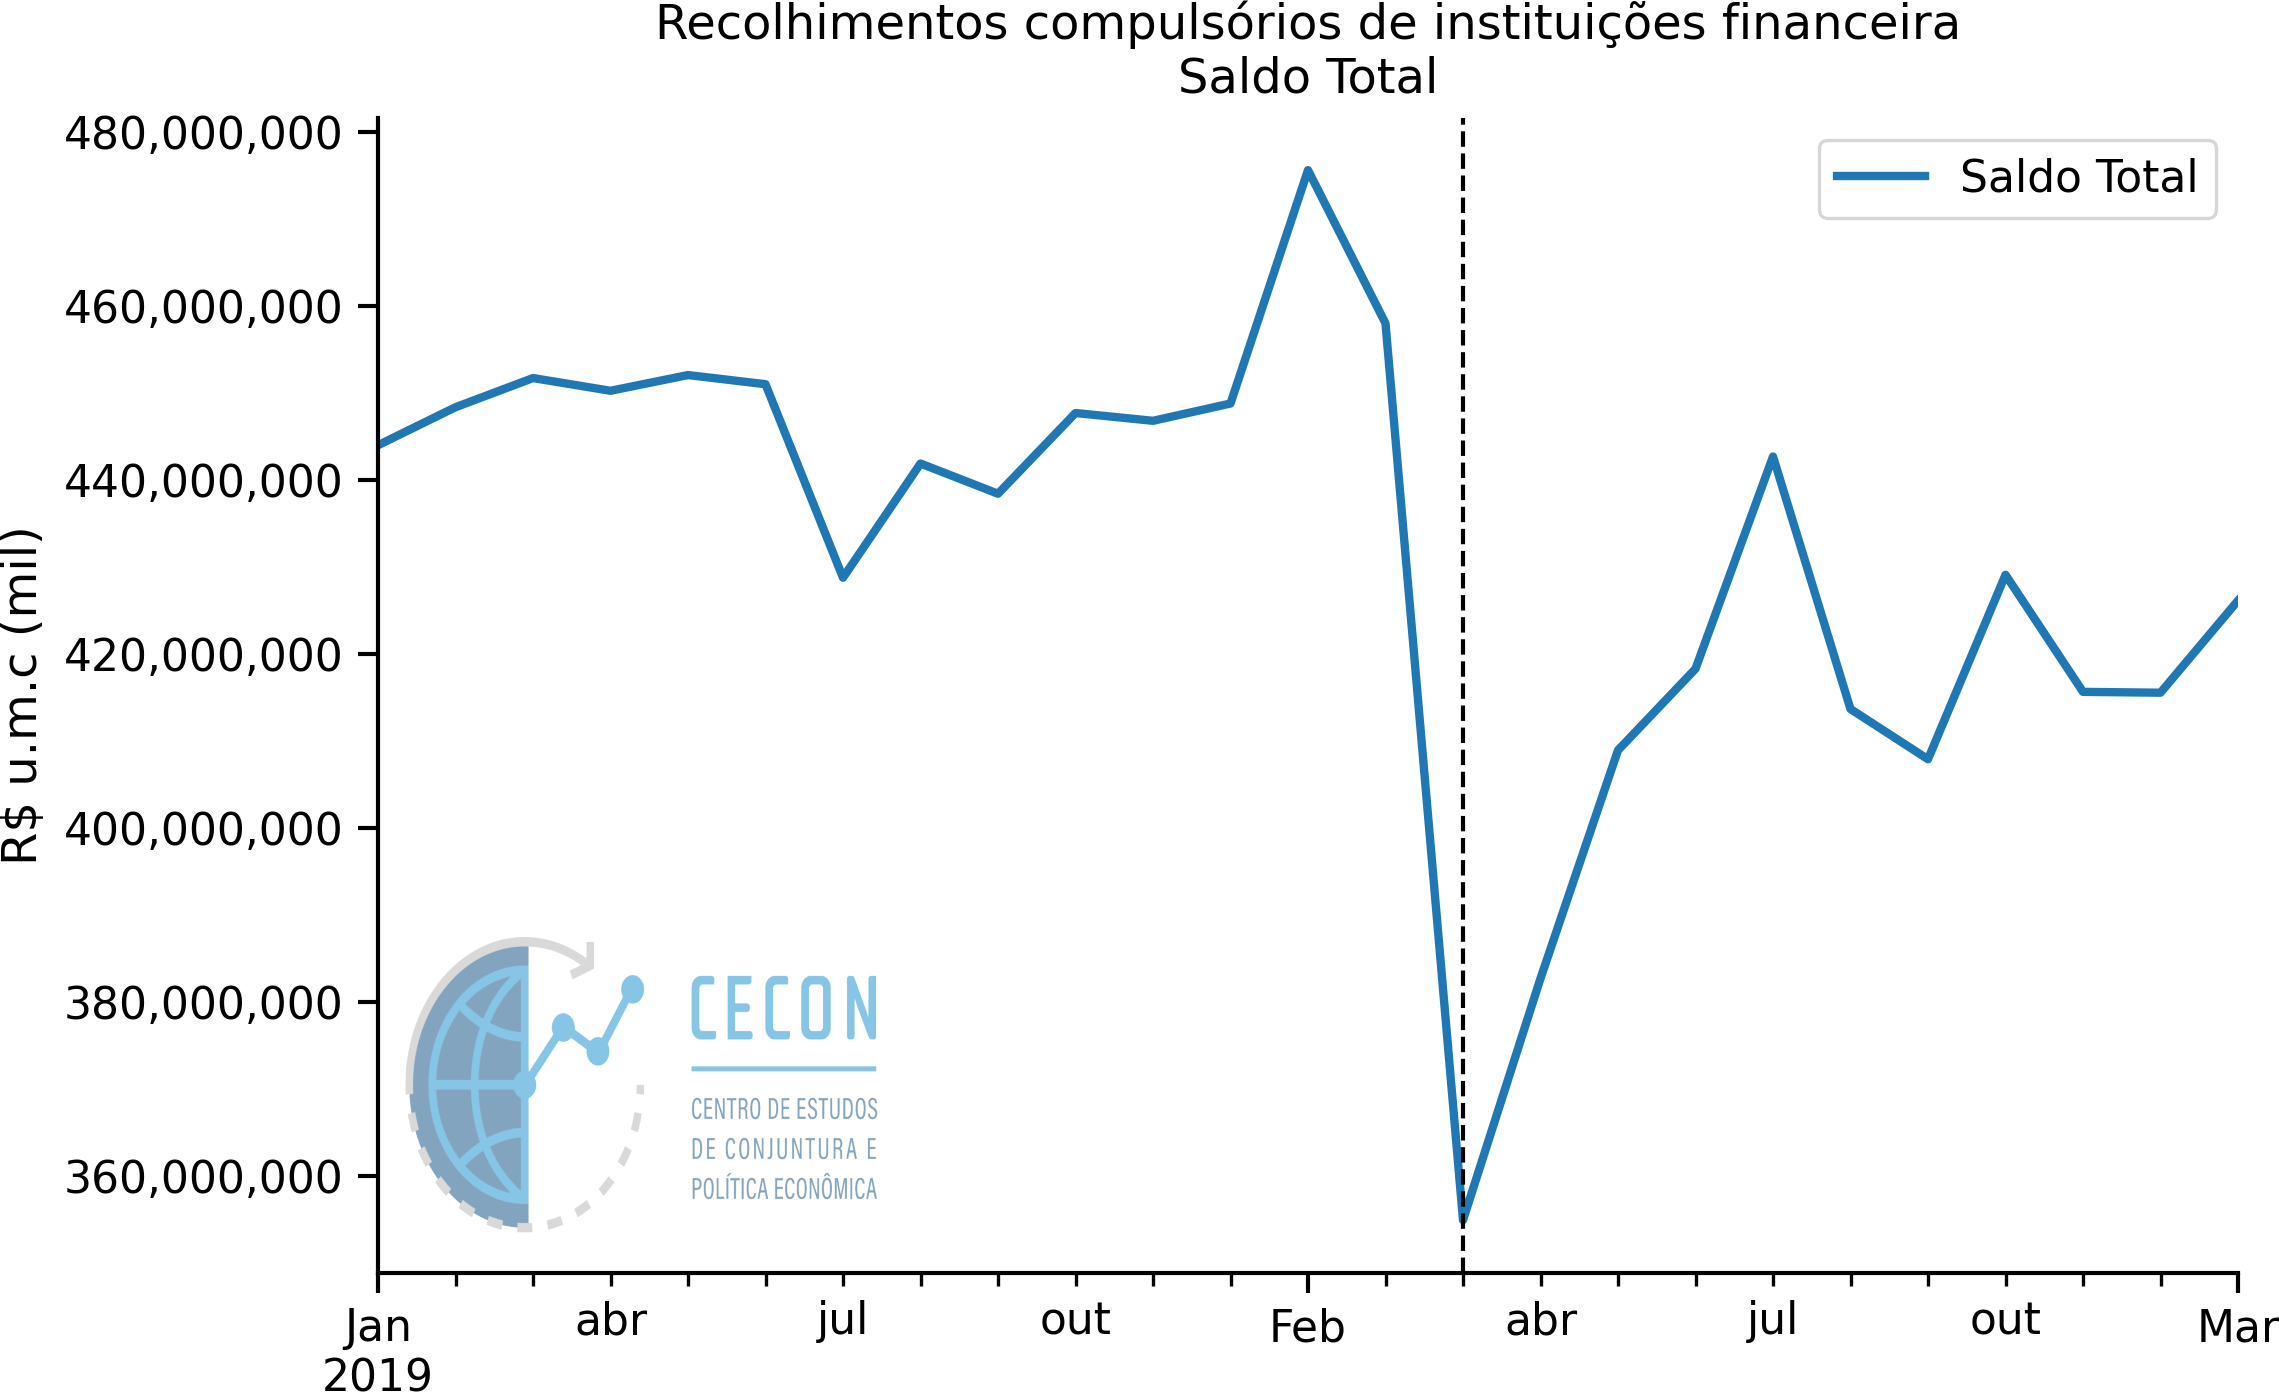
\includegraphics[width=.9\linewidth]{./figs/Credito/Recolhimentos_Total.png}
\end{center}

\section*{Índices de atividade setoriais}
\label{sec:org543ce81}


\subsection*{Pesquisa Mensal do Comércio (PMC)}
\label{sec:org8af1d09}

\begin{center}
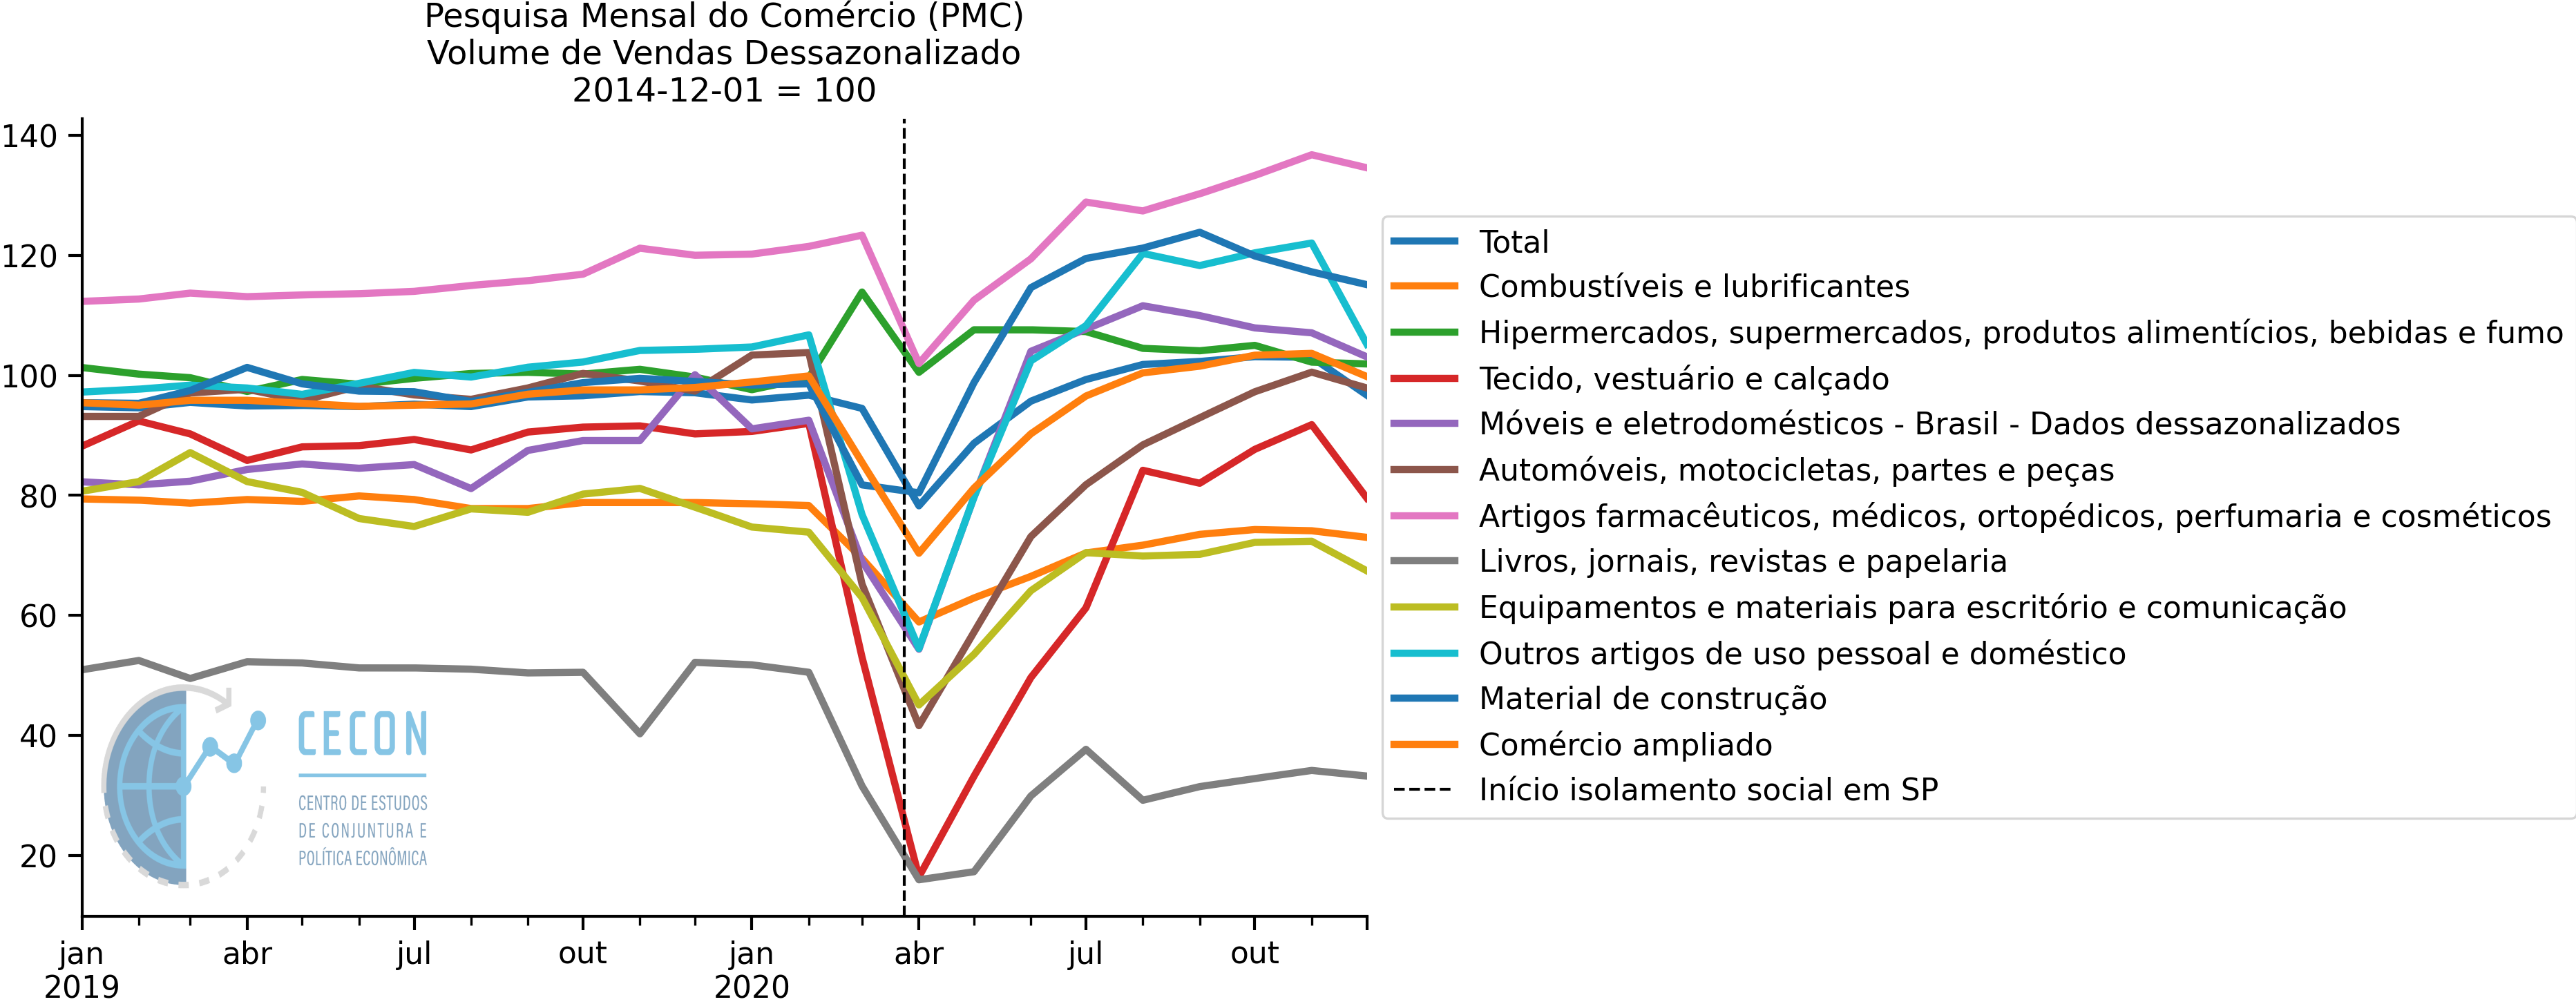
\includegraphics[width=.9\linewidth]{./figs/Setoriais/PMC_IBGE.png}
\end{center}


\subsection*{Pesquisa Industrial Mensal (PIM)}
\label{sec:org16c12f8}

\begin{center}
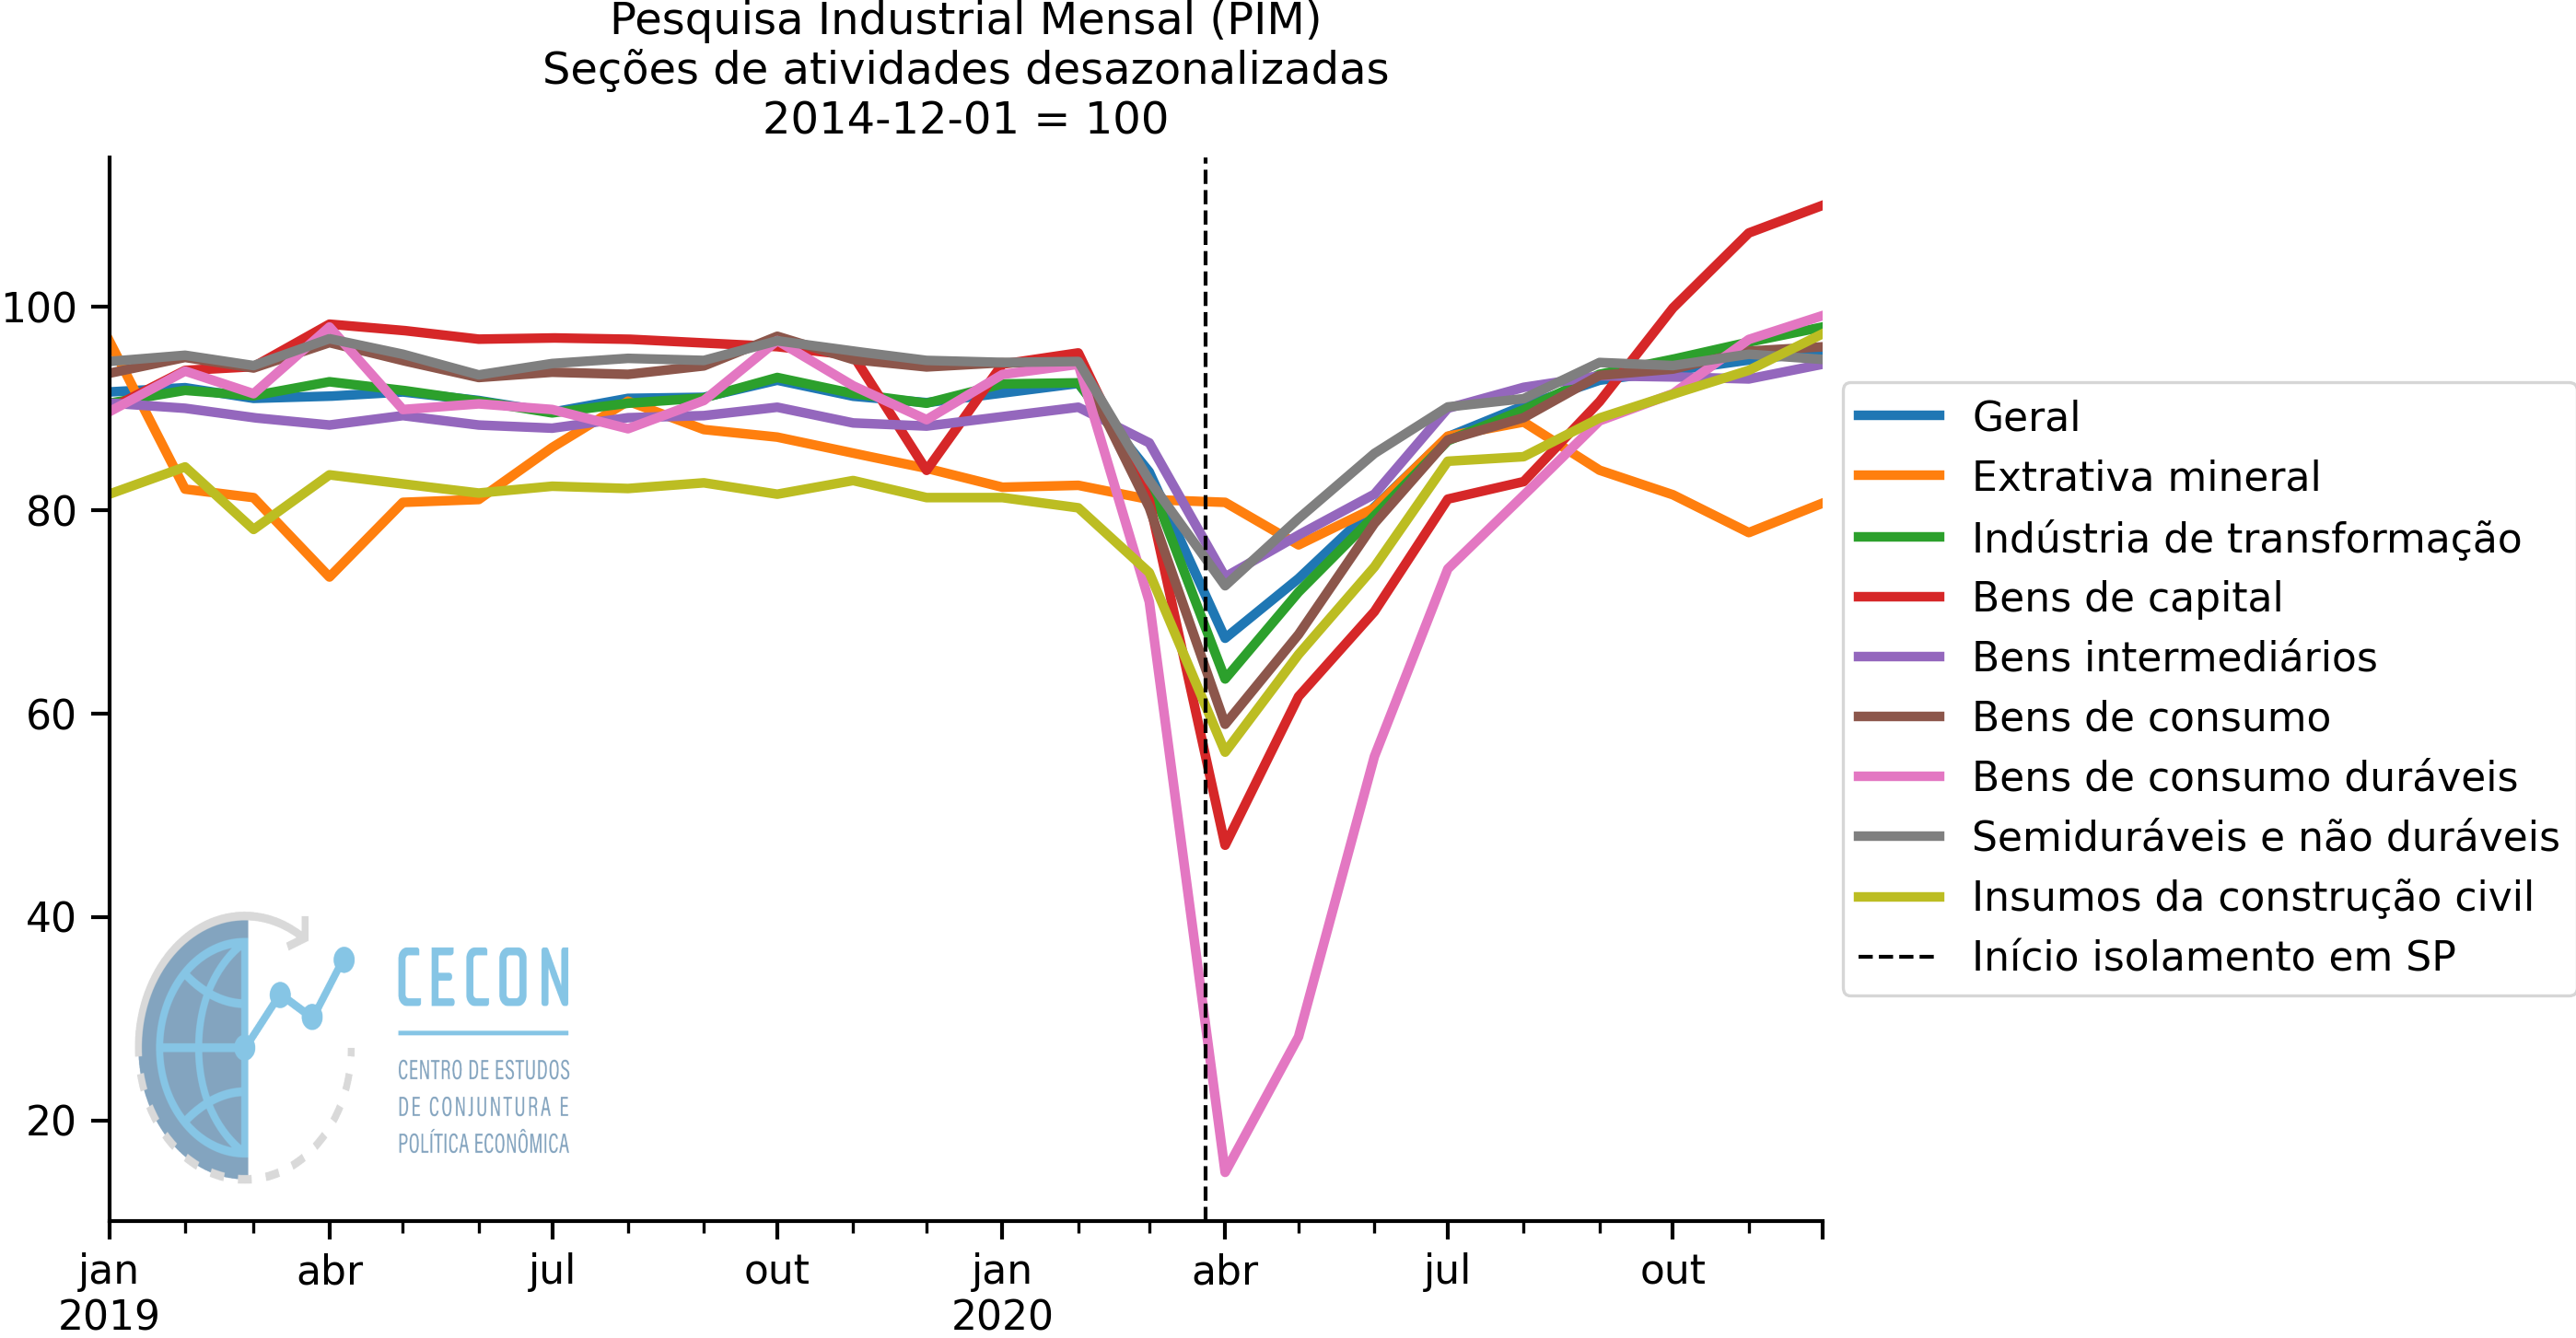
\includegraphics[width=.9\linewidth]{./figs/Setoriais/PIM_IBGE.png}
\end{center}


\subsection*{Pesquisa Mensal de Serviços (PMS)}
\label{sec:org2edeccc}

\section*{Emprego}
\label{sec:org67cbbb3}

\subsection*{Rendimento médio real habitual das pessoas ocupadas}
\label{sec:orgad42c86}


\begin{center}
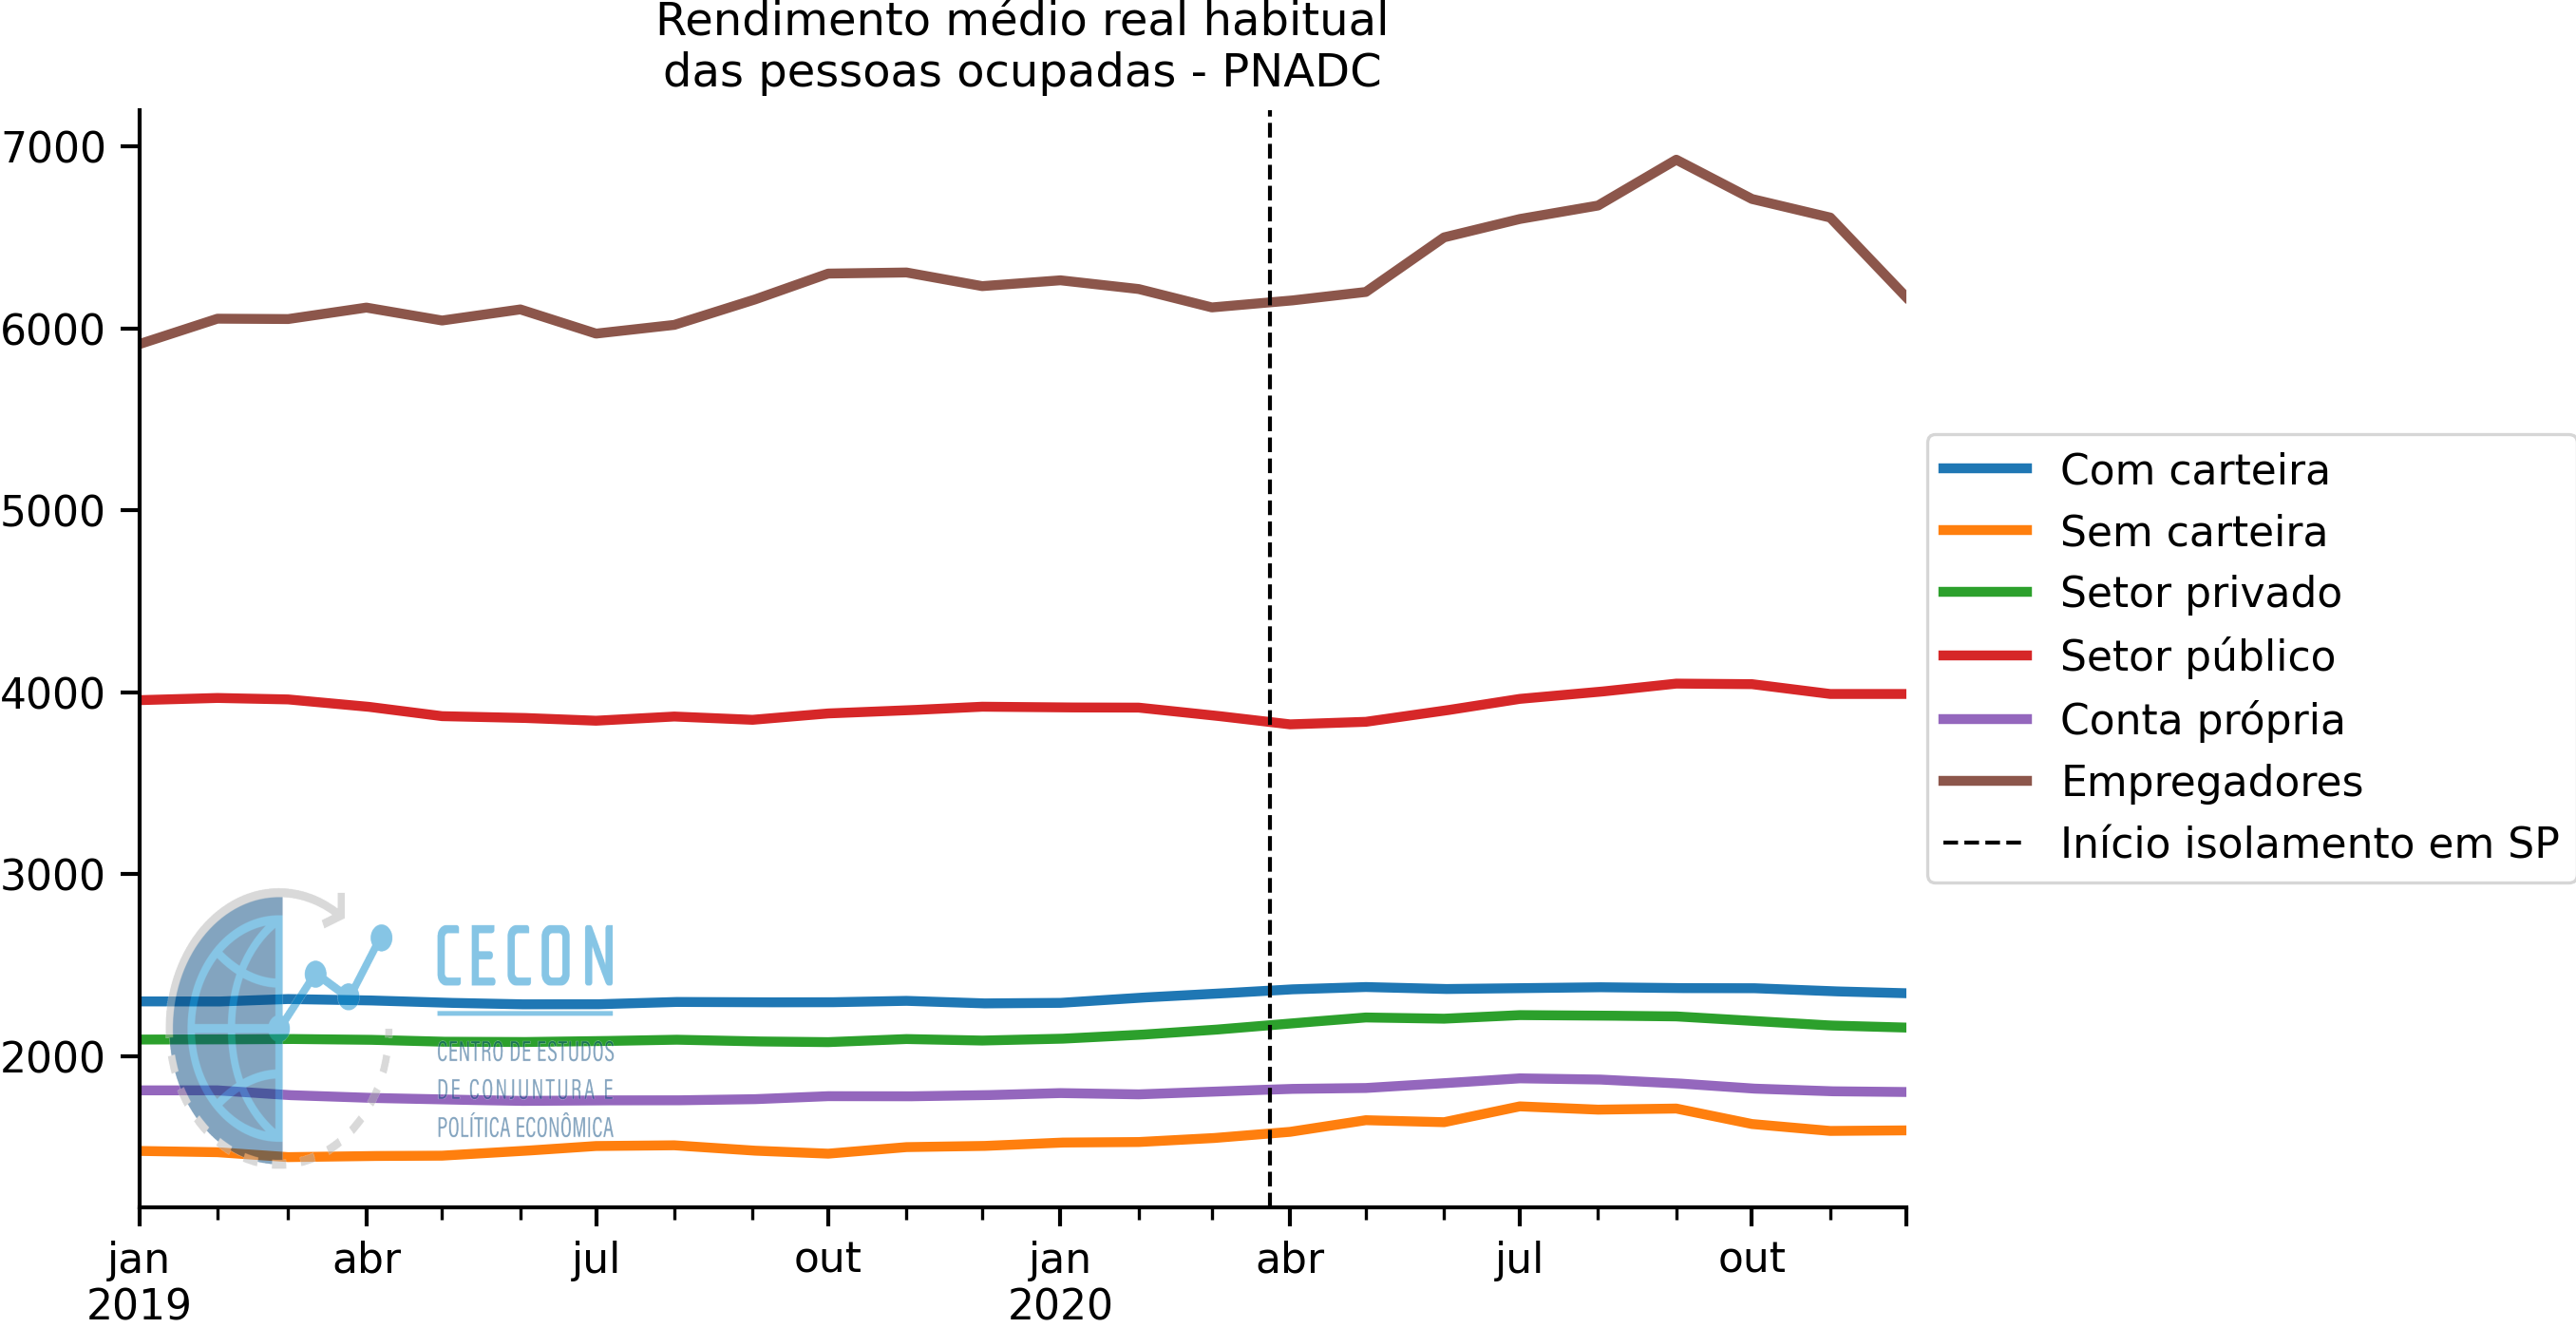
\includegraphics[width=.9\linewidth]{./figs/Emprego/RMHPO.png}
\end{center}

\subsection*{Massa de rendimento real efetiva e habitual de todos os trabalhos}
\label{sec:org04ecf99}

\begin{center}
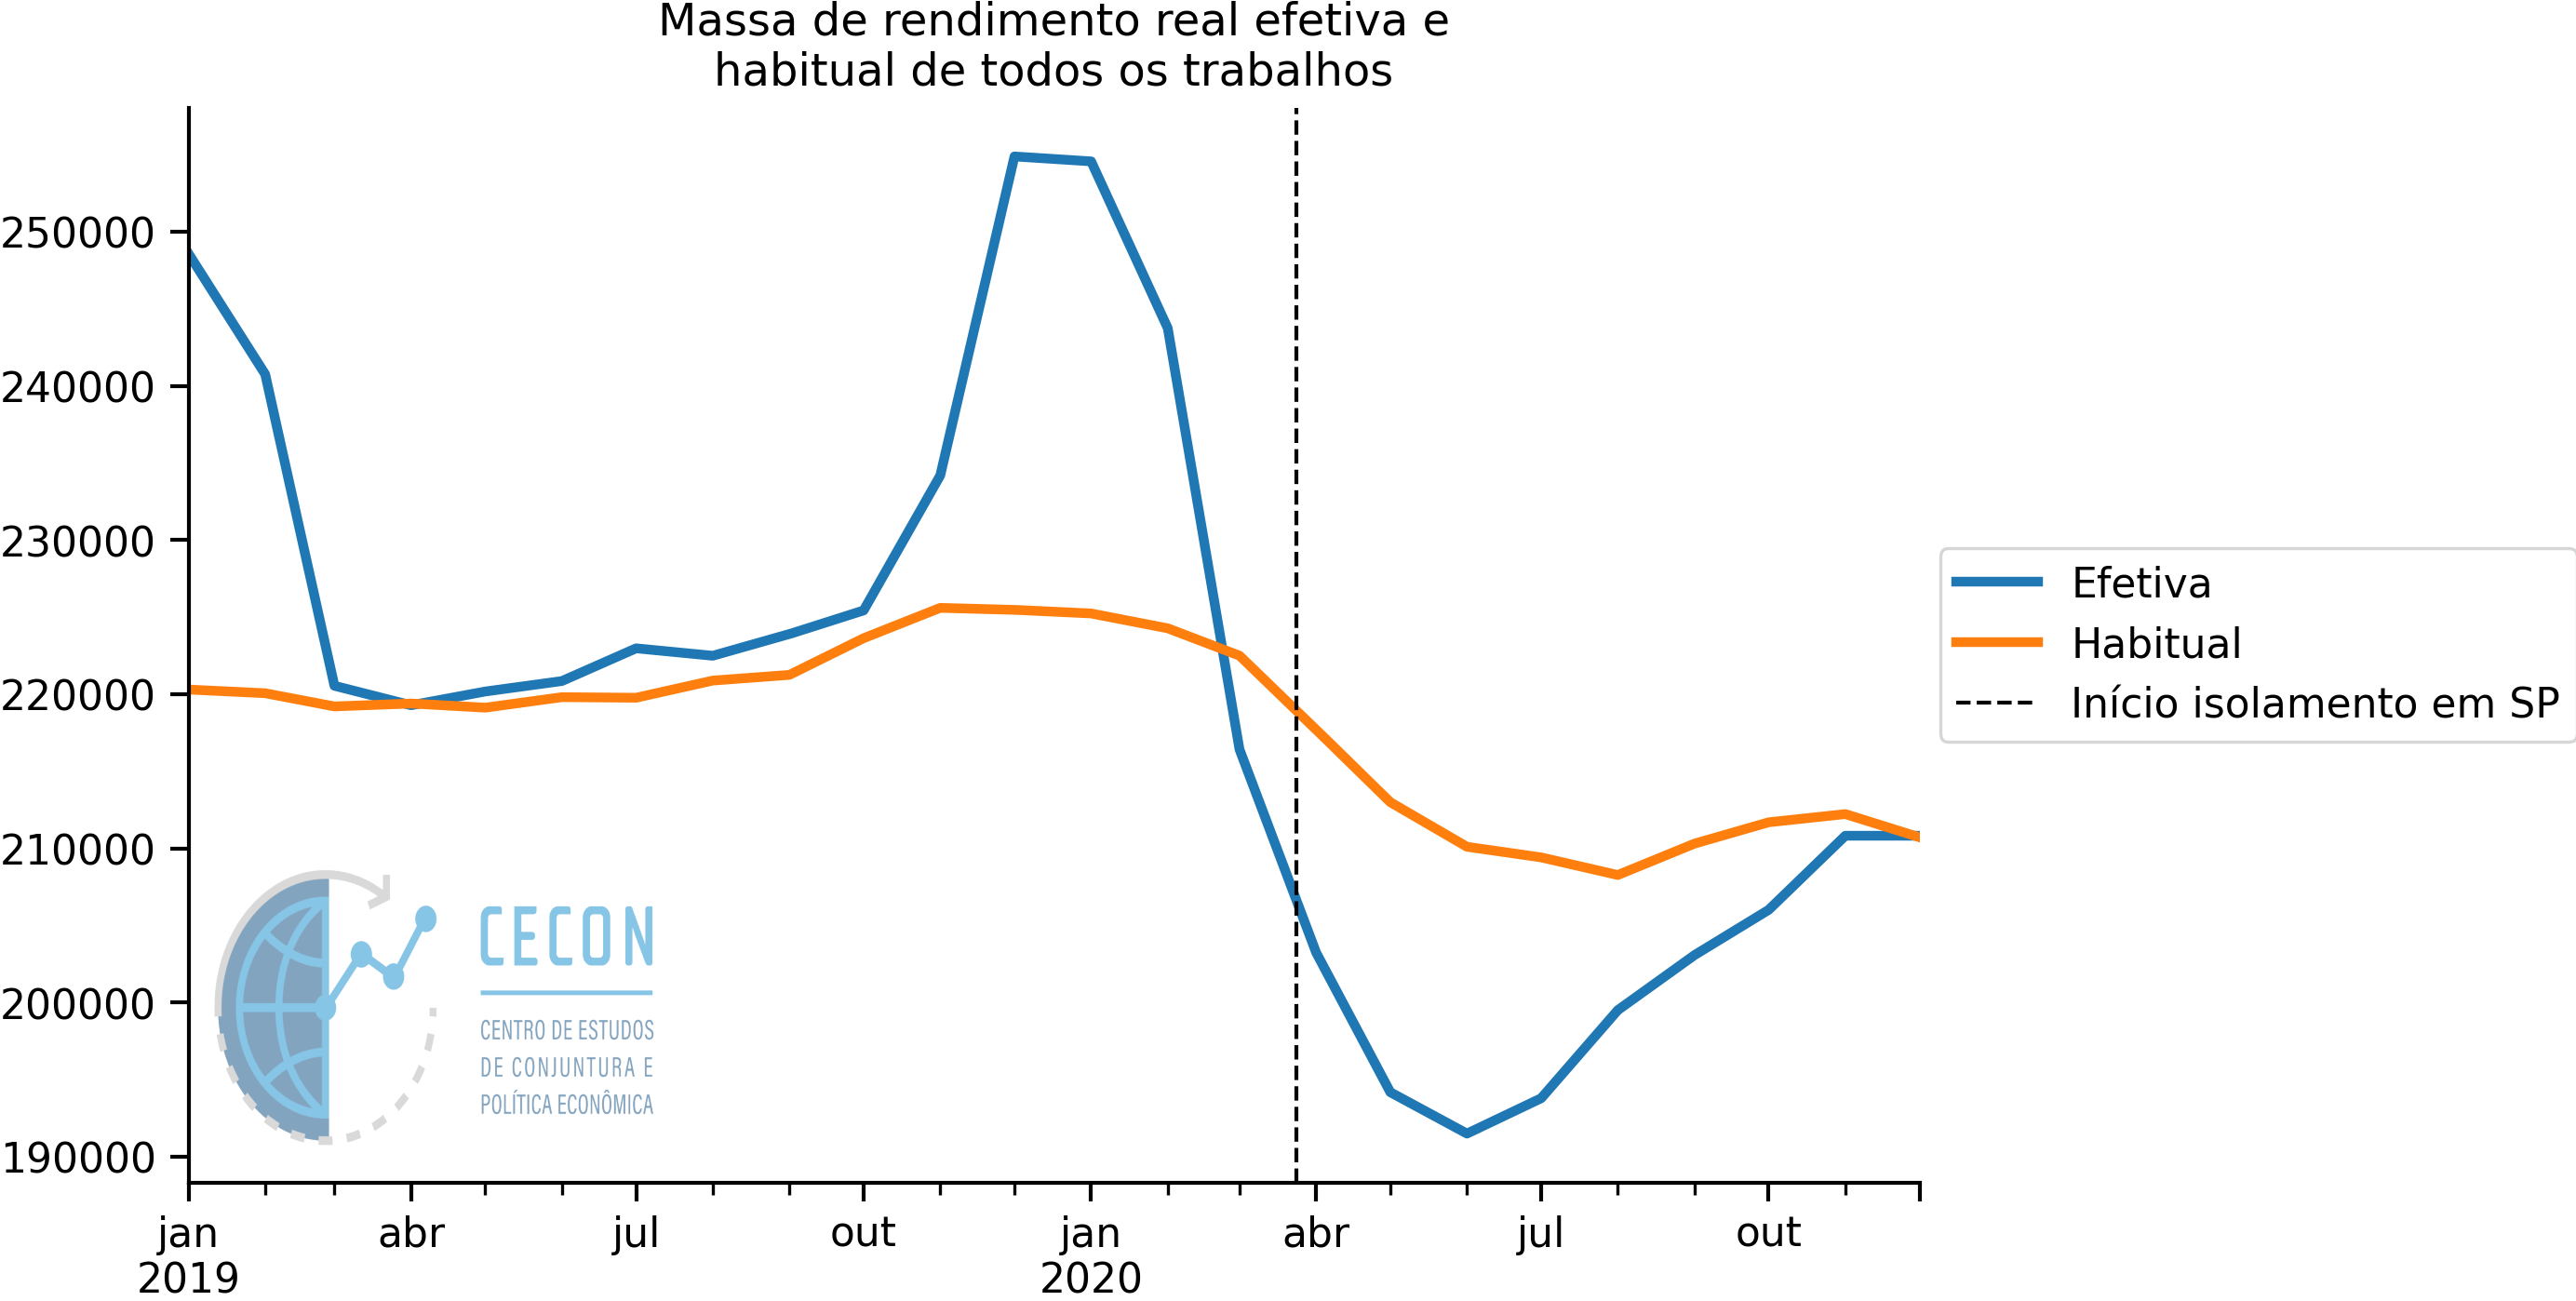
\includegraphics[width=.9\linewidth]{./figs/Emprego/MRR_Efetiva_Habitual.png}
\end{center}

\subsection*{Massa Salarial Ampliada Disponível - PNADC}
\label{sec:orgf790e83}

\begin{center}
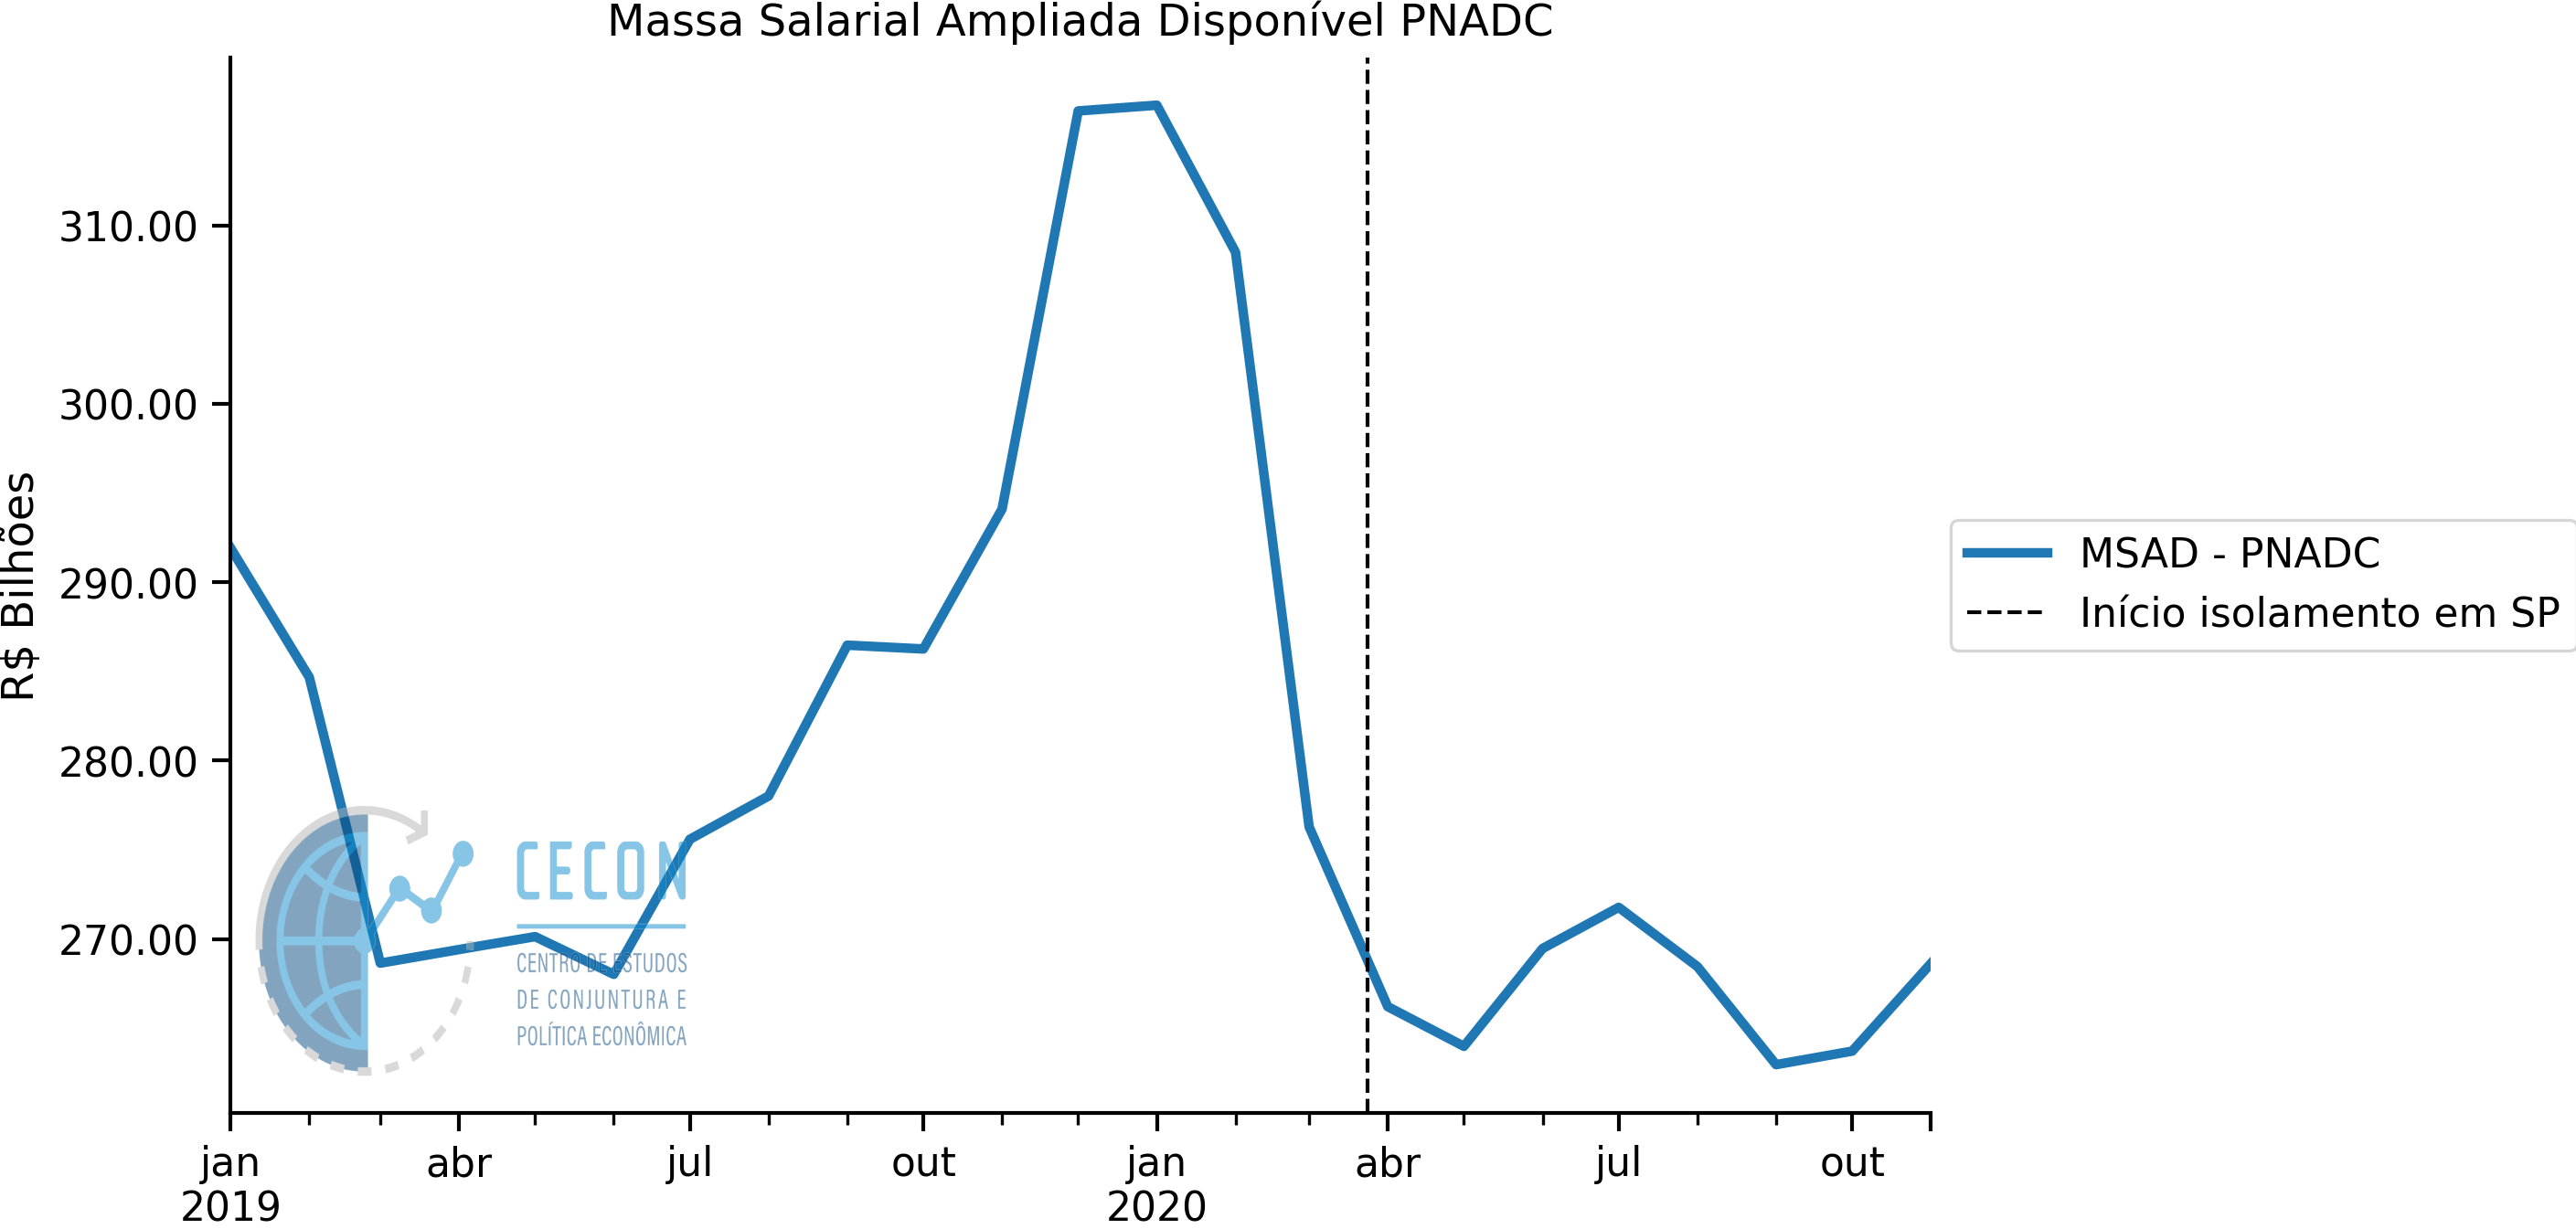
\includegraphics[width=.9\linewidth]{./figs/Emprego/MSAD.png}
\end{center}

\subsection*{Rendimento habitual médio por atividade}
\label{sec:orga69ea6b}

\subsection*{Número de horas trabalhadas - indústria de transformação}
\label{sec:org35f305e}

\begin{center}
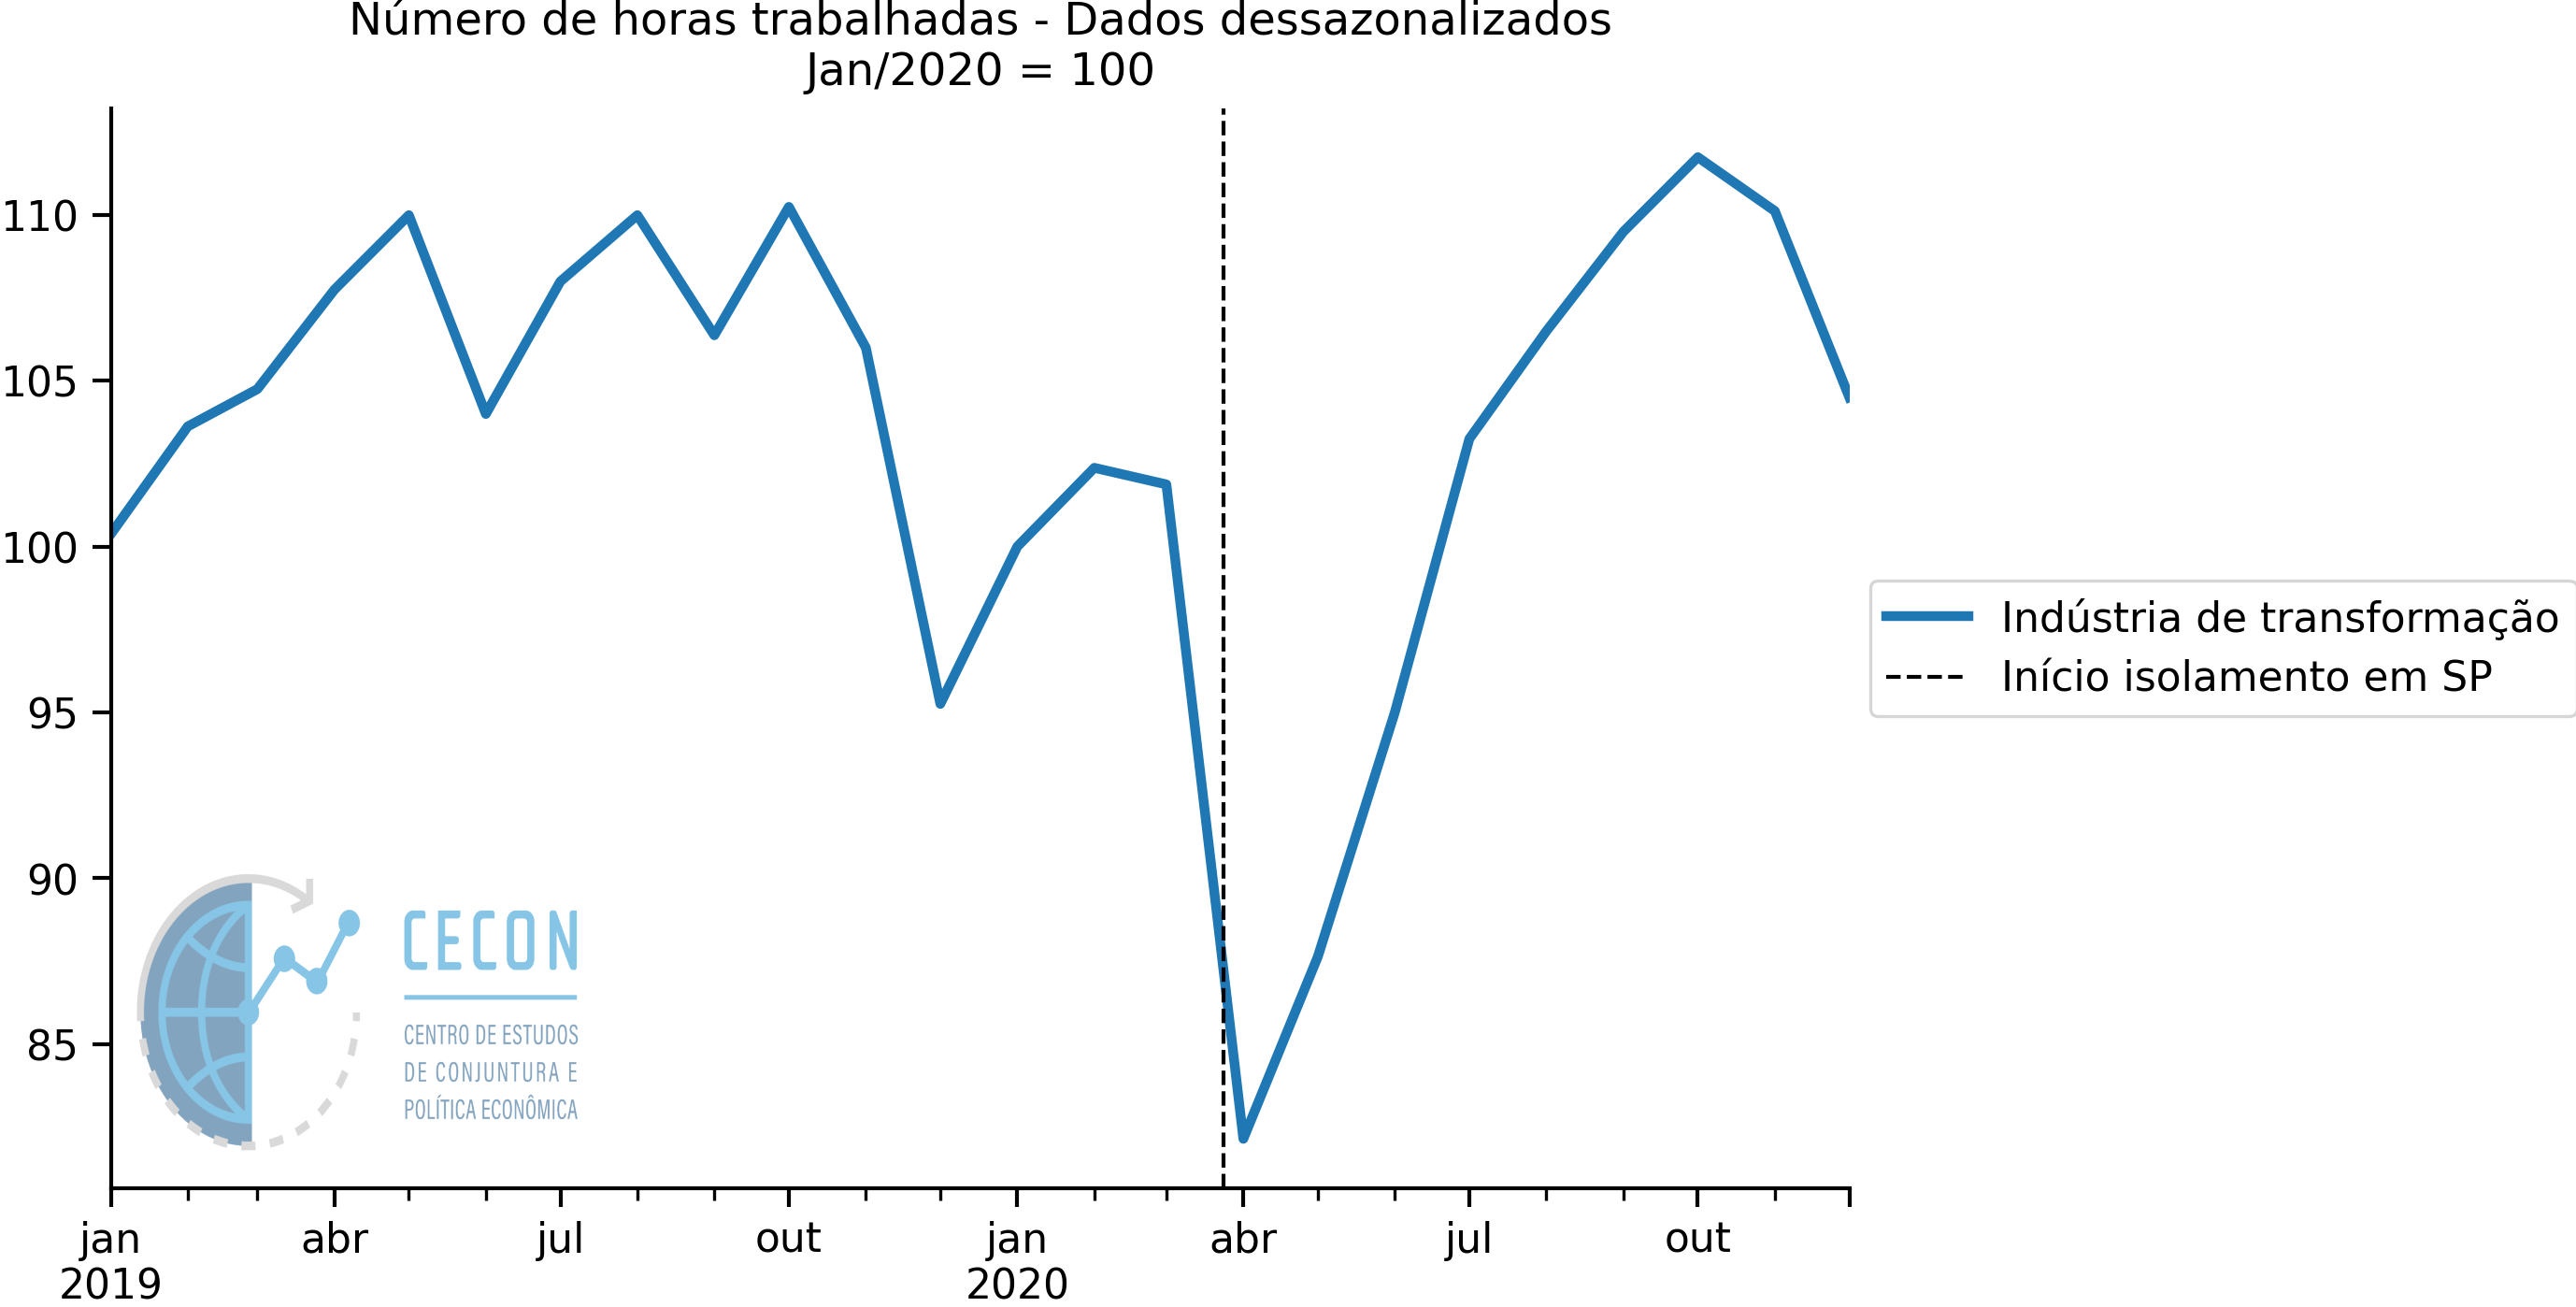
\includegraphics[width=.9\linewidth]{./figs/Emprego/Horas_Transformacao.png}
\end{center}

\subsection*{Novo CAGED  - Por atividade (dados dessazonalizados)}
\label{sec:org4c00f1a}

\begin{center}
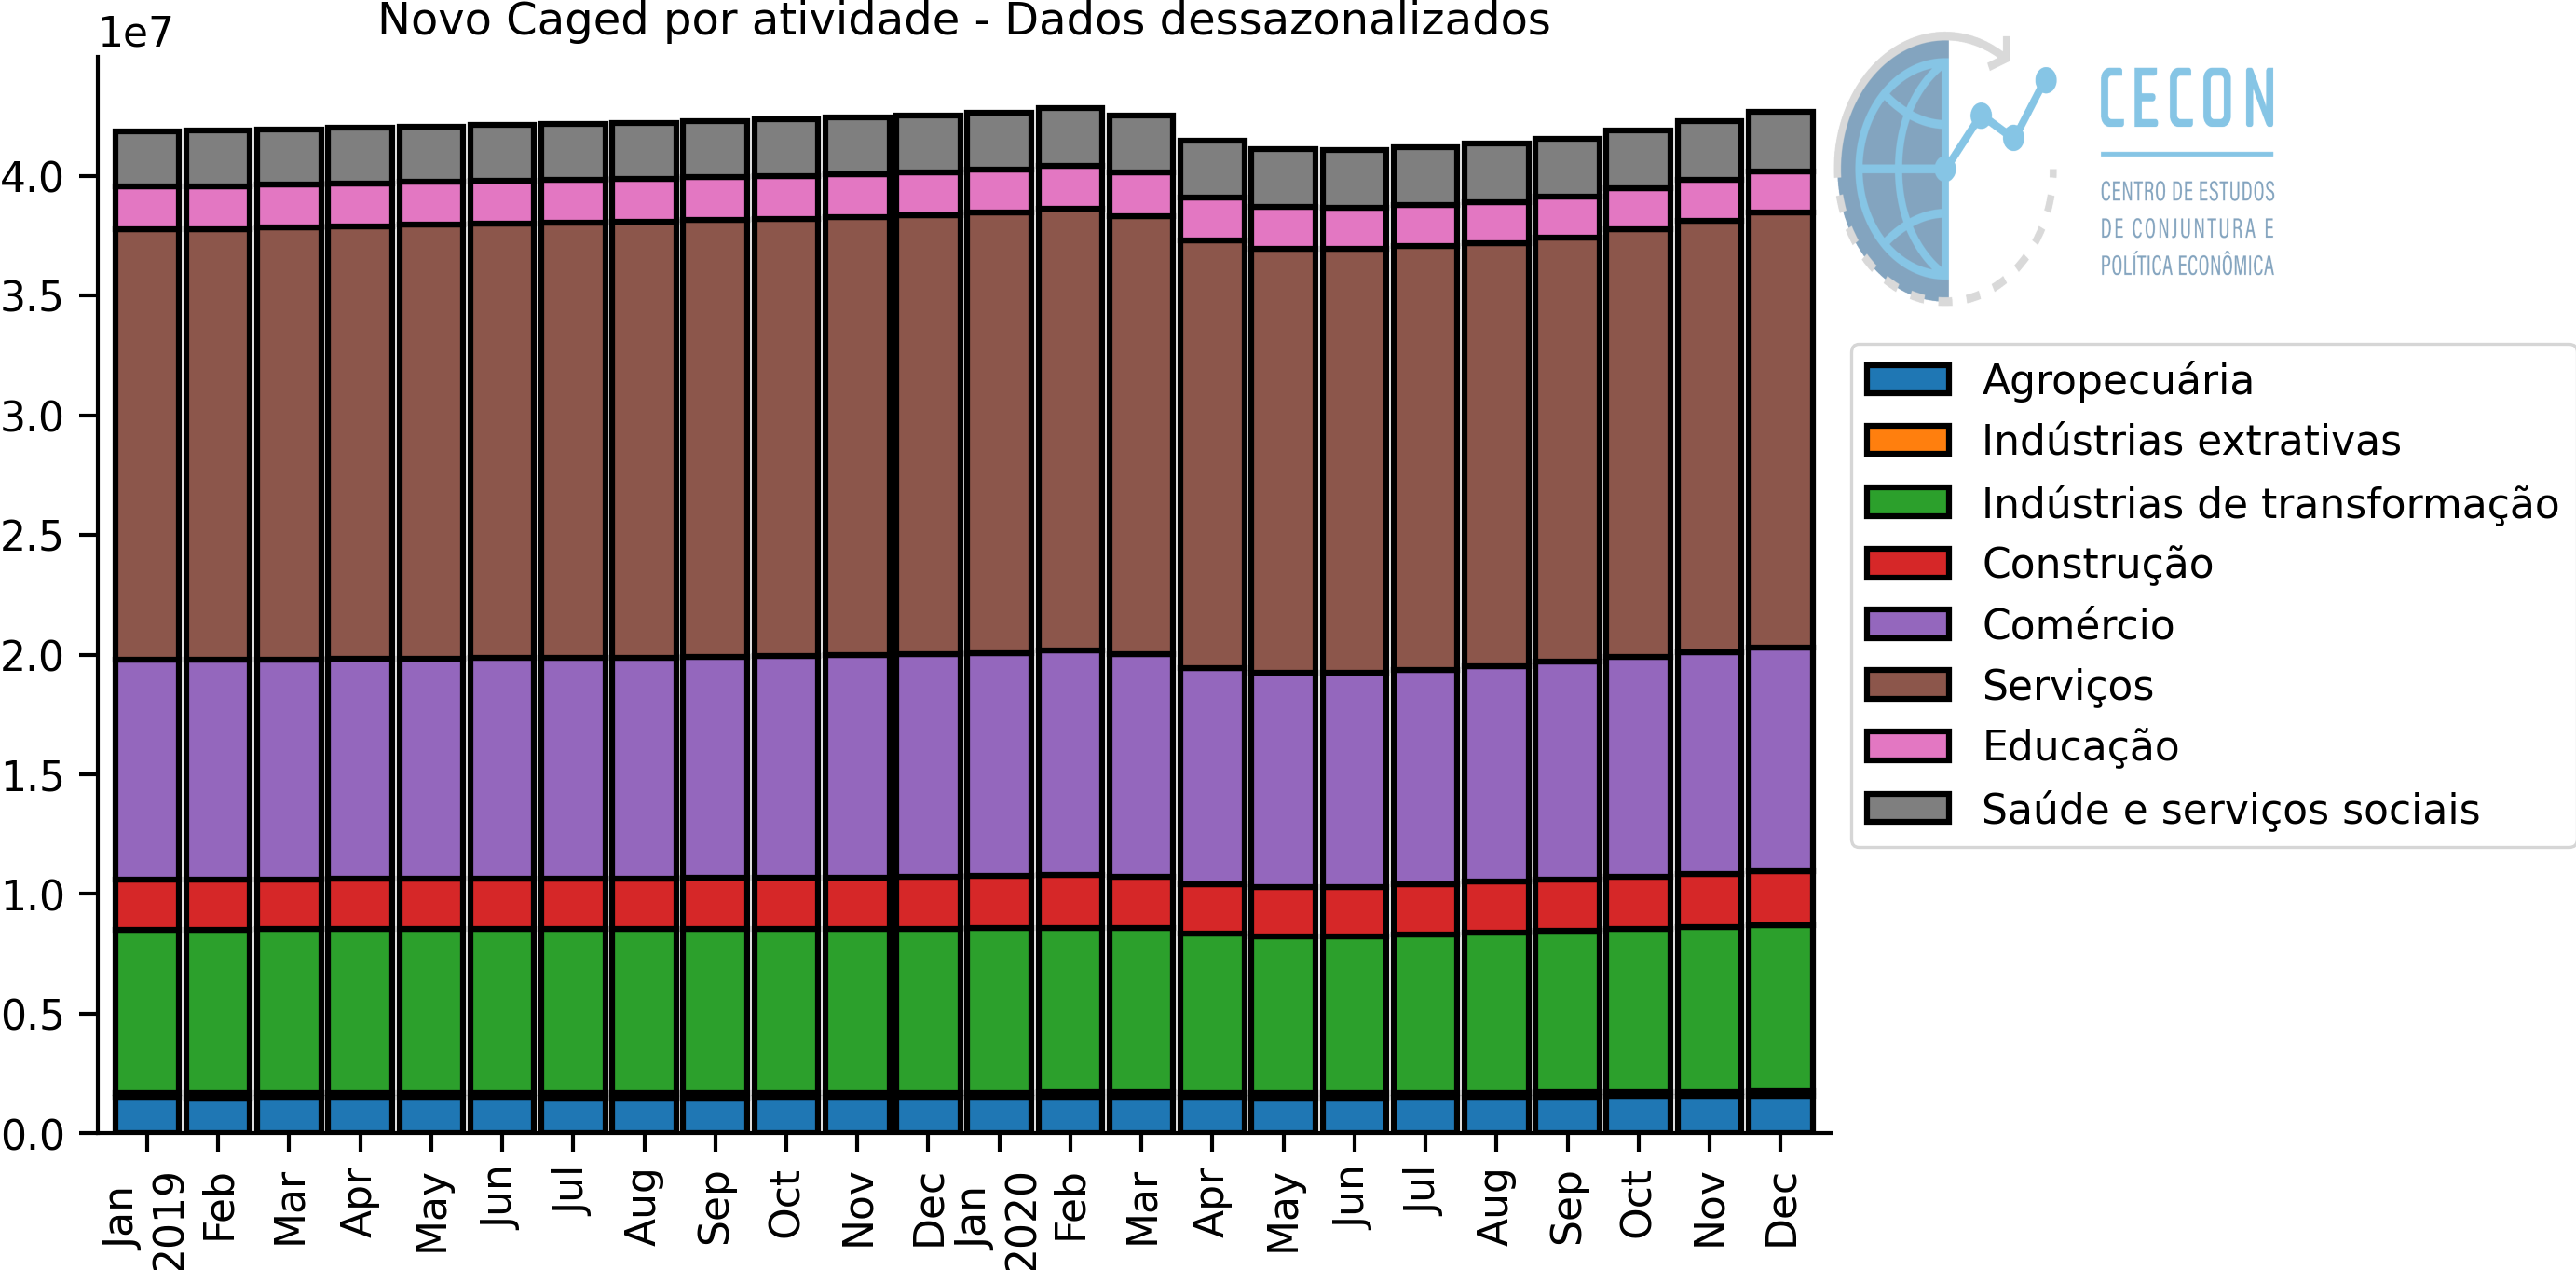
\includegraphics[width=.9\linewidth]{./figs/Emprego/NovoCaged_Atividade.png}
\end{center}



\subsection*{Taxa de desocupação}
\label{sec:org5d0fe1c}

\begin{center}
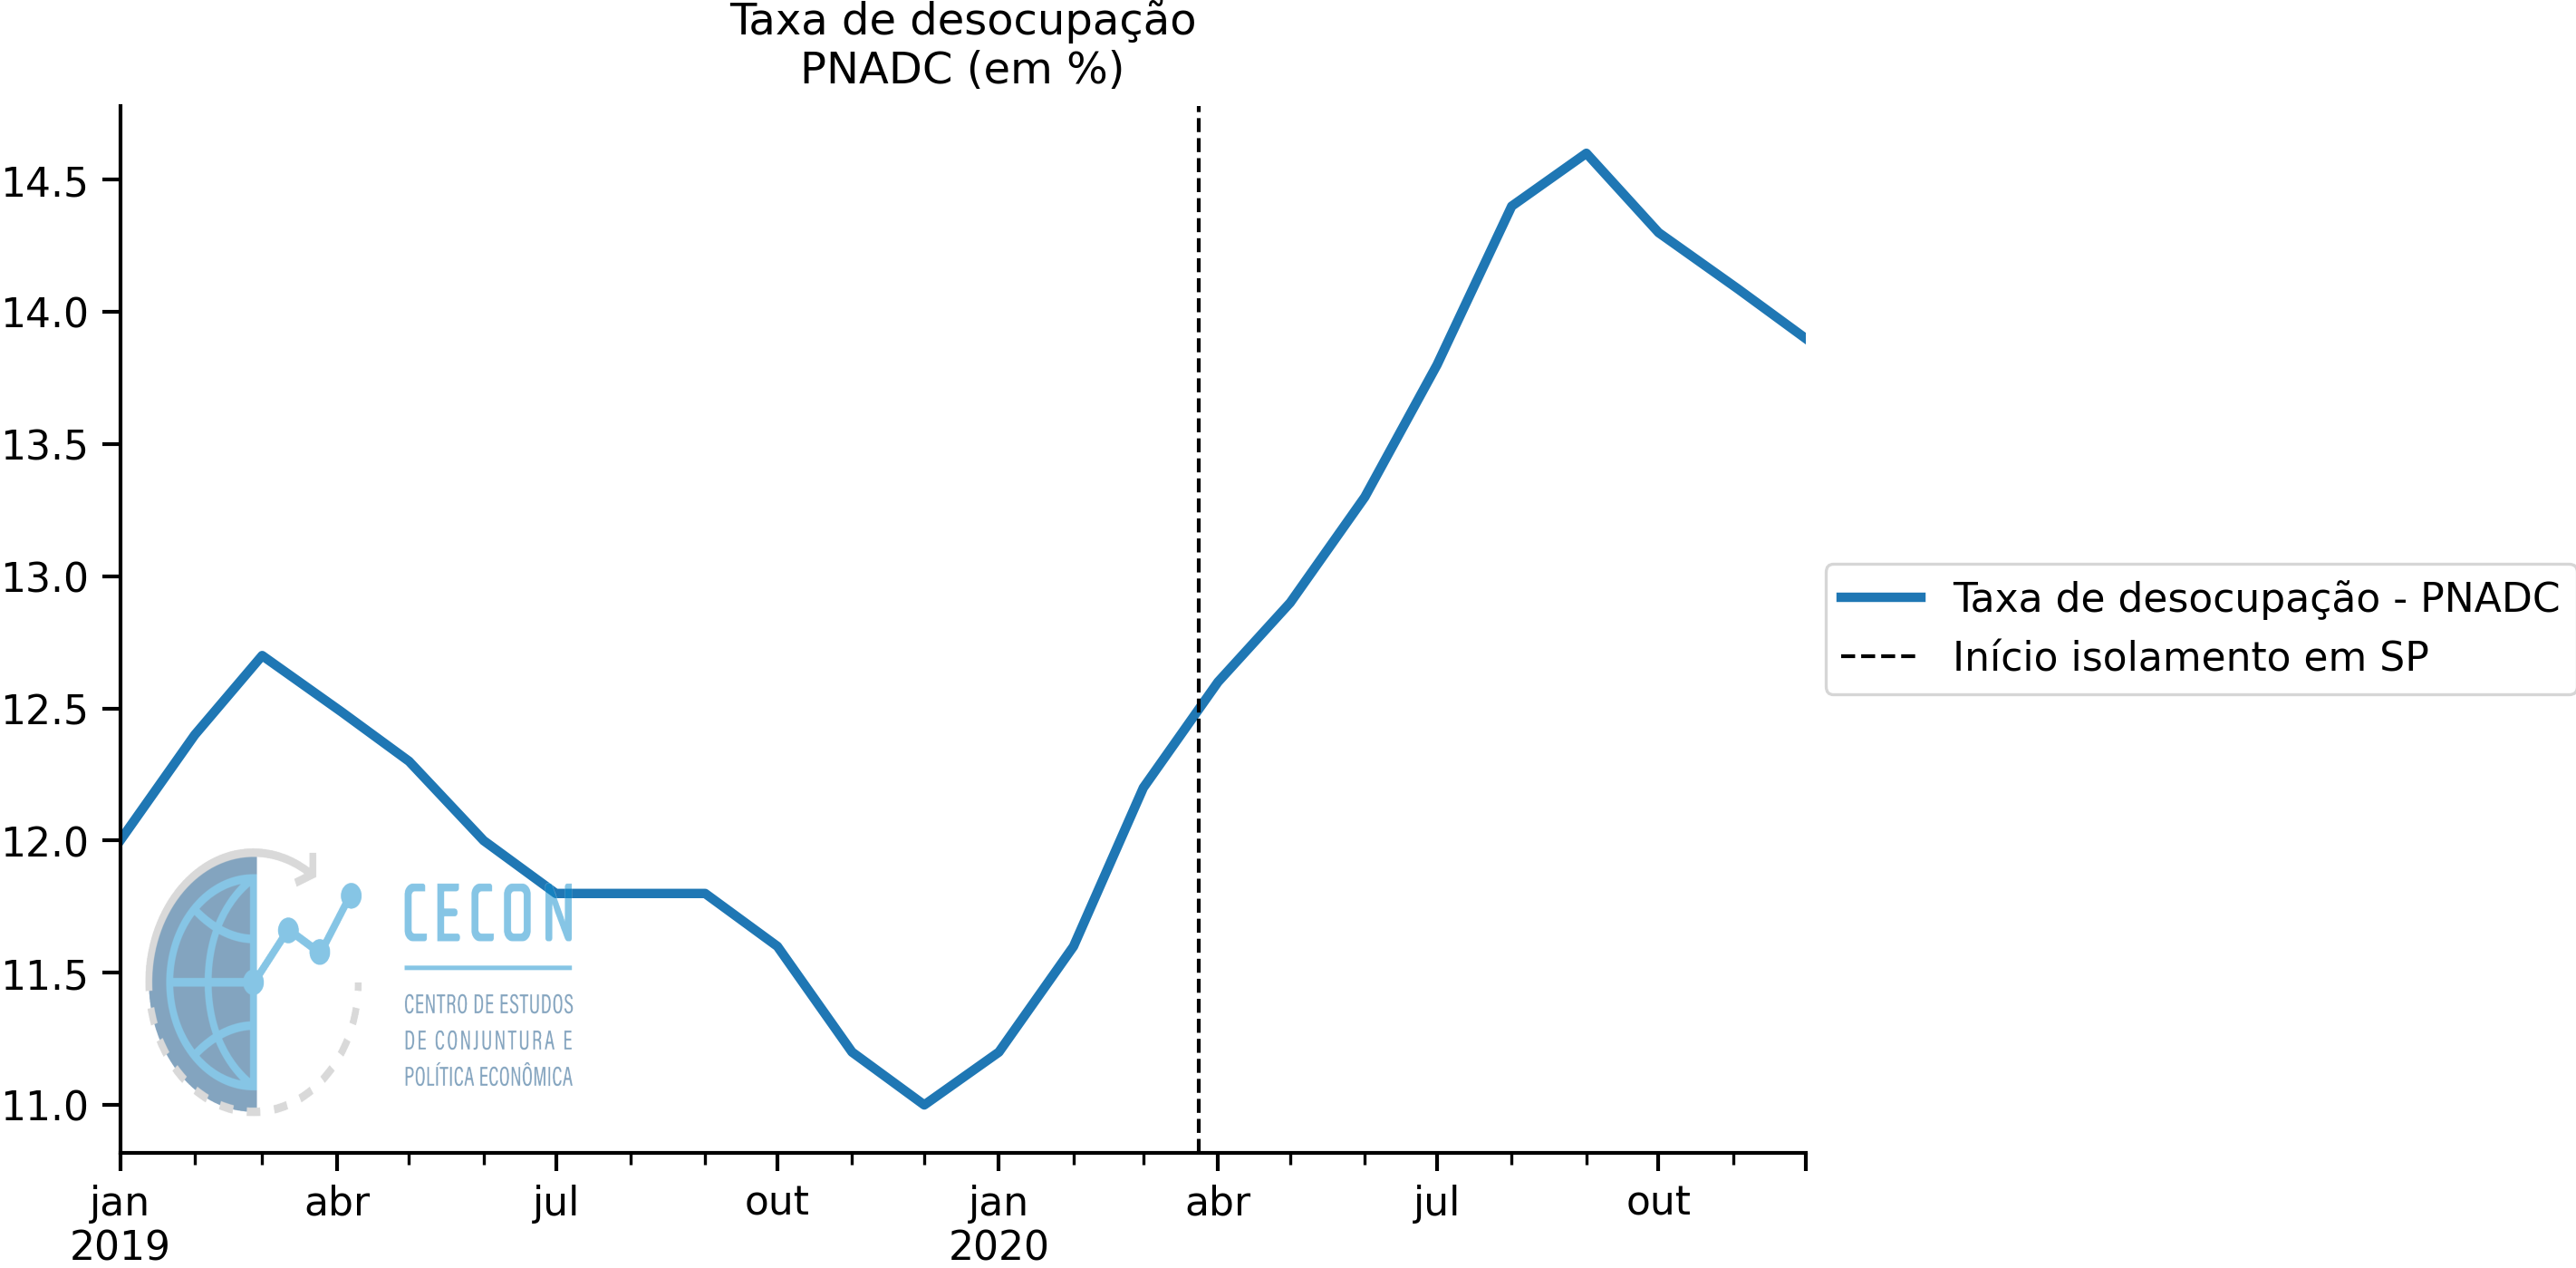
\includegraphics[width=.9\linewidth]{./figs/Emprego/TaxaDesocupacao.png}
\end{center}

\section*{PNAD-COVID}
\label{sec:orgfe6675c}
\subsection*{R trial}
\label{sec:org2497e9a}
\subsection*{Home office - Por sexo e cor}
\label{sec:org523c96c}




\begin{center}
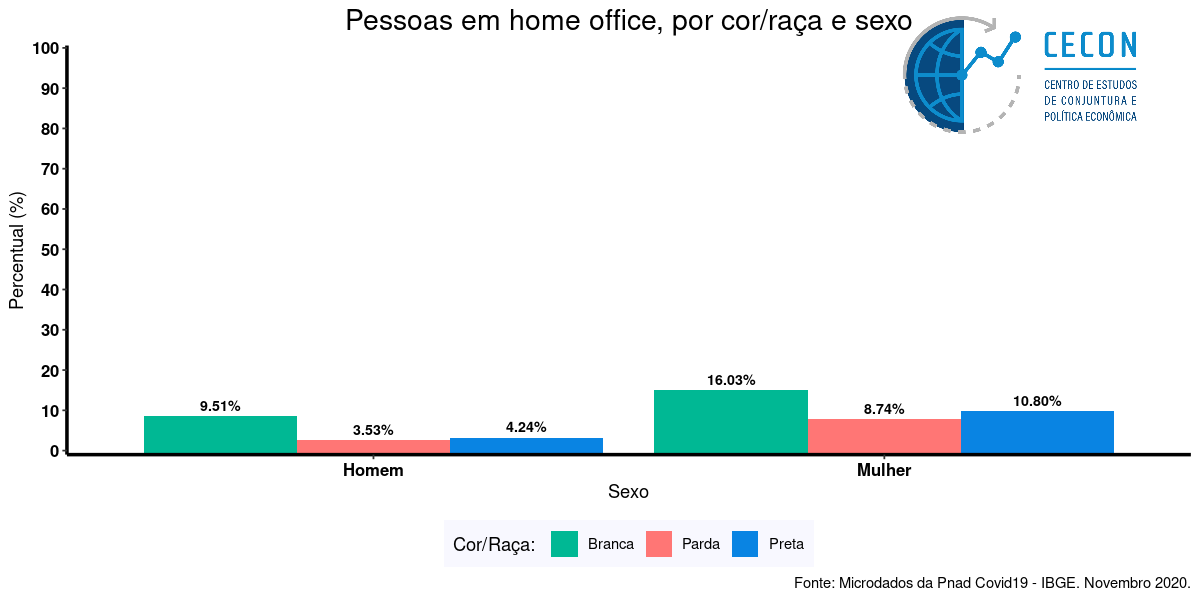
\includegraphics[width=.9\linewidth]{./figs/PNAD_COVID/home_sexo_cor.png}
\end{center}

\subsection*{Home office - Por Cor e Escolaridade}
\label{sec:orgf6bfd3a}
\begin{center}
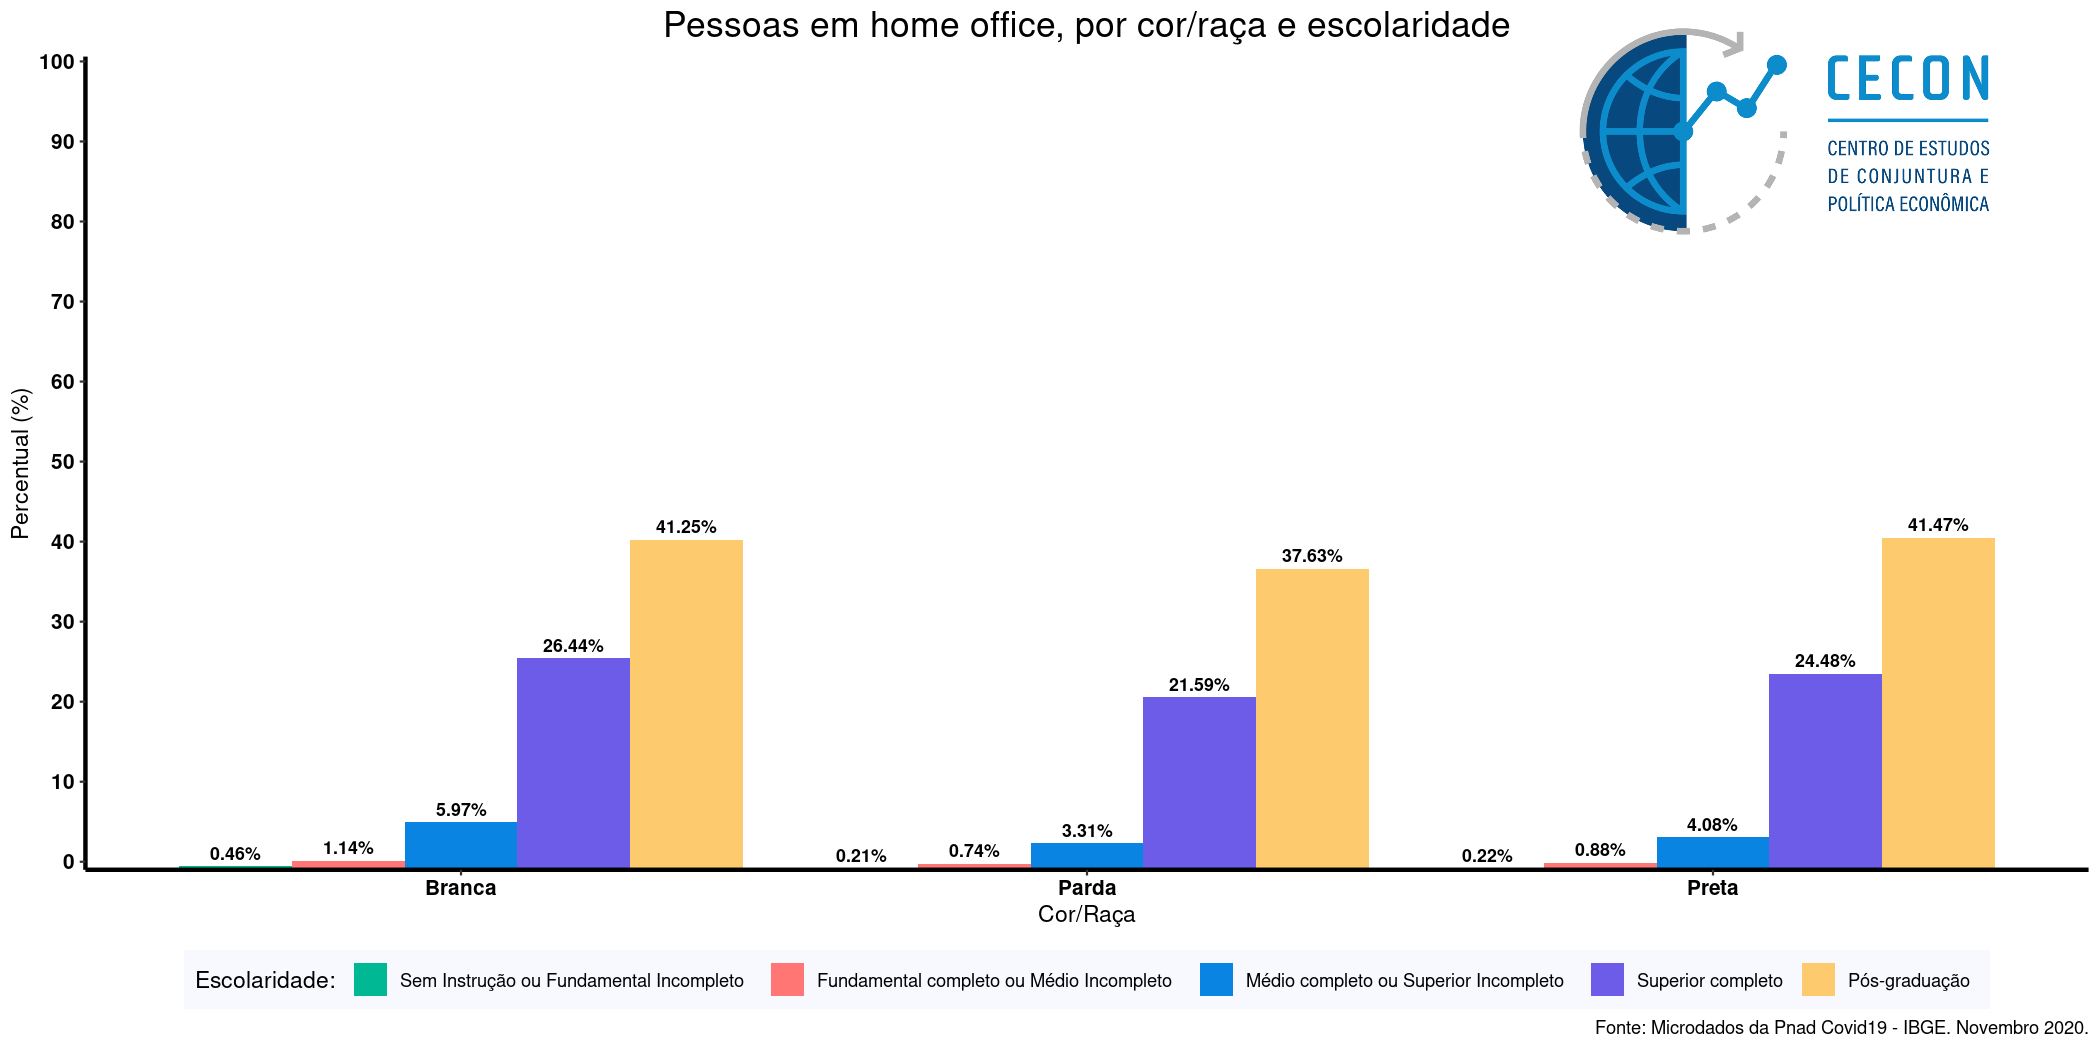
\includegraphics[width=.9\linewidth]{./figs/PNAD_COVID/home_edu_cor.png}
\end{center}
\subsection*{Home office - Por Cor e Idade}
\label{sec:orgc729242}
\begin{center}
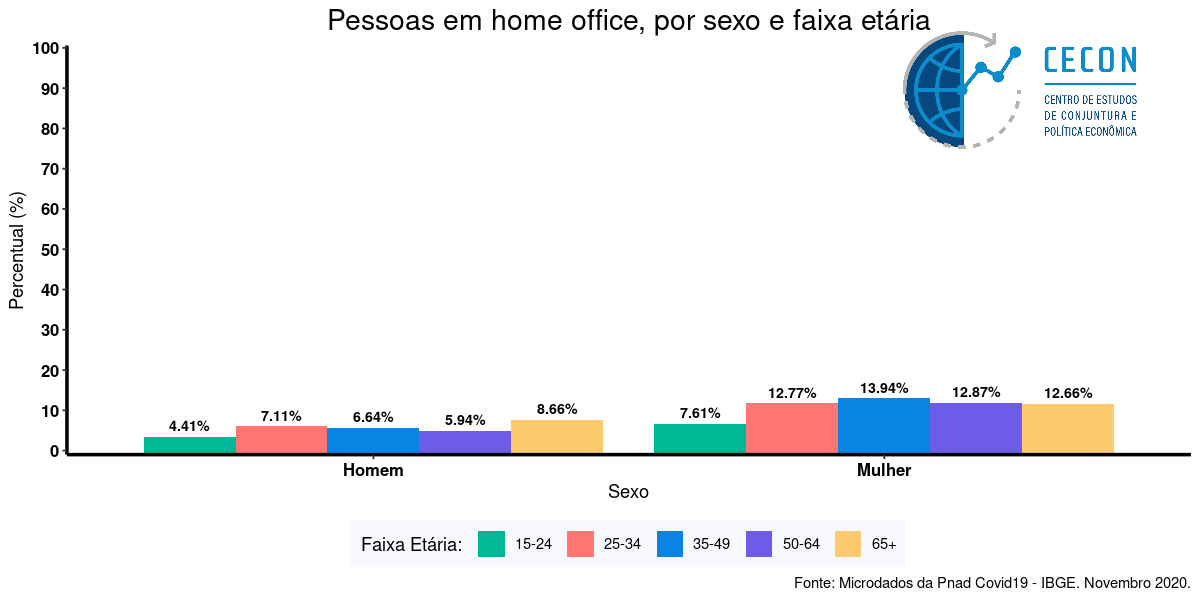
\includegraphics[width=.9\linewidth]{./figs/PNAD_COVID/home_sexo_idade.png}
\end{center}

\subsection*{Home office - Por Trabalho}
\label{sec:org83a37bb}
\begin{center}
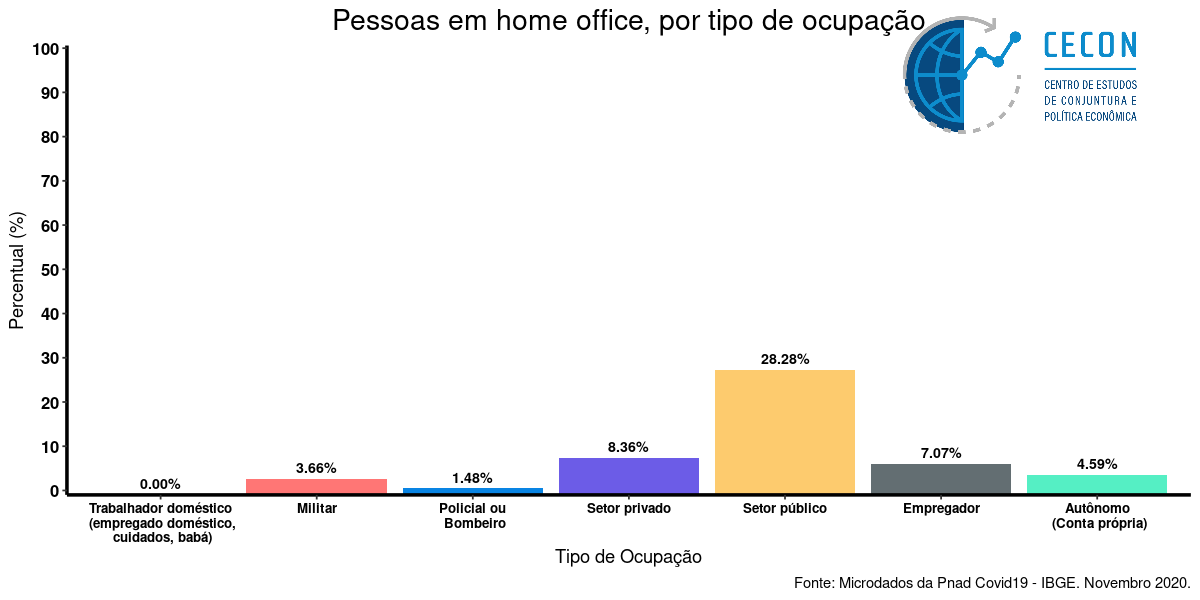
\includegraphics[width=.9\linewidth]{./figs/PNAD_COVID/home_emprego.png}
\end{center}

\subsection*{Home office - Por faixa salarial e cor}
\label{sec:org5ef8463}
\begin{center}
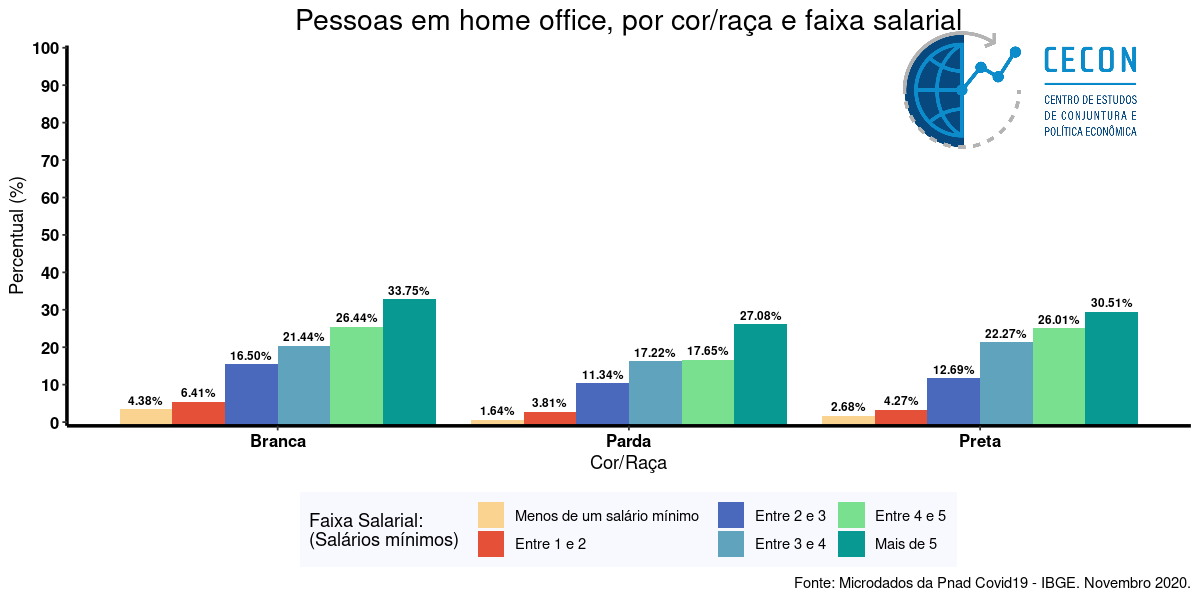
\includegraphics[width=.9\linewidth]{./figs/PNAD_COVID/home_renda.png}
\end{center}
\subsection*{Auxilio - Faixa Salarial}
\label{sec:org15d7f19}
\begin{center}
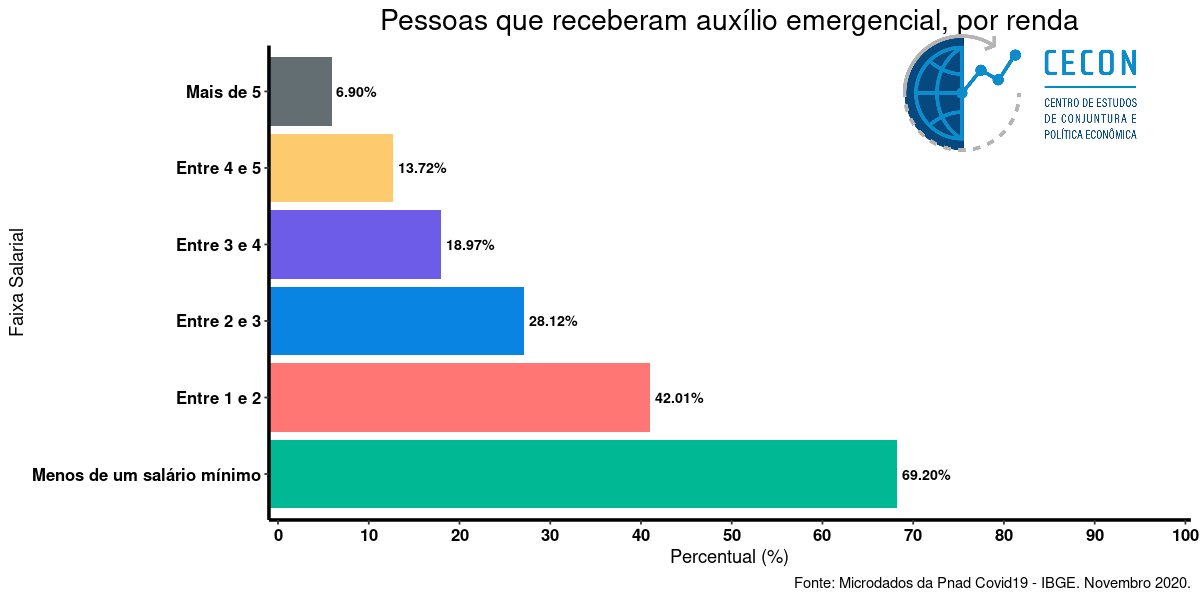
\includegraphics[width=.9\linewidth]{./figs/PNAD_COVID/auxilio_renda.png}
\end{center}
\subsection*{Auxilio - Por tipo do domicilio}
\label{sec:orgeefed92}
\begin{center}
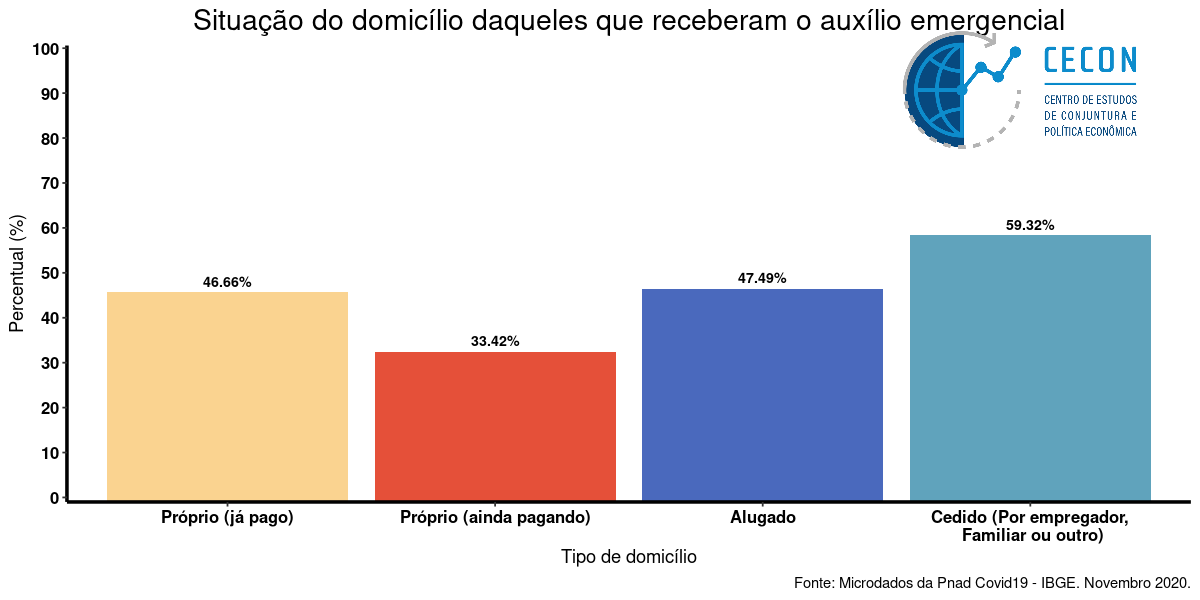
\includegraphics[width=.9\linewidth]{./figs/PNAD_COVID/auxilio_domicilio.png}
\end{center}
\subsection*{Auxilio - Sexo e Cor}
\label{sec:orgbfc76ec}
\begin{center}
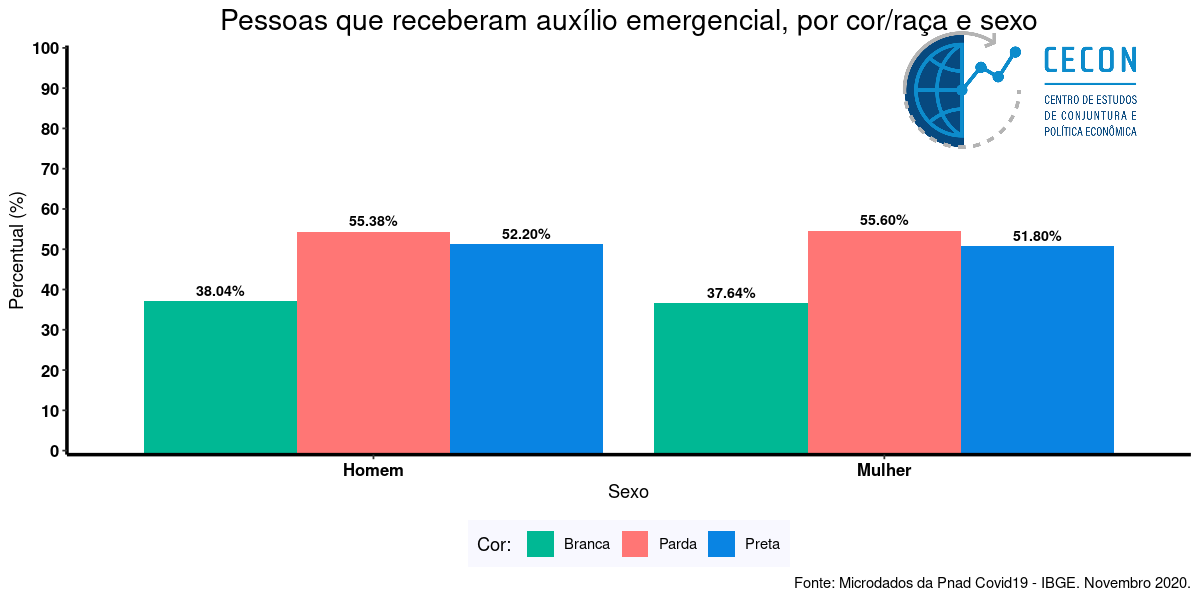
\includegraphics[width=.9\linewidth]{./figs/PNAD_COVID/auxilio_cor_sexo.png}
\end{center}


\section*{IMF Fiscal Monitor}
\label{sec:org736eb4a}
\subsection*{Medidas fiscais em \% do PIB}
\label{sec:org39cbf90}

\begin{center}
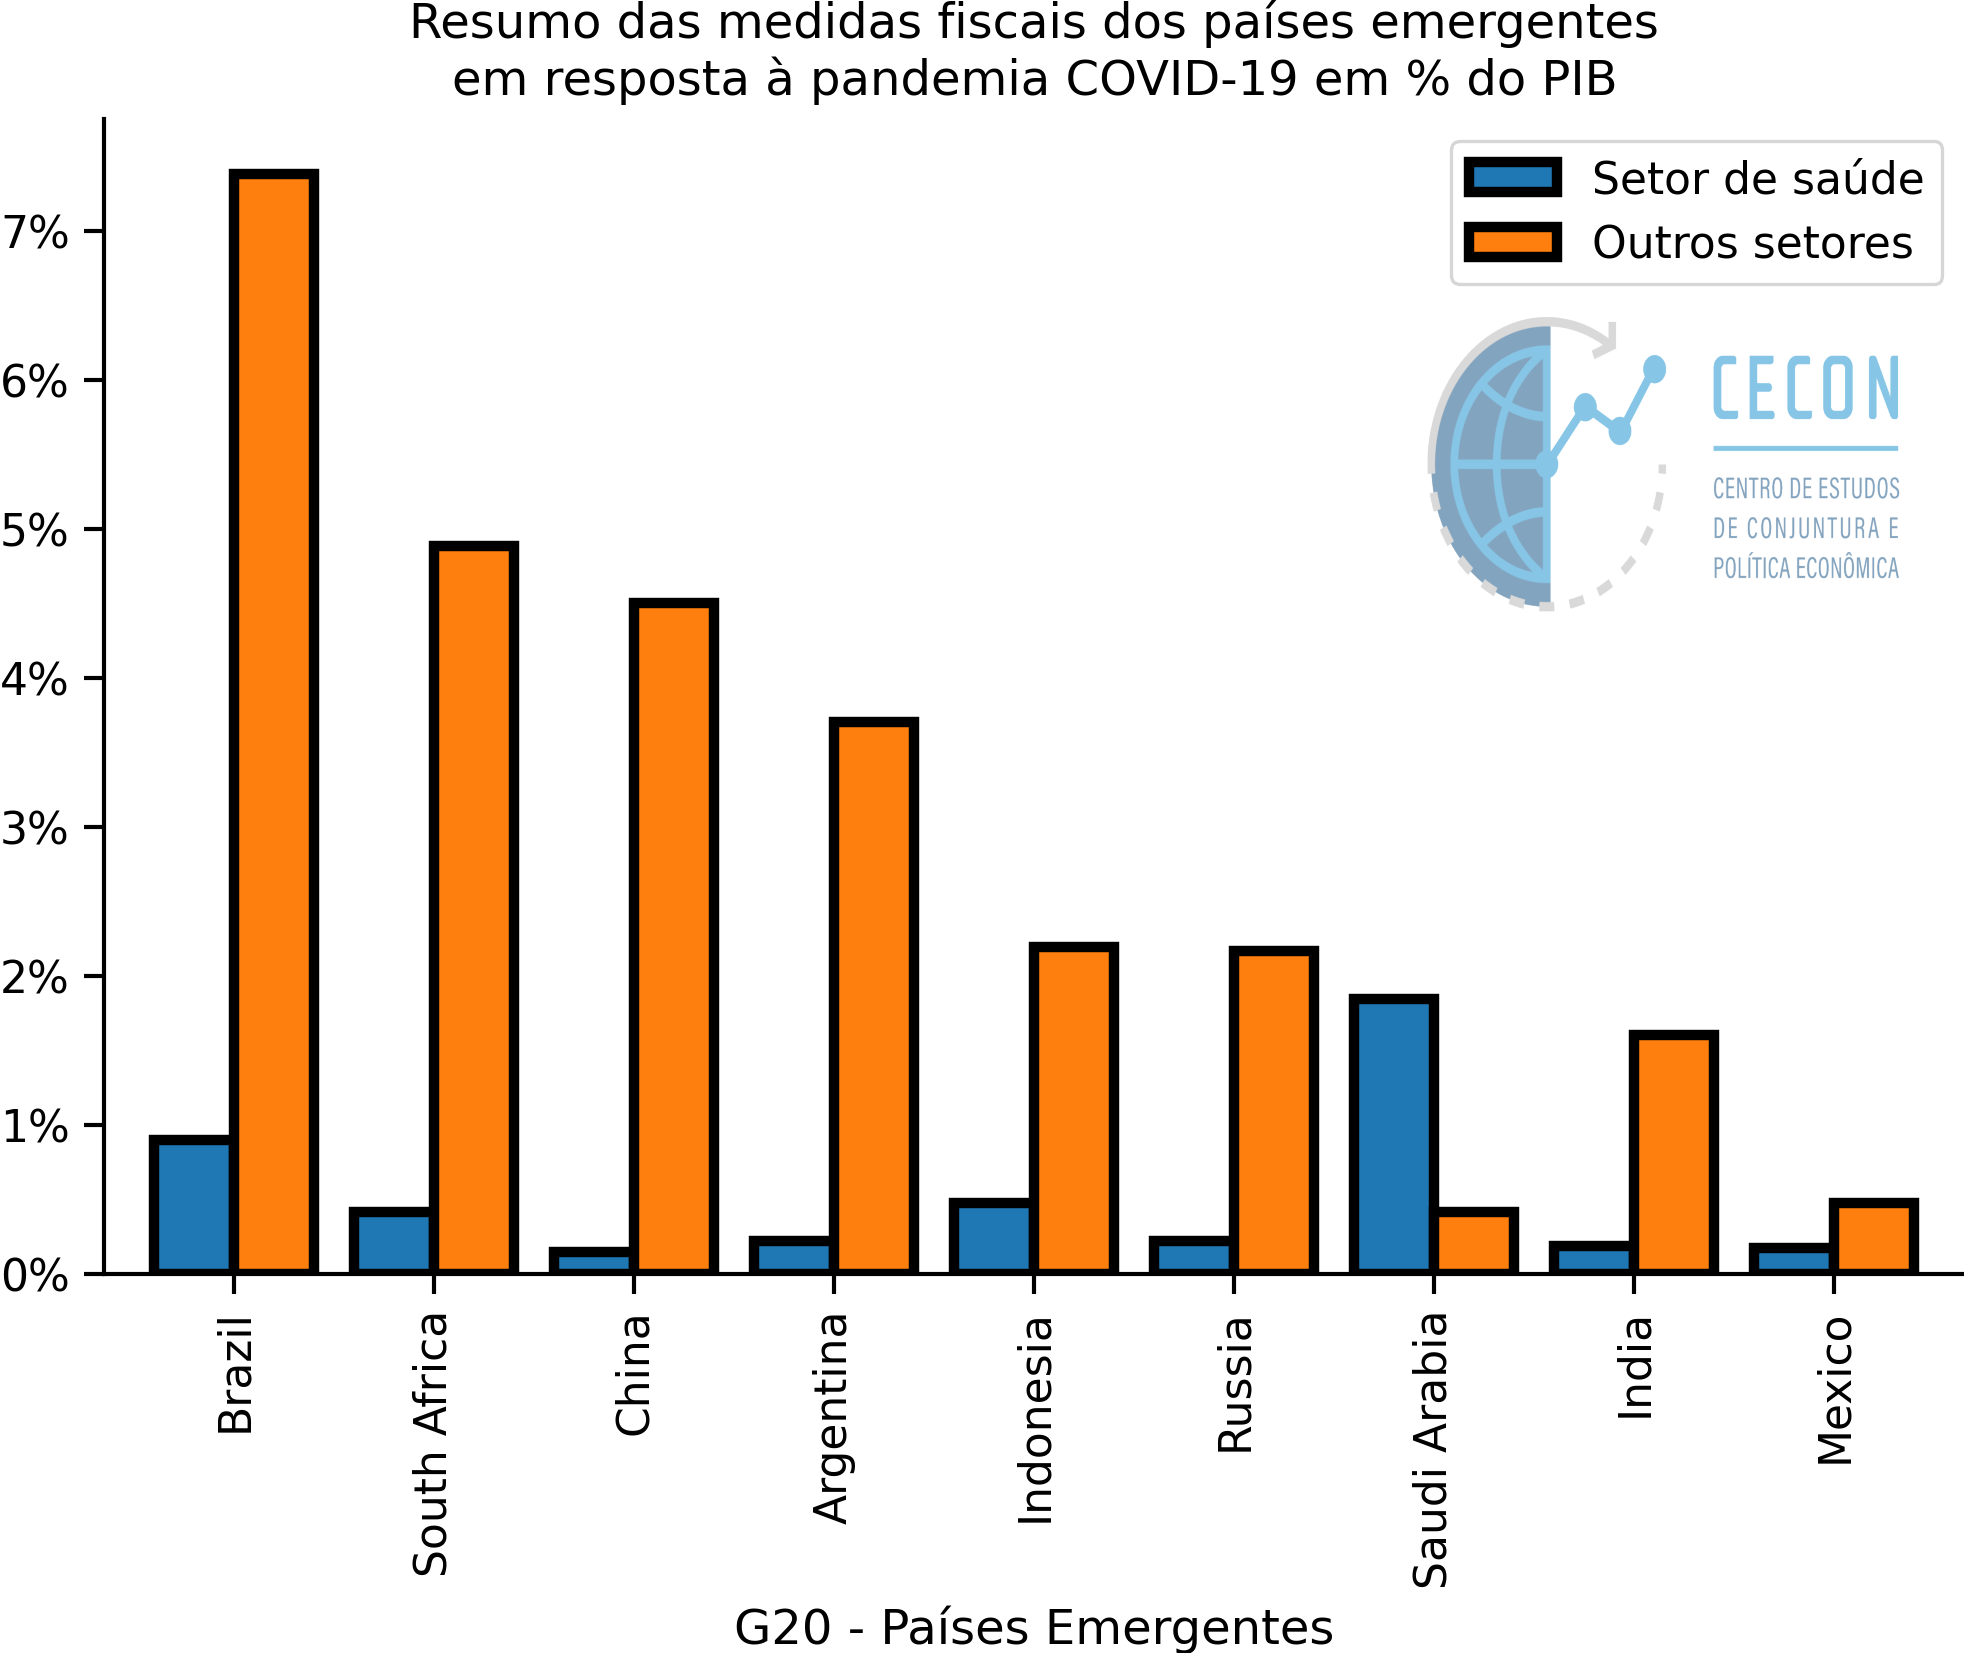
\includegraphics[width=.9\linewidth]{./figs/IMF/FiscalMonitor_Covid.png}
\end{center}

\subsection*{Medidas fiscais em \% do PIB: Setor de saúde/Outros setores}
\label{sec:orgdb7acc7}

\begin{center}
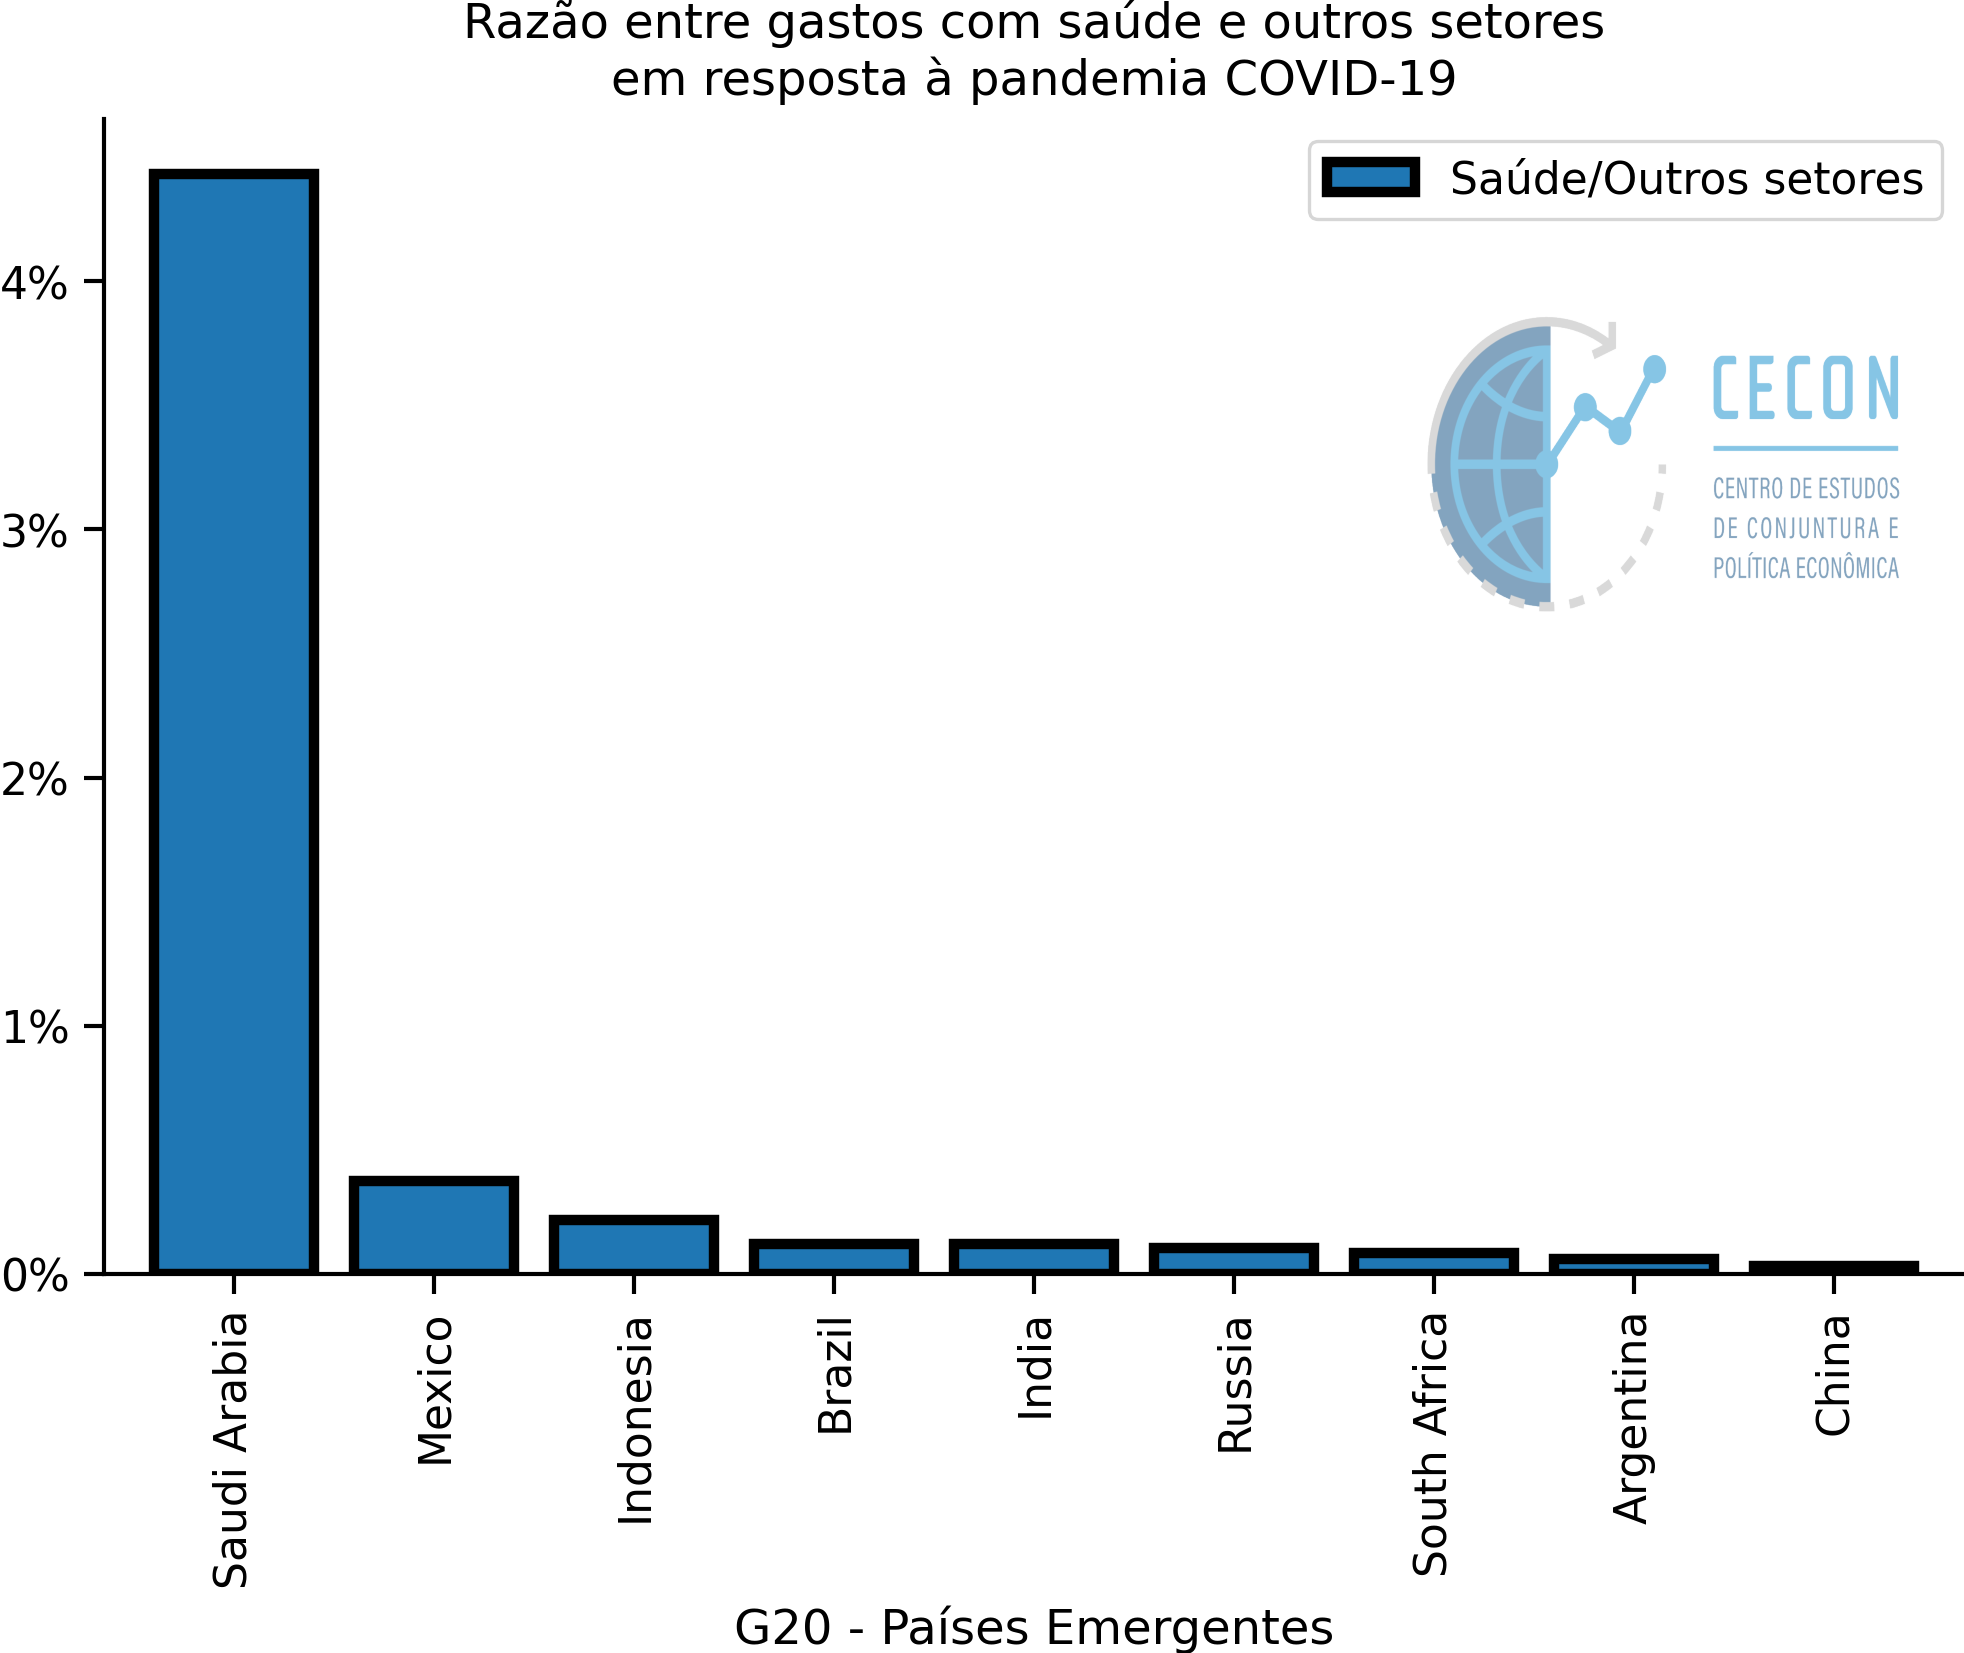
\includegraphics[width=.9\linewidth]{./figs/IMF/FiscalMonitor_Covid_ratio.png}
\end{center}

\subsection*{Medidas fiscais em \% do PIB: Setor de saúde/Total}
\label{sec:org34c07e1}

\begin{center}
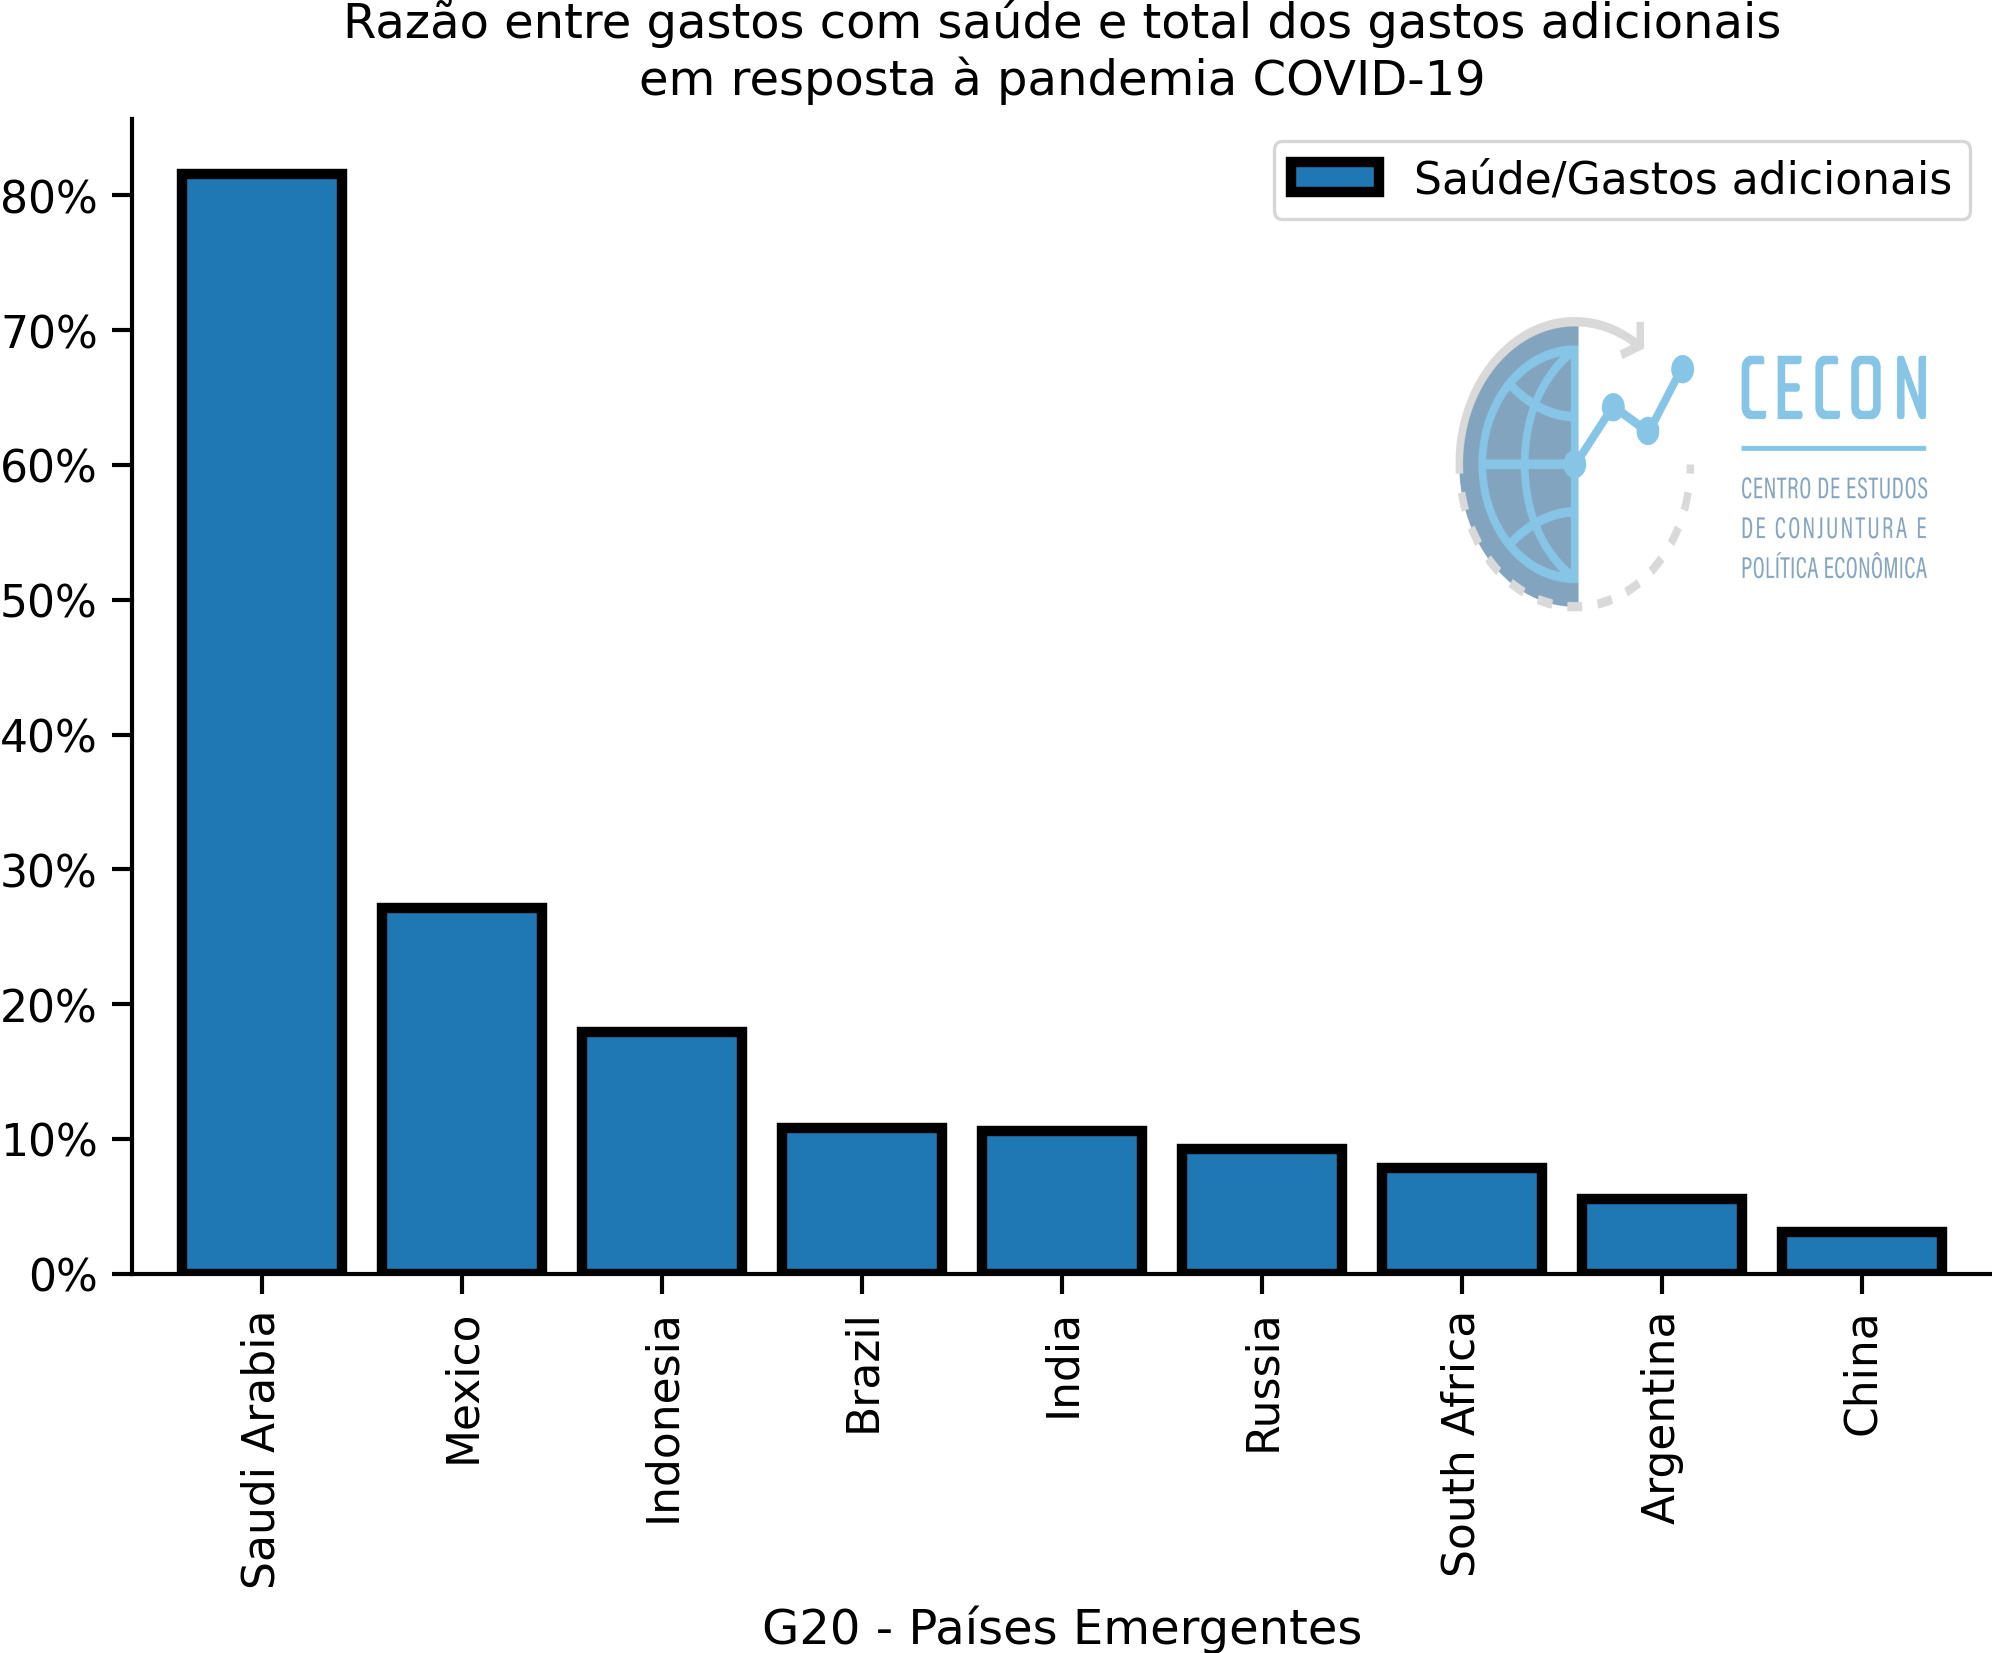
\includegraphics[width=.9\linewidth]{./figs/IMF/FiscalMonitor_Covid_total.png}
\end{center}

\section*{World Economic outlook}
\label{sec:org569686c}


\subsection*{GDP vs Lockdown}
\label{sec:org1845083}
\begin{table}[htbp]
\caption{\label{IMF_fig_1}GDP Forecast Errors in 2020:H1 and Lockdown Stringency}
\centering
\begin{tabular}{lll}
\hline
Country & GDP Forecast Error & Lockdown Stringency\\
\hline
AUS & -4,54 & 37,21\\
AUT & -9,11 & 37,13\\
BEL & -9,65 & 41,34\\
BRA & -8,71 & 44,01\\
CAN & -8,81 & 40,92\\
CHL & -5,71 & 41,76\\
CHN & -7,82 & 62,36\\
COL & -10,70 & 49,59\\
HRV & -9,36 & 40,25\\
CZE & -8,87 & 34,38\\
DNK & -6,03 & 39,22\\
EST & -6,54 & 31,58\\
FIN & -5,24 & 28,49\\
FRA & -13,44 & 48,72\\
DEU & -7,04 & 35,39\\
GRC & -10,79 & 39,91\\
HKG & -4,45 & 43,62\\
HUN & -8,91 & 38,69\\
IND & -15,70 & 51,69\\
IDN & -6,09 & 42,06\\
IRL & -3,48 & 45,59\\
ISR & -6,44 & 49,81\\
ITA & -11,99 & 51,65\\
JPN & -6,27 & 24,21\\
KOR & -3,02 & 39,64\\
LVA & -7,49 & 33,94\\
LTU & -3,51 & 40,30\\
MYS & -12,54 & 40,67\\
MEX & -11,10 & 41,61\\
NLD & -6,49 & 40,82\\
NOR & -6,10 & 32,55\\
PER & -20,54 & 55,43\\
PHL & -15,14 & 58,33\\
POL & -6,56 & 40,53\\
PRT & -10,87 & 43,79\\
ROU & -7,04 & 44,54\\
RUS & -4,29 & 48,61\\
SRB & -4,59 & 40,73\\
SGP & -7,63 & 43,65\\
SVK & -10,39 & 40,44\\
SVN & -11,35 & 34,24\\
ZAF & -9,66 & 47,21\\
ESP & -14,65 & 42,21\\
SWE & -4,28 & 21,08\\
CHE & -6,16 & 37,10\\
TWN & -1,37 & 13,73\\
THA & -9,13 & 39,43\\
TUR & -5,42 & 42,28\\
UKR & -8,08 & 47,94\\
GBR & -12,91 & 38,99\\
USA & -6,44 & 43,14\\
VNM & -4,35 & 47,91\\
\hline
\end{tabular}
\end{table}


\begin{center}
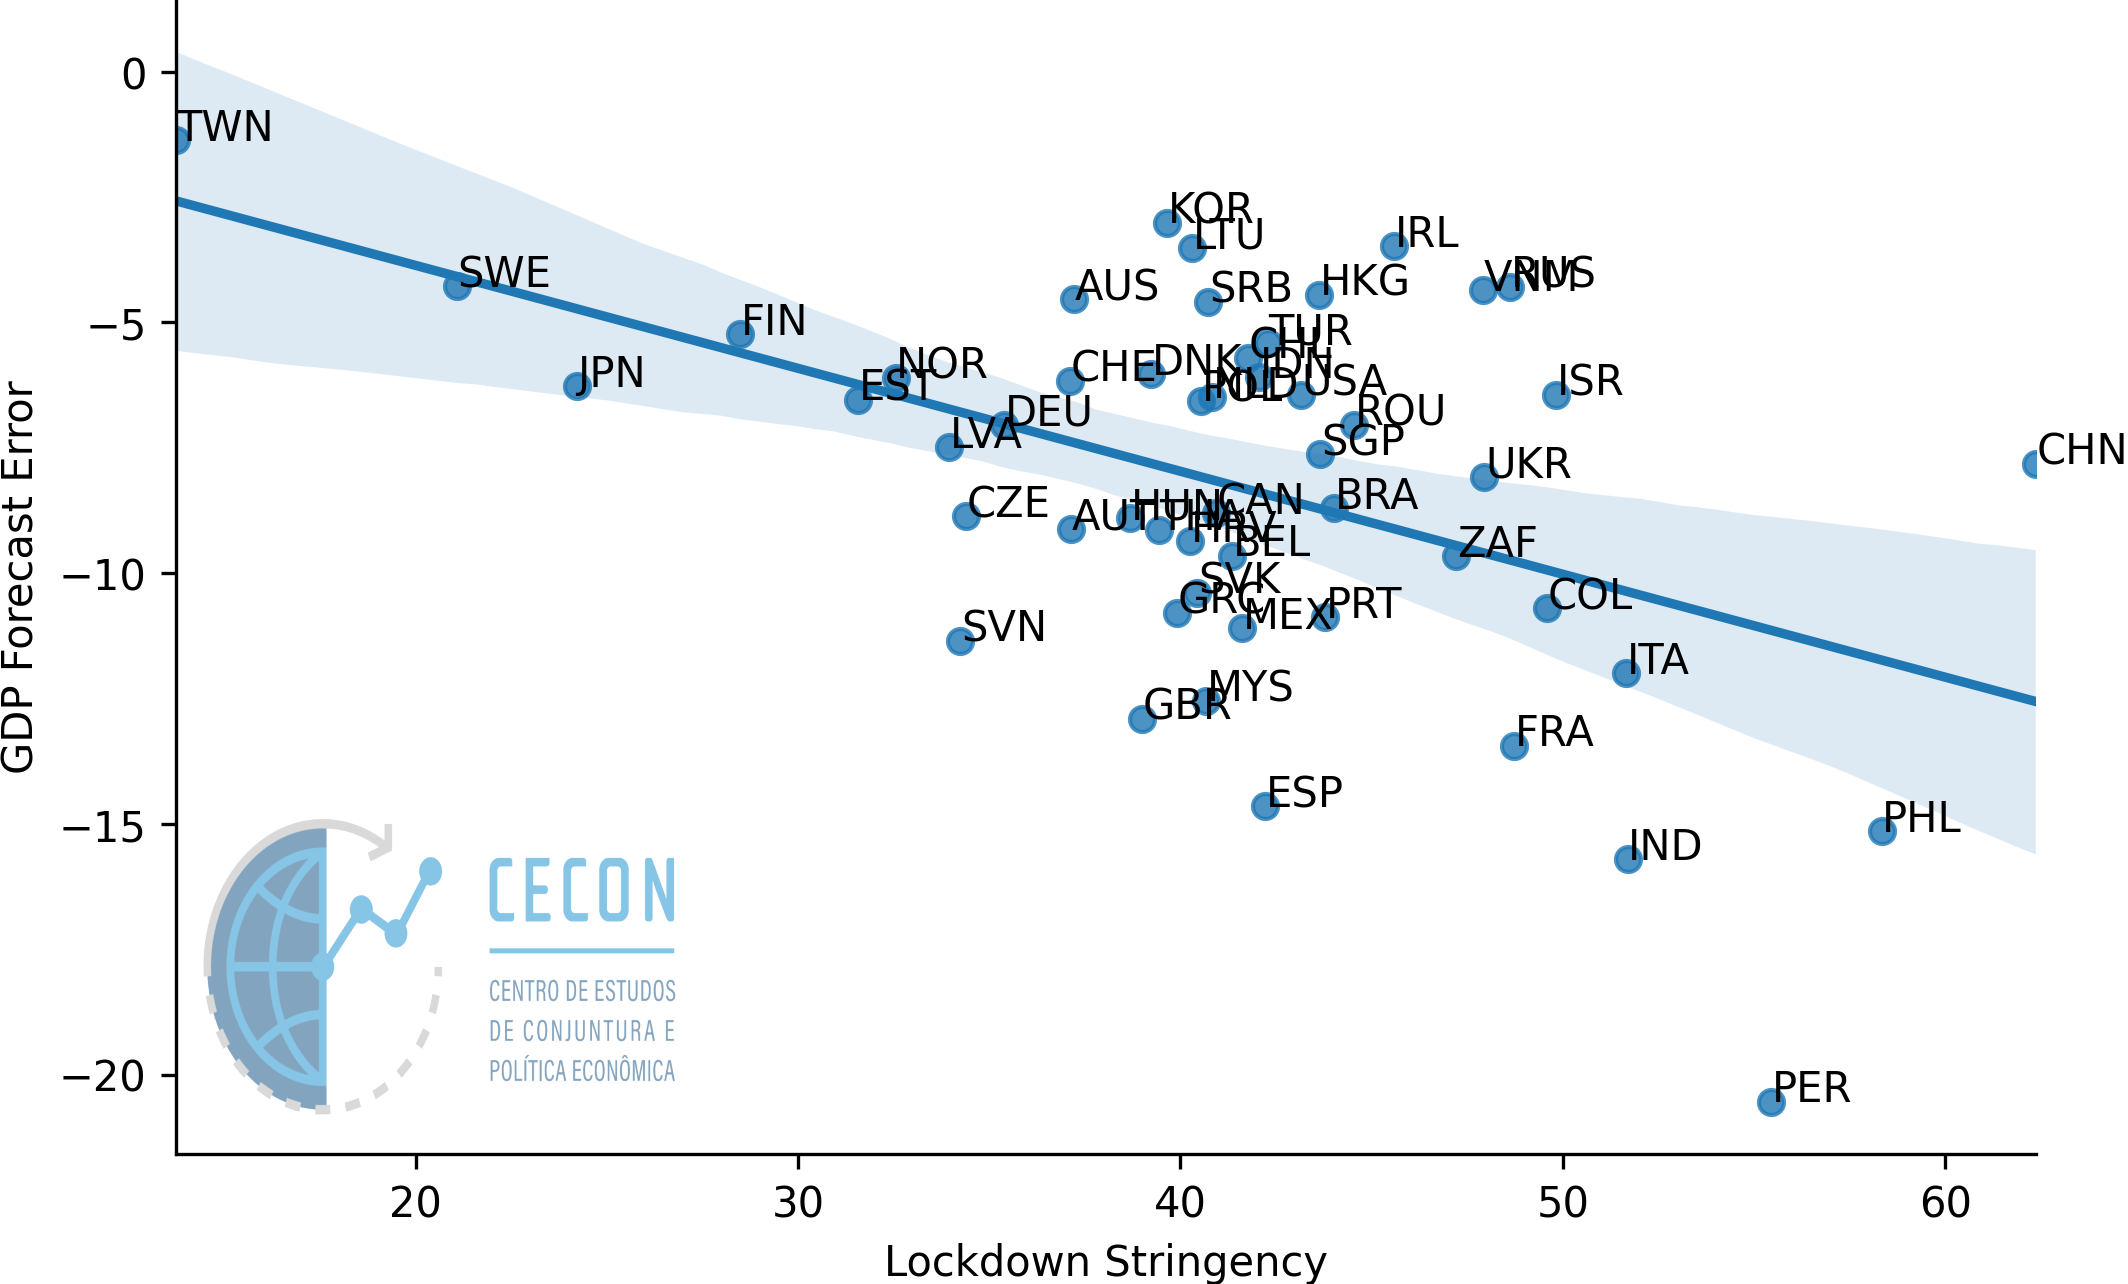
\includegraphics[width=.9\linewidth]{./figs/IMF/GDP_Lockdown.png}
\end{center}



\subsection*{Lockdown: Voluntary vs Stringency}
\label{sec:orgd801139}

\begin{table}[htbp]
\caption{\label{Vol_String}Impact of Lockdowns and Voluntary Social Distancing on Mobility during the First 90 Days of Each Country’s Epidemic}
\centering
\begin{tabular}{lll}
Country groups & Lockdown stringency & Voluntary social distancing\\
\hline
All & -7,85 & -6,53\\
AEs & -8,07 & -10,62\\
EMs & -8,78 & -6,26\\
LICs & -5,8 & -2,83\\
\hline
\end{tabular}
\end{table}

\begin{center}
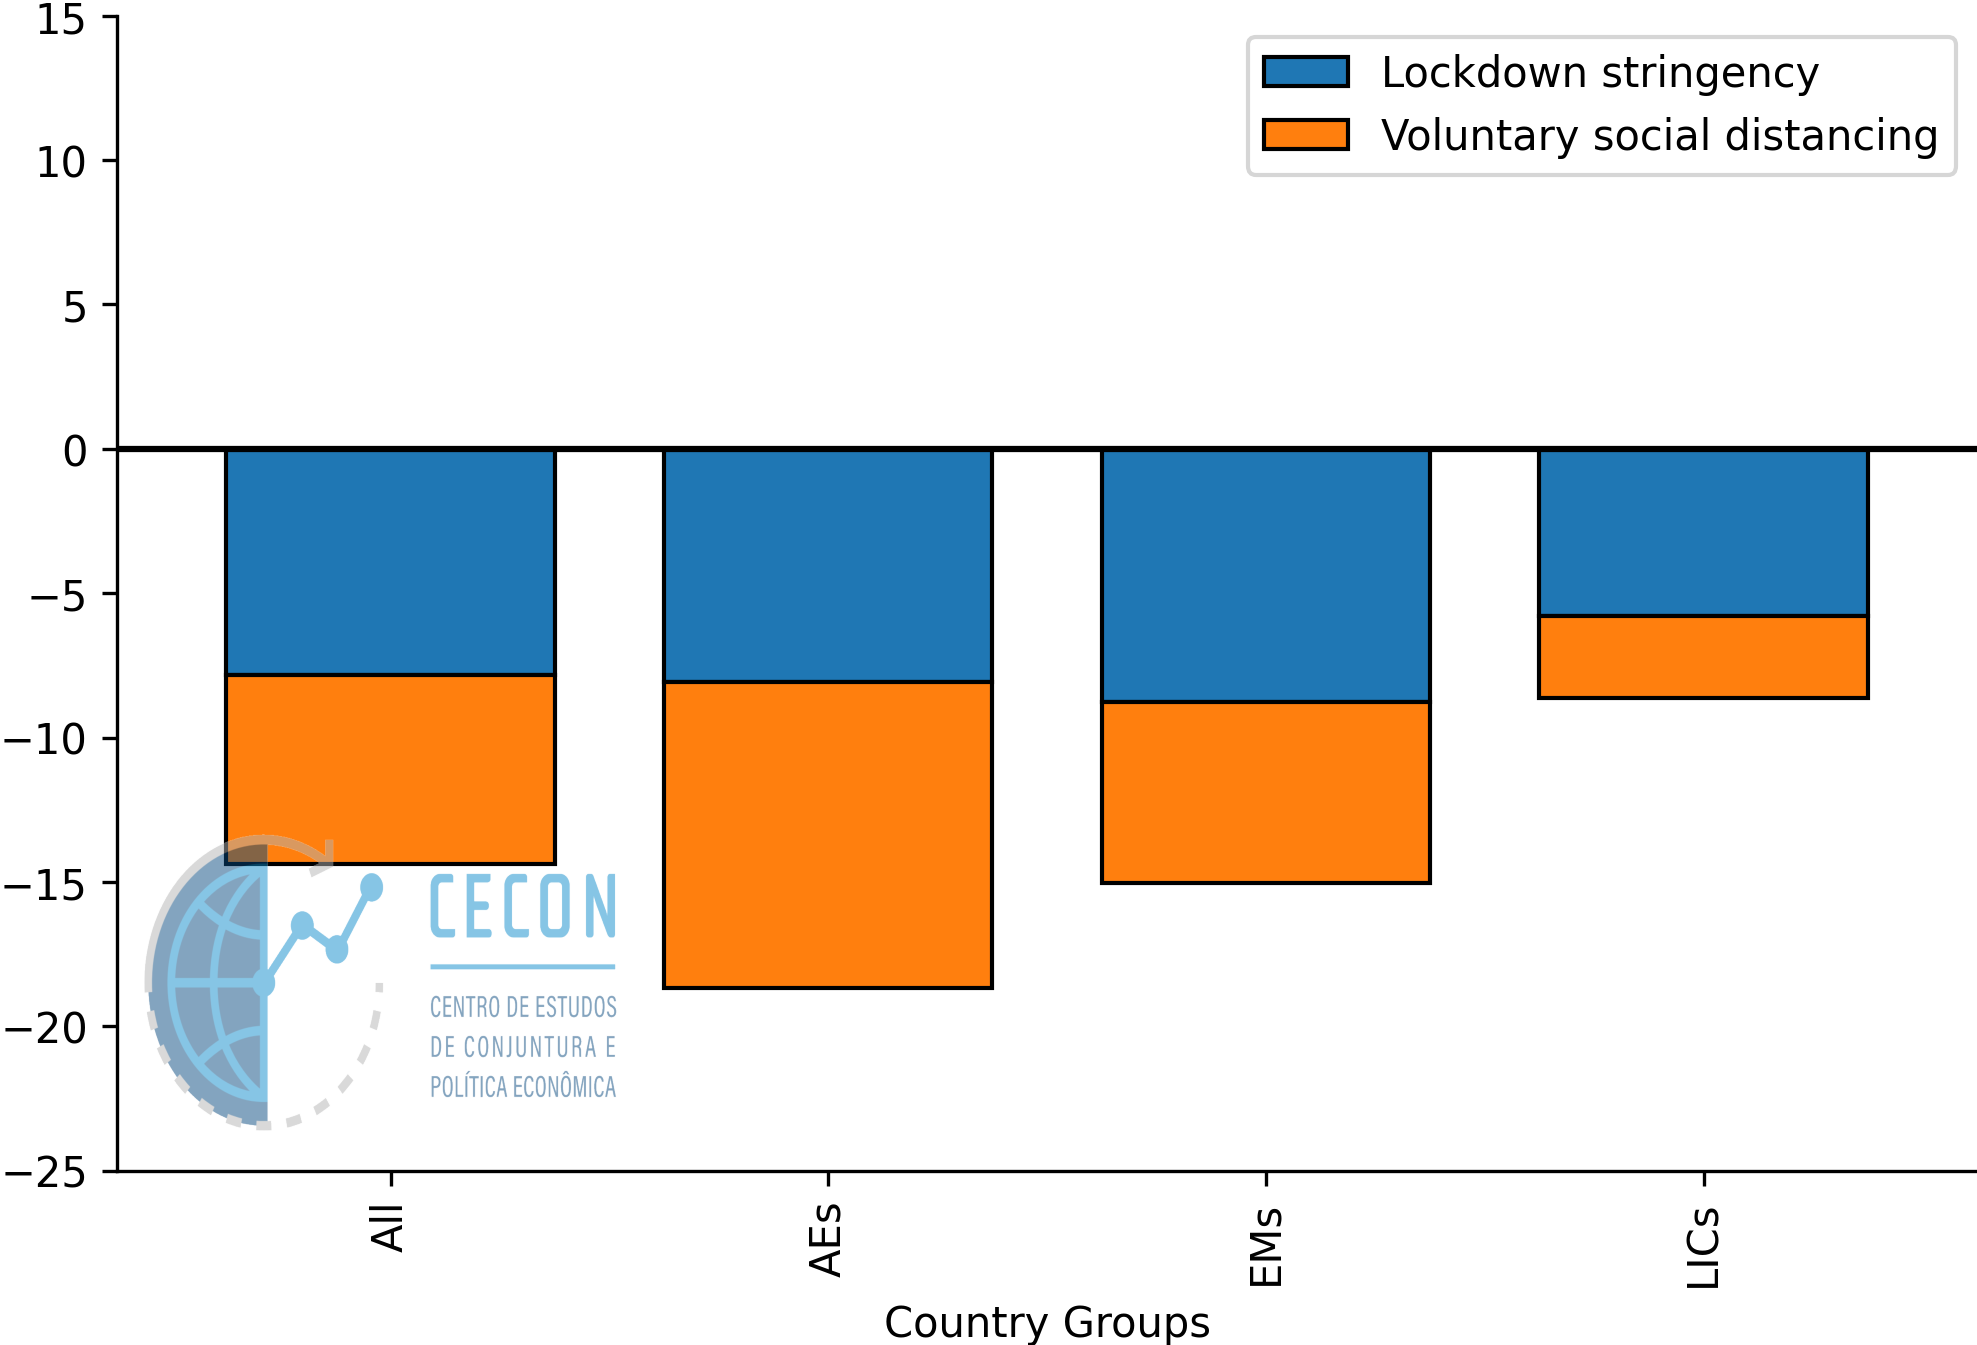
\includegraphics[width=.9\linewidth]{./figs/IMF/Vol_String.png}
\end{center}

\subsection*{Sequencing of lockdown measures}
\label{sec:orgdffb5a0}
\begin{table}[htbp]
\caption{\label{Lock_measure}Sequencing of lockdown measures}
\centering
\begin{tabular}{lrrr}
\hline
Lockdown measures & Middle & Low & High\\
\hline
Stay-at-home orders & 18 & 10 & 27\\
Public transport closures & 16 & 7,5 & 25\\
Internal movement restrictions & 16 & 7 & 27\\
Workplace closures & 13 & 6 & 22\\
Gathering restrictions & 10 & 2 & 20\\
Public event cancellations & 6 & 1 & 14,5\\
School closures & 4,5 & 1 & 13,5\\
International travel controls & 1 & 0 & 9\\
\hline
\end{tabular}
\end{table}

\begin{center}
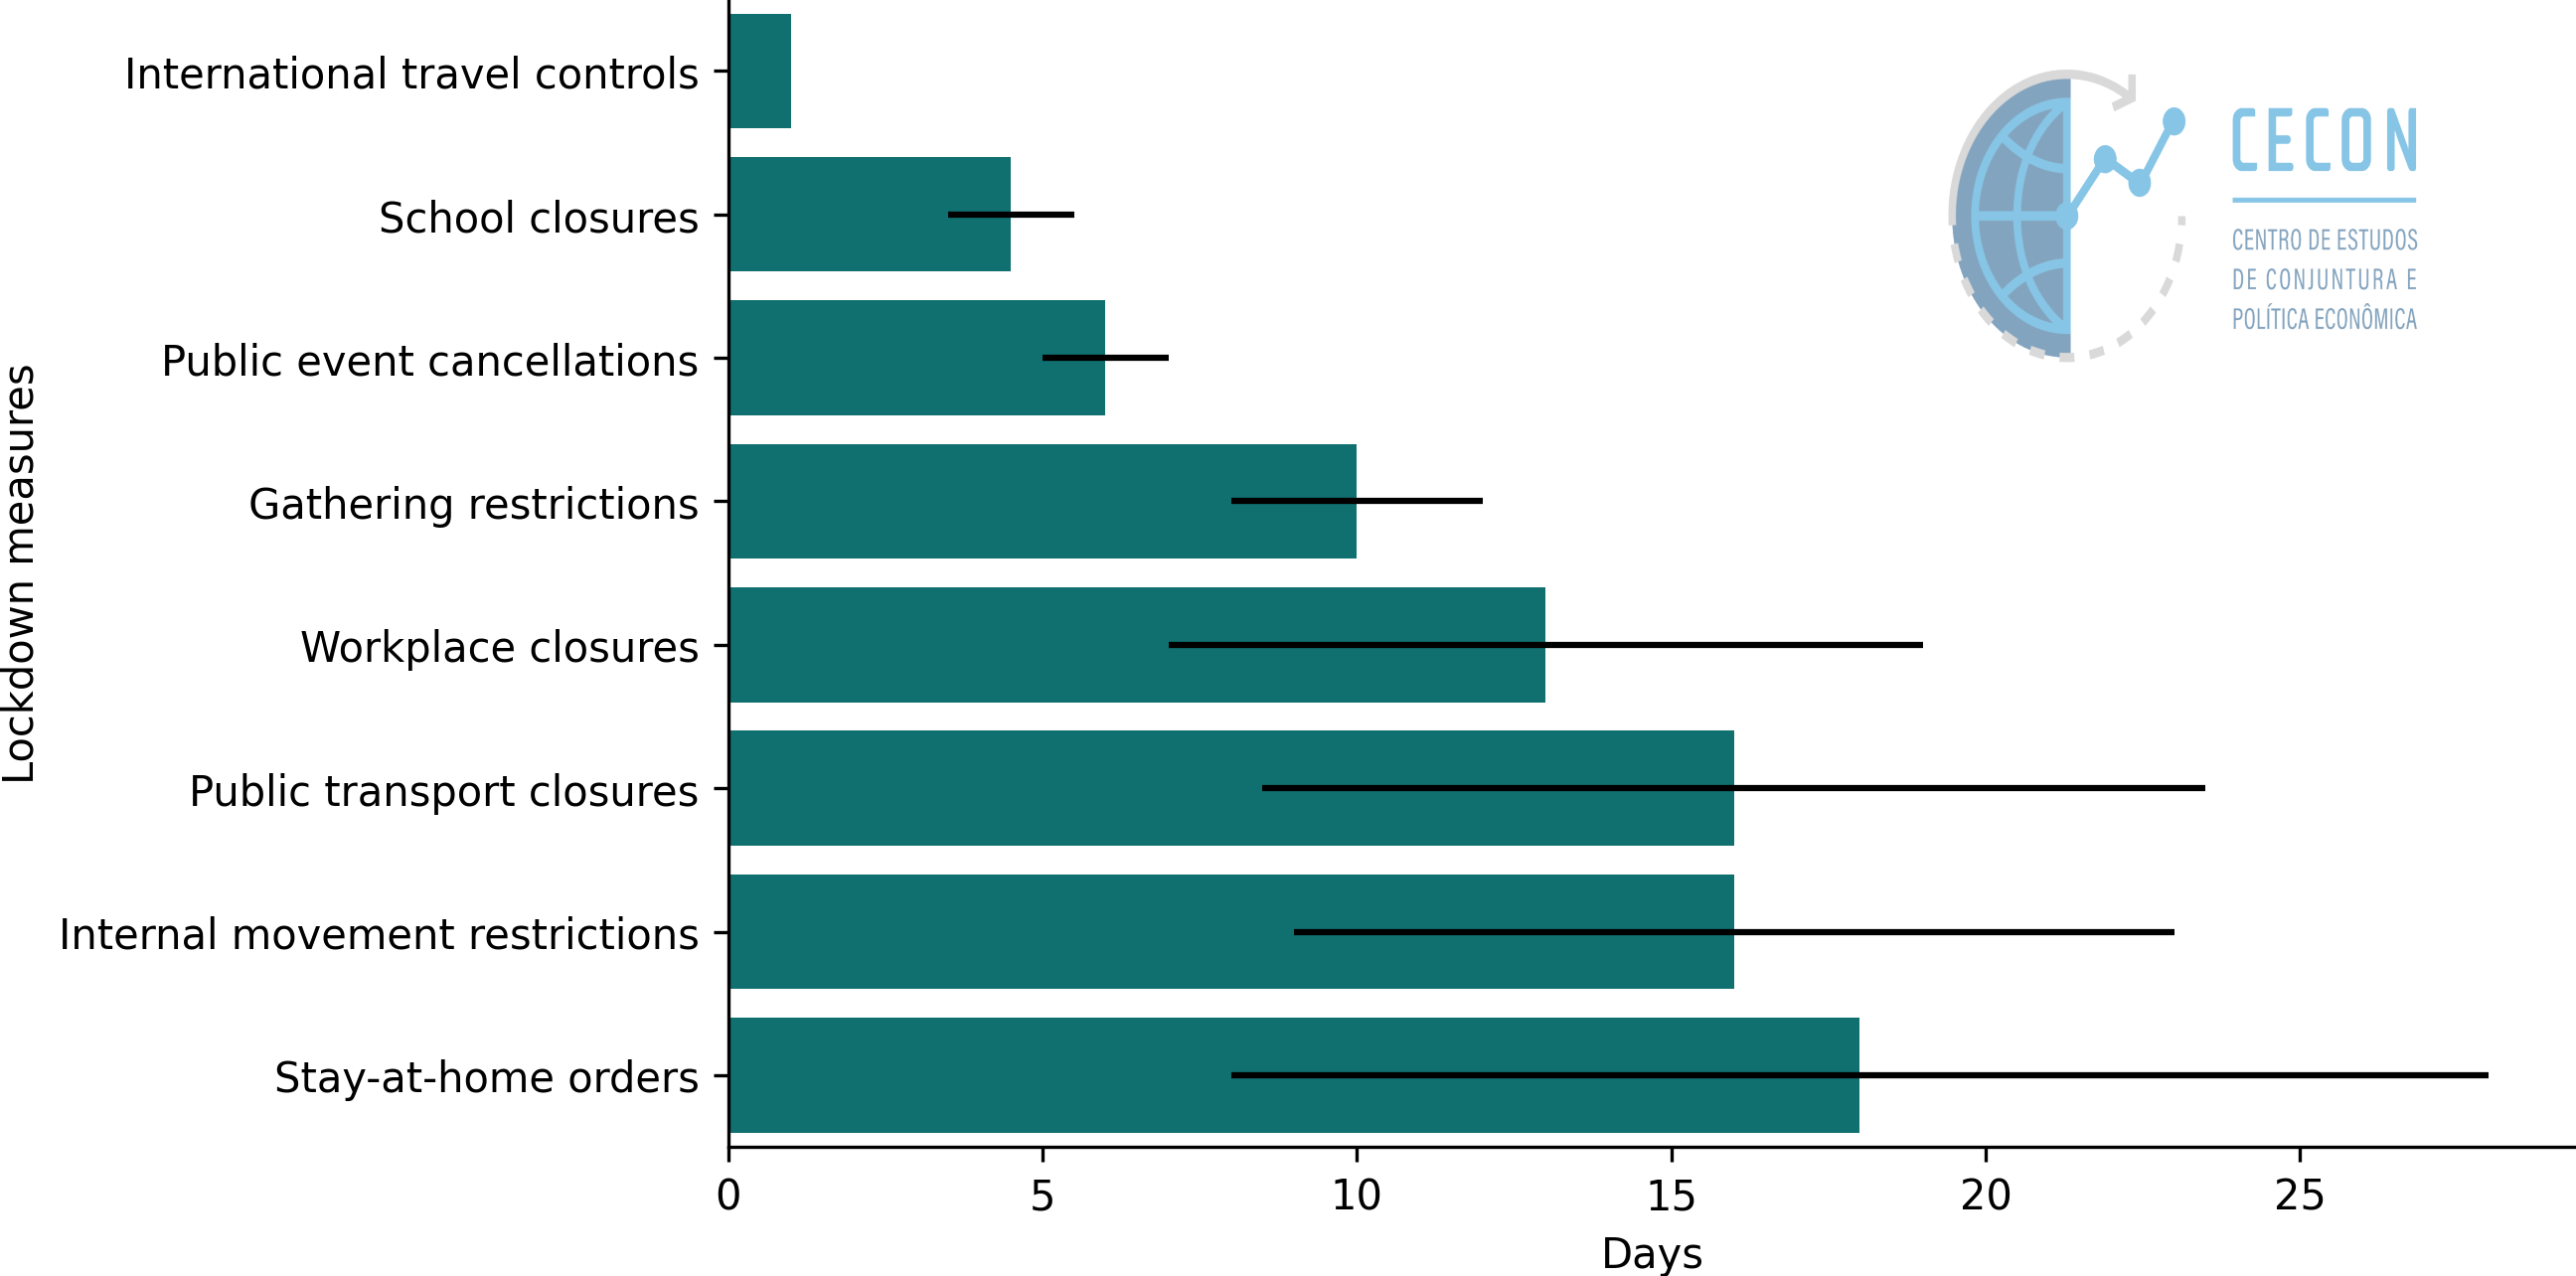
\includegraphics[width=.9\linewidth]{./figs/IMF/Lock_measures.png}
\end{center}
\end{document}
